%% IFBTcc Latex Template Version
%% 	based on a fork of : RiSE Latex Template
%%
%% IFBthesis latex template for thesis and dissertations
%% https://github.com/IFBmodels/tcc
%%
%% (c) 2017 Rafael de Campos Passos (rcpassos@ieee.org)
%%
%% This document was initially based on RiSE Latex template, from Yguaratã
%% Cerqueira Cavalcanti
%%
%% GENERAL INSTRUCTIONS
%%
%% We strongly recommend you to compile your documents using pdflatex command.
%% It is also recommend use the texlipse plugin for Eclipse to edit your documents.
%%
%% Options for \documentclass command:
%%         * Idiom
%%           pt   - Portguese (default)
%%           en   - English
%%
%%         * Text type
%%           bsc  - B.Sc. Thesis
%%           msc  - M.Sc. Thesis (default)
%%           qual - PHD qualification (not tested yet)
%%           prop - PHD proposal (not tested yet)
%%           phd  - PHD thesis
%%
%%         * Media
%%           scr  - to eletronic version (PDF) / see the users guide
%%
%%         * Pagination
%%           oneside - unique face press
%%           twoside - two faces press
%%
%%		   * Line spacing
%%           singlespacing  - the same as using \linespread{1}
%%           onehalfspacing - the same as using \linespread{1.3}
%%           doublespacing  - the same as using \linespread{1.6}
%%
%% Reference commands. Use the following commands to make references in your
%% text:
%%          \figref  -- for Figure reference
%%          \tabref  -- for Table reference
%%          \eqnref  -- for equation reference
%%          \chapref -- for chapter reference
%%          \secref  -- for section reference
%%          \appref  -- for appendix reference
%%          \axiref  -- for axiom reference
%%          \conjref -- for conjecture reference
%%          \defref  -- for definition reference
%%          \lemref  -- for lemma reference
%%          \theoref -- for theorem reference
%%          \corref  -- for corollary reference
%%          \propref -- for proprosition reference
%%          \pgref   -- for page reference
%%
%%          Example: See \chapref{chap:introduction}. It will produce
%%                   'See Chapter 1', in case of English language.
%%
%% Citation commands:
%%          \citet (from natbib) -- To cite a reference as part of the narrative
%%          \citep (from natbib) -- To cite a reference between parenthesis
%%          citationblock environment -- To produce direct citation blocks according to the ABNT
\documentclass[pt,twoside,onehalfspacing,bsc]{ifbclass/ifbclass}
  \usepackage{colortbl}
  \usepackage{color}
  \usepackage[table]{xcolor}
  \usepackage{microtype}
  \usepackage{bibentry}
  \usepackage{subfigure}
  \usepackage{multirow}
  \usepackage{rotating}
  \usepackage{booktabs}
  \usepackage{pdfpages}
  \usepackage{caption}
  \usepackage{lipsum}
  \usepackage{sectsty}
  \usepackage{tikz}
  \usepackage{amsmath}
  \usepackage{url}
  \usepackage{minted}
  \usepackage{newfloat}
  \usepackage{float}
  \usepackage{xcolor}
  \usepackage{longtable}
  \usepackage{array}
  \usepackage{booktabs}
  \usepackage{multirow}
  \usepackage{caption}
  \usepackage{adjustbox}
  \usepackage{longtable}
  
  %% Set the language used in your code in the block above
  
  \captionsetup[table]{position=top,justification=centering,width=.85\textwidth,labelfont=bf,font=footnotesize}
  \captionsetup[lstlisting]{position=top,justification=centering,width=.85\textwidth,labelfont=bf,font=footnotesize}
  \captionsetup[figure]{position=bottom,justification=centering,width=.85\textwidth,labelfont=bf,font=footnotesize}

  % \renewcommand{\listingname}{Código}
  \renewcommand{\listingscaption}{Código}

  \setminted{
    fontsize=\scriptsize,
    linenos,
    breaklines,
    autogobble
  }

  %% Chapter and (Sub)Section fonts must be same size as text (12)
  \sectionfont{\fontsize{12}{15}\selectfont}
  \subsectionfont{\fontsize{12}{15}\selectfont}
  \subsubsectionfont{\fontsize{12}{15}\selectfont}
  
  %% Change the following pdf author attribute name to your name.
  \usepackage[linkcolor=black,
              citecolor=black,
              urlcolor=black,
              colorlinks,
              pdfpagelabels,
              pdftitle={IFB tcc Template (ABNT)},
              pdfauthor={ifb ctag team},
              breaklinks=true]{hyperref}
  
  \address{BRASÍLIA}
  
  \universitypt{Instituto Federal de Educação, Ciência e Tecnologia de Brasília, \textit{campus} Taguatinga,}
  \universityen{Federal Institute of Brasilia}
  
  \campus{Campus Taguatinga}
  
  \majorfieldpt{Bacharelado em Ciência da Computação}
  \majorfielden{Computer Science}
  
  \title{Proposta de Implementação de Nuvem Privada no IFB: Utilização Eficiente de Recursos Computacionais e Fomento à Pesquisa e Ensino da Computação em Nuvem}
  
  \date{2024}
  
  \author{Matheus Fernandes Bezerra}
  \adviser{Dr. Daniel Saad Nogueira Nunes}
  % \coadviser{Nome dompleto do co-orientador }
  
  % Macros (defines your own macros here, if needed)
  \def\x{\checkmark}
  %\let\lstlistoflistings\origlstoflistings
  \begin{document}
  
  \frontmatter
  
  \frontpage
  
  \presentationpage
  
  \begin{fichacatalografica}
    \FakeFichaCatalografica % Comment this line when you have the correct file
  %     \includepdf{fig_ficha_catalografica.pdf} % Uncomment this
  \end{fichacatalografica}
  
  \banca
  
  % \begin{dedicatory}
  % I dedicate this thesis to all my family, friends and professors who gave me the
  % necessary support to get here.
  % \end{dedicatory}
  
  % \acknowledgements
  % \lipsum[1-4]
  
  % \begin{epigraph}[]{Márcio de Deus}
  % When one finds a hard problem, the more complicated it is, the more one ought to work towards enlightening it's solution.
  % \end{epigraph}
  
  \resumo
  % Escreva seu resumo no arquivo resumo.tex
  {\parindent0pt
   
Este trabalho propõe a criação de uma nuvem privada no Instituto Federal de Brasília (IFB) utilizando a plataforma open-source OpenStack, com foco na implantação de um \textit{Cluster} modular por meio do \textit{Kolla-Ansible}, que efetuar a conteinerização dos serviços do OpenStack. A arquitetura organiza os nós em funções dedicadas para \textit{Compute}, \textit{Storage} e \textit{Controller}, garantindo alocação eficiente de recursos. Embora limitações de hardware tenham impedido a implementação completa, um ambiente de teste demonstrou com sucesso a integração dos serviços e o potencial de escalabilidade do \textit{cluster} com recursos adicionais no campus de Taguatinga.
    
O protótipo da arquitetura utiliza três nós: um nó principal que executa todos os serviços e faz o controle de rede e dois nós especializados para grupos de serviços específicos. Esse design simplifica a adição de novos nós ao \textit{cluster}, assegurando isolamento e controle dos dados. Além disso, também mostramos a integração do \textbf{Hierarchical Multitenancy} no OpenStack proporciona isolamento lógico avançado entre projetos para possíveis novas pesquisas, e os \textbf{templates HEAT} para a automação de infraestrutura como código (IaC), promovendo maior organização e gestão de recursos.
    
O estudo destaca a viabilidade de, em um futuro próximo, implementar uma nuvem privada no IFB, o que melhoraria o controle da infraestrutura e forneceria recursos valiosos para as pesquisas dos alunos. Essa solução não apenas atende às possíveis necessidades institucionais, mas também estabelece uma base escalável para crescimento futuro, alinhando-se às demandas de ambientes educacionais.
 

\begin{keywords}
Computação em Nuvem, Arquitetura de Nós, OpenStack, Nuvem privada, Virtualização, Kolla-Ansible
\end{keywords}
  }
  
  \abstract
  % Write your abstract in a file called abstract.tex
  {\parindent0pt
    This work presents a project for the implementation of a private cloud at the Federal Institute of Brasília (IFB) using the open-source platform OpenStack. The focus is on deploying a modular cluster through Kolla-Ansible, which containerizes OpenStack services. The architecture organizes nodes into dedicated roles for Compute, Storage, and Controller, ensuring efficient resource allocation. Although hardware limitations prevented a full implementation, a test environment successfully demonstrated the integration of services and the potential for cluster scalability with additional resources at the Taguatinga campus.

The project utilizes three nodes: a main node that runs all services and manages network control, and two specialized nodes for specific service groups. This design simplifies the addition of new nodes to the cluster, ensuring data isolation and control. Furthermore, the integration of Hierarchical Multitenancy in OpenStack provides advanced logical isolation between projects for potential future research, and HEAT templates for Infrastructure as Code (IaC) automation promote greater organization and resource management.

The study highlights the feasibility of implementing a private cloud at IFB in the near future, which would improve infrastructure control and provide valuable resources for student research. This solution not only meets potential institutional needs but also establishes a scalable foundation for future growth, aligning with the demands of educational environments.

\begin{keywords}
Cloud Computing, Node Architecture, OpenStack, Private Cloud, Virtualization, Kolla-Ansible
\end{keywords}
  }
  
  % List of figures
  \listoffigures
  
  % List of Codes
  % \lstlistoflistings
  
  % List of tables
  \listoftables
  
  % List of acronyms
  % Acronyms manual: http://linorg.usp.br/CTAN/macros/latex/contrib/acronym/acronym.pdf
  % \listofacronyms
  % \begin{acronym}[ACRONYM] 
% Change the word ACRONYM above to change the acronym column width.
% The column width is equals to the width of the word that you put.
% Read the manual about acronym package for more examples:
%   http://linorg.usp.br/CTAN/macros/latex/contrib/acronym/acronym.pdf
\acro{afm}[AFM]{Alphabet Frequency Matrix}
\acro{api}[API]{Application Programming Interface}
\acro{arima}[ARIMA]{Auto-Regressive Integrated Moving Average}
\acro{brn}[BRN]{Bug Report Network}
\acro{bts}[BTS]{Bug Triage System}
\acro{cas}[CAS]{Context-Aware Systems}
\acro{ccb}[CCB]{Change Control Board}
\acro{cr}[CR]{Change Request}
\acro{cvs}[CVS]{Concurrent Version System}
\acro{es}[ES]{Expert System}
\acro{floss}[FLOSS]{Free/Libre Open Source Software}
\acro{glr}[GLR]{Generalized Linear Regression}
\acro{gqm}[GQM]{Goal Question Metric}
\acro{html}[HTML]{HyperText Markup Language}
\acro{ir}[IR]{Information Retrieval}
\acro{irt}[IRT]{Recôncavo Institute of Technology}
\acro{jdt}[JDT]{Jazz Duplicate Finder}
\acro{lda}[LDA]{Latent Dirichlet Allocation}
\acro{loc}[LOC]{Lines of Code}
\acro{lsi}[LSI]{Latent Semantic Indexing}
\acro{ms}[MS]{Mapping Study}
\acro{msr}[MSR]{Mining Software Repositories}
\acro{nlp}[NLP]{Natural Language Processing}
\acro{promise}[PROMISE]{Predictive Models in Software Engineering}
\acro{rbes}[RBES]{Rule-Based Expert System}
\acro{rhel}[RHEL]{RedHat Enterprise Linux}
\acro{saas}[SaaS]{Software as a Service}
\acro{scm}[SCM]{Software Configuration Management}
\acro{serpro}[SERPRO]{Brazilian Federal Organization for Data Processing}
\acro{slr}[SLR]{Stepwise Linear Regression}
\acro{slr}[SLR]{Systematic Literature Review}
\acro{svd}[SVD]{Singular Value Decomposition}
\acro{svm}[SVM]{Support Vector Machine}
\acro{svn}[SVN]{Subversion}
\acro{tfidf}[TF-IDF]{Term Frequency-Inverse Document Frequency}
\acro{vsm}[VSM]{Vector Space Model}
\acro{xp}[XP]{Extreming Programming}
\end{acronym}
  
  % Summary (tables of contents)
  \tableofcontents
  
  \mainmatter
  
  \chapter{Introdução}
\label{chp:introduction}

O primeiro método de compartilhamento de recursos precedente a computação em nuvem foi o `time sharing' (Tempo Compartilhado), começou entre 1950 e 1960, quando a ideia inicial foi comprar máquinas potentes e manter rotinas de tempo compartilhado, com outros programas acessando a máquina simultaneamente, cada programa recebia um tempo e era capaz de utilizar os recursos da máquina durante o período, implementado no MIT em 1963 e utilizado até 1973~\citep{HistoryOfCloudByIBM}. Em 1961, John McCarthy avançou na ideia e escreveu sobre como a força computacional deveria ser vendida como um serviço público, uma \textit{``commodity''} \citep[History Cloud]{arutyunov2012cloud}, o modelo de pagamento apenas pelo uso, semelhante ao que ocorre com serviços como água e luz, e adicionou que seria uma nova industria muito relevante no futuro~\citep{qian2009cloud}.

Com o avanço da tecnologia, a popularização do acesso à banda larga e a redução dos custos dos computadores residenciais~\citep{qian2009cloud}, surgiu uma nova onda de sites ``.com''. O número de soluções de \textit{SaaS (Software as a Service)} no mercado cresceu exponencialmente~\citep{InternetLiveWebsites}, aumentando significativamente a demanda por infraestrutura capaz de suportar esses serviços. A necessidade de adquirir hardware e montar servidores para hospedar sites, mesmo os considerados `simples', fez com que a ideia de comercializar força computacional se tornasse cada vez mais atrativa. Dessa forma, o conceito de IaaS \textit{(Infrastructure as a Service)} na nuvem foi se desenvolvendo, permitindo que as pessoas pagassem apenas pelo uso da infraestrutura de terceiros conforme suas necessidades, eliminando a necessidade de adquirir todo o hardware e personalizar servidores por conta própria.

A computação em nuvem evoluiu a passos lentos até a chegada da AWS em 2006. A AWS contribuiu significativamente para o aumento na quantidade de pessoas adquirindo infraestruturas no formato IaaS e foi uma das principais difusoras dessa tecnologia, iniciando com a venda de armazenamento como serviço \textbf{S3}~\citep{AWSlauch}. Porém, foi apenas em 2010 que tivemos a entrada de outras grandes empresas no mercado, como o Google Cloud e o Azure. Em 2008 foi criado o LXC (Linux Containers Projects) pela IBM~\citep{HistoryOfContainers}, esse seria a base para a criação de novas tecnologias como o Docker que iriam ser utilizados para criação de microsserviços em nuvem. 

Em 2013, o lançamento da tecnologia Docker~\citep{DockerDocumentation} revolucionou o uso de contêineres, otimizando a gestão de recursos e permitindo a execução leve e isolada de aplicações, o que levou o Google a migrar todos os microsserviços para contêineres~\citep{HistoryOfContainers}. Em 2014, o Google lançou o Kubernetes, uma tecnologia fundamental para a automação e escalabilidade na orquestração de contêineres, impulsionando a adoção de serviços em nuvem e acelerando a migração das infraestruturas empresariais~\citep{CompaniesMigrateToAWS}. Desde então, o uso de serviços em nuvem tem crescido rapidamente entre as empresas [\citep{GrowthCompaniesInCloud_one}; \citep{GrowthCompaniesInCloud_two}].


Embora a computação em nuvem pública tenha democratizado o acesso a infraestruturas escaláveis, sua dependência de provedores externos levanta preocupações estratégicas para organizações com demandas específicas de segurança como bancos. Como alternativa, surgiram as nuvens privadas, controladas internamente pelas próprias empresas, que se apresentam como uma estratégia viável para evitar a dependência de infraestrutura de terceiros, mantendo os benefícios característicos das nuvens públicas. Ao adotar uma nuvem privada, as organizações podem configurar e gerenciar sua própria infraestrutura com as mesmas arquiteturas utilizadas em nuvens públicas, garantindo a flexibilidade necessária para alocar recursos de maneira automática ou personalizada, de acordo com suas necessidades. Além disso, o controle direto sobre dados e segurança, aspectos cruciais para muitas corporações, permanece integralmente no ambiente corporativo, promovendo maior tranquilidade e redução de riscos~\citep{privateCloudAdvantagesDisadvantages}.


Seguindo a ideia dos fornecedores de IaaS, surge um questionamento: como promover algo similar no Instituto Federal de Brasília de forma que os alunos e todos os demais membros da comunidade acadêmica possam utilizar a infraestrutura de maneira simples e escalável? Além disso, como a instituição pode aproveitar ao máximo o hardware remanescente, transformando-o em uma infraestrutura de nuvem que não apenas suporte as necessidades acadêmicas e administrativas, mas também fomente estudos e pesquisas sobre essa tecnologia no campus? A criação de uma nuvem privada mantida pela própria faculdade pode ser a solução, permitindo que recursos ociosos sejam reutilizados de forma eficiente, proporcionando um ambiente seguro e de baixo custo para todos os envolvidos.

\section{Justificativa} 

A evolução da computação em nuvem revolucionou a maneira como recursos computacionais são consumidos, tornando-se uma ferramenta essencial para a competitividade e eficiência de empresas modernas. Atualmente, segundo pesquisas, cerca de 90\% das empresas utilizam algum tipo de serviço em nuvem, sejam eles privados, híbridos ou públicos, com benefícios econômicos significativos que podem representar até um aumento de 11.2\% na receita~\citep{StatisticsCloud, ProfitCloud}. Essa adesão massiva é impulsionada pela flexibilidade, escalabilidade e redução de custos proporcionada pela computação em nuvem.

Apesar das vantagens, a dependência da infraestrutura de terceiros ao utilizar nuvens públicas apresenta desafios, especialmente em termos de segurança e controle sobre dados sensíveis e custos dependendo da aplicação~\citep{privateCloudAdvantagesDisadvantages}. Por isso, a adoção de nuvens privadas, que permite às empresas configurar e gerenciar sua própria infraestrutura, tem ganhado destaque como uma alternativa estratégica. Neste contexto, surge a necessidade de analisar como instituições acadêmicas podem implementar nuvens privadas para aproveitar ao máximo seus recursos computacionais e oferecer aos alunos um ambiente prático e seguro para aprendizagem e pesquisa.

Diante desse cenário, a presente pesquisa busca justificar a implantação e implementar uma nuvem privada em um ambiente acadêmico, com foco em proporcionar um ambiente seguro e de baixo custo, aproveitando hardware ocioso e oferecendo serviços de maneira simples e escalável para os alunos. Isso possibilita não apenas o uso eficiente da infraestrutura disponível, mas também fomenta estudos e pesquisas na área de computação em nuvem, capacitando os estudantes e promovendo o desenvolvimento de novas tecnologias.

\section{Objetivos}

O objetivo geral deste projeto é propor uma arquitetura para implementação de uma nuvem privada no campus do Instituto Federal de Brasília (IFB), utilizando os recursos computacionais já existentes e gerida pela própria instituição. Essa implementação servirá como prova de conceito e permitirá que alunos, professores e funcionários tenham acesso a uma plataforma de computação escalável, segura e eficiente, capaz de atender às diversas demandas acadêmicas e administrativas.

Com a implementação desse projeto espera-se alcançar os seguintes benefícios:

\begin{itemize}
    \item \textbf{Otimização do Uso de Recursos:} Aproveitar o hardware remanescente e ocioso da instituição, transformando-o em uma infraestrutura de nuvem capaz de suportar a execução de aplicações acadêmicas, projetos de pesquisa e atividades administrativas, reduzindo custos operacionais e aumentando a eficiência.

    \item \textbf{Fomento à Pesquisa e Inovação:} Criar um ambiente que facilite o estudo e a pesquisa sobre tecnologias de computação em nuvem, permitindo que os alunos desenvolvam projetos práticos utilizando a infraestrutura de nuvem privada, alinhando a teoria aprendida em sala de aula com a prática.

    \item \textbf{Segurança e Controle de Dados:} Garantir que os dados sensíveis da instituição sejam mantidos em um ambiente seguro e controlado, minimizando os riscos associados ao uso de nuvens públicas e atendendo às exigências de conformidade com políticas de segurança da informação.

    \item \textbf{Facilitação do Acesso a Serviços de Computação:} Proporcionar um ambiente de fácil acesso e uso para todos os membros da comunidade acadêmica, com a possibilidade de escalabilidade conforme as necessidades individuais de cada usuário, garantindo um serviço confiável e de alta disponibilidade.

    \item \textbf{Redução de Dependência de Infraestruturas Externas:} Diminuir a dependência da instituição em relação a serviços de nuvem pública, promovendo a autossuficiência e a autonomia tecnológica, o que pode resultar em economia financeira e maior controle sobre os recursos utilizados.

    \item \textbf{Capacitação de Alunos e Colaboradores:} Oferecer treinamentos sobre o uso da infraestrutura de nuvem privada, capacitando alunos e colaboradores a utilizarem essa tecnologia de forma eficiente, fomentando o desenvolvimento de competências que são altamente demandadas no mercado de trabalho atual.
\end{itemize}


  \chapter{Revisão da Literatura}

Com o objetivo de realizar um levantamento de dados sobre o contexto do desenvolvimento de uma nuvem privada, foi aplicado o método de mapeamento sistemático, conforme as diretrizes propostas por \cite{kitchenham2010systematic}.

\section{Mapeamento Sistemático}

O objetivo deste Mapeamento Sistemático é identificar qual o melhor serviço para implementar uma nuvem privada no campus do Instituto Federal de Brasília (IFB). Para responder a essa questão, será realizada uma busca por dados comparativos entre os principais serviços disponíveis atualmente, incluindo: OpenNebula, Apache CloudStack, RedHat OpenShift e OpenStack. A escolha desses serviços foi baseada em sua popularidade no GitHub, no engajamento de suas comunidades ativas e no suporte oferecido a tecnologias modernas. Esses critérios serão explorados detalhadamente ao longo do texto.

\subsection{Metodologia}

A metodologia adotada envolve a comparação de diferentes estudos e artigos que destacam as vantagens e desvantagens de cada serviço. Além disso, serão analisadas as tecnologias e funcionalidades oferecidas por cada solução, visando identificar qual delas melhor atende aos requisitos do ambiente do IFB.

\subsection{Perguntas de Pesquisa}

As seguintes perguntas de pesquisa foram formuladas para orientar este estudo:

\begin{enumerate}
    \item \textbf{RQ1}: As instituições de ensino superior possuem nuvens privadas? Se sim, quais serviços são utilizados?
    \item \textbf{RQ2}: Qual serviço oferece um ambiente mais configurável e escalável?
    \item \textbf{RQ3}: Como as plataformas OpenStack, OpenNebula, Apache CloudStack e OpenShift se comparam em termos de funcionalidades, escalabilidade, segurança e suporte comunitário para atender às necessidades?
\end{enumerate}

\subsection{Critérios de Exclusão}

Os seguintes critérios de exclusão foram estabelecidos para a seleção dos artigos:

\begin{itemize}
    \item \textbf{Falta de relevância}: Artigos que não abordem diretamente a comparação entre diferentes plataformas de nuvem privada, ou que tratem de temas fora do escopo da pesquisa, como nuvens públicas ou híbridas, serão excluídos.
    \item \textbf{Falta de evidências empíricas}: Estudos que não apresentem dados empíricos ou práticos para suportar suas conclusões, como análises baseadas apenas em teoria ou opiniões, serão considerados irrelevantes para o propósito da comparação.
    \item \textbf{Data de publicação}: Artigos publicados antes de 2012 serão excluídos, visto que tecnologias de nuvem evoluíram significativamente a partir desse período, e estudos mais antigos podem não refletir o estado atual das plataformas.
    \item \textbf{Escopo geográfico ou institucional limitado}: Artigos focados em implementações muito específicas de nuvem privada, que não apresentem generalizações aplicáveis para o contexto acadêmico ou institucional de grande porte, serão excluídos.
    \item \textbf{Metodologia não definida}: Artigos que não apresentem uma metodologia clara para a comparação de plataformas, ou que falhem em descrever seus métodos de coleta de dados e análise, serão excluídos por não atenderem aos padrões de rigor científico.
    \item \textbf{Foco em outras tecnologias}: Artigos cujo foco principal seja em outras tecnologias de virtualização ou automação, e não diretamente em plataformas de nuvem privada como OpenStack, serão excluídos.
    \item \textbf{Indisponibilidade de texto completo}: Artigos cujo texto completo não esteja disponível para consulta ou que apenas apresentem resumos ou resenhas sem detalhes suficientes para uma avaliação aprofundada.
\end{itemize}

\section{Análise dos Artigos Selecionados}

\cite{vogel2016private} apresentam uma comparação abrangente dos serviços disponíveis nas principais soluções de Infraestrutura como Serviço \textit{(IaaS)} e Plataforma como Serviço \textit{(PaaS)} atualmente utilizadas: OpenNebula, CloudStack e OpenStack. Adicionalmente, incluímos o OpenShift na comparação, conforme documentado em \cite{OpenShiftDocumentation}. A Tabela \ref{tab:comparacao_ferramentas_nuvem} detalha as funcionalidades e recursos oferecidos por cada plataforma em diferentes camadas, como abstração de recursos, serviço principal, suporte, gerenciamento, segurança, controle e serviços de valor agregado.

Essa comparação tem como objetivo auxiliar na compreensão das diferenças e semelhanças entre essa.s soluções, permitindo uma avaliação mais informada na seleção da plataforma que melhor atenda às necessidades específicas de implementação, escalabilidade, segurança e gerenciamento em ambientes de nuvem.

\small % Reduz o tamanho da fonte para a tabela

\begin{longtable}{|p{3cm}|p{2.8cm}|p{2.8cm}|p{2.8cm}|p{2.8cm}|}
\caption{Comparação de Ferramentas de Nuvem}
\label{tab:comparacao_ferramentas_nuvem} \\
\hline
\textbf{Camada} & \textbf{OpenNebula} & \textbf{CloudStack} & \textbf{OpenStack} & \textbf{OpenShift} \\
\hline
\endfirsthead
\multicolumn{5}{c}%
{\tablename\ \thetable\ -- continuação da página anterior} \\
\hline
\textbf{Camada} & \textbf{OpenNebula} & \textbf{CloudStack} & \textbf{OpenStack} & \textbf{OpenShift} \\
\hline
\endhead
\hline \multicolumn{5}{|r|}{{Continua na próxima página}} \\ \hline
\endfoot
\hline
\endlastfoot
\multicolumn{5}{|c|}{\textbf{Abstração de Recursos}} \\
\hline
Computação & Oned & Libcloud & Nova & Kubernetes \\
\hline
Armazenamento & Interno & Interno & Swift/Cinder & Persistent Volumes \\
\hline
Volume & Interno & Interno & Nova-Volume & Kubernetes Volumes \\
\hline
Rede & Virtual Network Manager & Interno & Neutron/Nova Network & Kubernetes Networking \\
\hline
\multicolumn{5}{|c|}{\textbf{Serviço Principal}} \\
\hline
Serviço de Identidade & IAM plugin & IAM API & Keystone & OAuth, LDAP \\
\hline
Agendamento & Scheduler & Interno & Nova-scheduler & Kubernetes Scheduler \\
\hline
Repositório de Imagens & Interno & Interno & Glance & OpenShift Registry \\
\hline
Cobrança e Faturamento & Interno & CloudStack Usage & Ceilometer & Não embutido \\
\hline
Registro & Interno & Interno & Interno & EFK Stack \\
\hline
\multicolumn{5}{|c|}{\textbf{Suporte}} \\
\hline
Barramento de Mensagens & Interno/RabbitMQ & Interno/RabbitMQ & RabbitMQ & Não aplicável \\
\hline
Banco de Dados & SQLite/MySQL & MySQL & MySQL/Galera/ MariaDB/MongoDB & etcd \\
\hline
Serviço de Transferência & Interno & Interno & Nova Object Store/Cinder & Não aplicável \\
\hline
\multicolumn{5}{|c|}{\textbf{Gerenciamento}} \\
\hline
Gerenciamento de Recursos & Interno & Interno & Nova & Kubernetes \\
\hline
Gerenciamento de Federação & Não disponível & Não disponível & Não disponível & OpenShift Federation \\
\hline
Gerenciamento de Elasticidade & Auto-scaling & Elastic Load Balancing & Elastic Recheck & HPA \\
\hline
Gerenciamento de Usuários/Grupos & Interno & Interno & Interno & RBAC \\
\hline
Definição de SLA & Não disponível & Não disponível & Não disponível & Não embutido \\
\hline
Monitoramento & Probe/SSH/OneGate & Externo & Externo & Prometheus, Grafana \\
\hline
\multicolumn{5}{|c|}{\textbf{Ferramentas de Gerenciamento}} \\
\hline
Ferramentas CLI & OpenNebula CLI & CloudMonkey & OpenStack CLI & OpenShift CLI (oc) \\
\hline
APIs & Nuvem pública e Plugins & Nuvem pública e Plugins & Nuvem pública e Plugins & REST APIs \\
\hline
Painel & Sunstone (Admin UI, User UI) & Admin UI & Horizon (Admin UI) & OpenShift Web Console \\
\hline
Orquestrador & OneFlow & CloudStack Cookbook & Heat & Kubernetes \\
\hline
\multicolumn{5}{|c|}{\textbf{Segurança}} \\
\hline
Autenticação & Basic Auth/OpenNebula Auth/x.509/LDAP & SAML/LDAP & LDAP /Tokens/ X.509/HTTPD & OAuth, LDAP \\
\hline
Autorização & Auth driver & SAML & Keystone & RBAC \\
\hline
Grupos de Segurança & Interno & Interno & Interno & Network Policies \\
\hline
Single Sign-On & Não disponível & Externo & Não disponível & Provedores OAuth \\
\hline
Monitoramento de Segurança & Externo & Externo & Externo & Compliance Operator, Falco \\
\hline
\multicolumn{5}{|c|}{\textbf{Controle}} \\
\hline
Aplicação de SLA & Não disponível & Não disponível & Não disponível & Não embutido \\
\hline
Monitoramento de SLA & Não disponível & Não disponível & Não disponível & Não embutido \\
\hline
Medição & Externo & Plugin de Uso & Ceilometer & OpenShift Metering \\
\hline
Controle de Políticas & Não disponível & Não disponível & Não disponível & Open Policy Agent \\
\hline
Serviço de Notificação & Não disponível & Interno & Não disponível & Não embutido \\
\hline
Orquestração & Interno & Interno & Interno & Kubernetes \\
\hline
\multicolumn{5}{|c|}{\textbf{Serviços de Valor Agregado}} \\
\hline
Zonas de Disponibilidade & Interno & Interno & Interno & Suporta multi-zonas \\
\hline
Alta Disponibilidade & Externo & Externo & Externo & Configurações de HA \\
\hline
Suporte Híbrido & Microsoft Azure & Amazon EC2/IBM & HP Helion/Amazon EC2/IBM & Implantações híbridas \\
\hline
Migração ao Vivo & Interno & Interno & Interno & Migração de aplicações \\
\hline
Suporte à Portabilidade & Não disponível & Não disponível & Não disponível & Portabilidade de contêineres \\
\hline
Contextualização de Imagem & One-context & Não disponível & Não disponível & Source-to-Image (S2I) \\
\hline
Suporte a Aplicações & Não disponível & Não disponível & Não disponível & Implantação via Kubernetes \\
\hline
\end{longtable}

\normalsize % Retorna ao tamanho de fonte normal

Após a análise da tabela \ref{tab:comparacao_ferramentas_nuvem}, percebemos que, de forma geral, o OpenStack apresenta serviços mais modularizados e com maior potencial de integração. Isso torna a solução mais configurável e escalável, o que é especialmente vantajoso, considerando que os serviços necessários em um campus voltado à pesquisa podem variar significativamente. 

\cite{wen2012comparison} apresentam uma comparação detalhada entre as plataformas de gerenciamento de nuvem OpenStack e OpenNebula. Elas são comparadas sob diversos aspectos, incluindo origem, arquitetura, \textit{hipervisor} entre outros detalhes. E destaca o OpenStack em relação à escalabilidade do serviço e os componentes existentes dentro dele, mas finaliza explicando que vai depender de como você vai utilizar esse serviço em nuvem para efetuar a escolha certa.

\cite{shahzadi2017infrastructure} apresentam uma análise comparativa do desempenho de diferentes plataformas de nuvem de código aberto focadas em IaaS. O estudo examina aspectos como arquitetura, modelos de nuvem suportados, compatibilidade com \textit{hypervisors} e linguagens de programação. A comparação destaca o desempenho e a escalabilidade de cada plataforma, oferecendo recomendações para pesquisadores sobre a escolha adequada de ferramentas de validação em ambientes de teste. A análise conclui que o OpenStack demonstra desempenho superior em cenários de teste, especialmente ao comparar implantações com o \textit{Native OpenStack Approach}.

\cite{kumar2014open} apresentam uma comparação abrangente entre as principais plataformas de nuvem de código aberto, incluindo OpenStack, Eucalyptus, CloudStack e OpenNebula. O estudo aborda aspectos como origem, arquitetura, compatibilidade com \textit{hypervisors}, suporte a APIs e capacidade de migração de VMs. A análise destaca o OpenStack como uma solução robusta e escalável, com suporte comunitário amplo e uma arquitetura modular que facilita a integração de diversos serviços. No entanto, conclui que a escolha ideal entre as plataformas depende dos requisitos específicos do ambiente, como suporte a APIs da AWS, integração com sistemas existentes e casos de uso para nuvens públicas, privadas ou híbridas.



\section{Outras Motivações para a Escolha do OpenStack}

Ao considerar uma arquitetura de nuvem privada completa, o OpenShift é comumente utilizado em conjunto com outros serviços de nuvem devido ao seu foco no provisionamento e na orquestração de contêineres. Frequentemente, ele complementa as funcionalidades das soluções de nuvem privada~\citep{IBMWithOpenShift}.

Como todos esses projetos são de código aberto (\textit{open-source}), é importante analisar a atividade das comunidades que os mantêm. Dentre eles, o OpenStack se destaca por possuir uma comunidade extremamente ativa e numerosa.

\begin{table}[htbp]
    \centering
    \caption{Comparação da atividade das comunidades dos projetos open-source}
    \label{tab:comunidade_projetos}
    \begin{tabular}{|l|c|c|}
        \hline
        \textbf{Projeto} & \textbf{Contribuidores} & \textbf{Estrelas} \\ \hline
        OpenStack & 2.640 & 5.300 \\ \hline
        Apache CloudStack & 415 & 2.000 \\ \hline
        OpenNebula & 162 & 1.200 \\ \hline
        OpenShift & 534 & 8.500 \\ \hline
    \end{tabular}
\end{table}

Ao comparar a comunidade do OpenStack com a do OpenNebula, percebe-se que, apesar de o OpenNebula ter sido lançado antes, em 2011, a comunidade do OpenStack já era maior e contava com grandes empresas contribuindo para seu desenvolvimento~\citep{wen2012comparison}.

\subsection{Utilização em Instituições de Ensino}

Ao pesquisar a infraestrutura de grandes instituições de ensino, observa-se que muitas delas utilizam tecnologias de nuvem privada. Abaixo estão alguns exemplos:

\begin{itemize}
    \item \textbf{Harvard}: Utiliza serviços específicos do OpenStack para a criação de um \textit{Cloud Dataverse}~\citep{CloudDataverseSwiftHarvard}.
    \item \textbf{Universidade da Califórnia}: Possui uma nuvem privada com OpenStack que utiliza entre 5.000 núcleos de CPU e 50 TB de armazenamento~\citep{UniversitiesUsingOpenStackOpenMetal}.
    \item \textbf{Cambridge}: Mantém uma nuvem privada com OpenStack com até 2.000 núcleos de CPU e 20 TB de armazenamento~\citep{UniversitiesUsingOpenStackOpenMetal}.
    \item \textbf{UCLouvain}: Utiliza o OpenNebula para fornecer serviços em nuvem para seus alunos~\citep{UCLouvainOpenNebula}.
    \item \textbf{USP}: Adota o Apache CloudStack para prover serviços em nuvem aos seus alunos~\citep{USPCloudStack}.
\end{itemize}

Outro ponto que levou à escolha do OpenStack é sua superioridade em resiliência e escalabilidade quando comparado aos concorrentes~\citep{vogel2016private}. Além disso, o OpenStack apresenta uma fragmentação mais eficiente dos componentes. Cada serviço listado na Tabela \ref{tab:comparacao_ferramentas_nuvem} possui um componente específico dentro do OpenStack, dedicado a garantir seu funcionamento adequado~\citep{vogel2016private}.

  \chapter{Fundamentação Teórica}

Neste capítulo, abordaremos tópicos fundamentais relacionados à virtualização e aos serviços de computação em nuvem de forma geral, proporcionando uma compreensão mais aprofundada de como funciona tecnologias e de qual forma são utilizadas.


\section{Introdução a Virtualização}

Para começarmos a falar sobre a virtualização, precisamos entender o que ela é, para que serve e quais são suas aplicações práticas. A virtualização nada mais é do que a criação virtual de um serviço computacional sobre um hardware e um software reais (\cite{chirammal2016mastering}). Quando falamos de real e virtual, devemos entender que o real é o que está efetivamente executando na máquina principal, no computador raiz, enquanto o virtual será originado a partir dele, como um convidado dentro do software/hardware real. Por isso, podemos chamá-lo de `Serviço Computacional Convidado' (Guest Computing Service) ou, como na maioria dos casos estamos lidando com sistemas operacionais, é comum chamá-los de `SO Convidado' (Guest OS) ou até mesmo `VM Convidada' (Guest VM). A maneira como essa VM (Máquina Virtual) é hospedada dentro do software principal depende de como ela vai ser criada (\cite{chirammal2016mastering}), falaremos mais sobre criação de VMs.

Por último, mas não menos importante, é fundamental entender as aplicações práticas da virtualização. As aplicações de virtualização são diversas e abrangem diferentes aspectos da tecnologia. Vamos explorar algumas dessas aplicações como mencionadas em \citep{chirammal2016mastering}:

\begin{itemize}
  \item \textbf{Consolidação de servidores}: A virtualização permite consolidar servidores, economizando energia e espaço físico. Ao reduzir o número de servidores físicos, há também menos componentes de rede e racks, resultando em economia de recursos e maior utilização de hardware.

  \item \textbf{Isolamento de serviços}: A virtualização facilita o isolamento de serviços, evitando a necessidade de servidores dedicados para cada aplicação e reduzindo custos com melhor uso dos recursos disponíveis.

  \item \textbf{Provisionamento rápido de servidores}: Com virtualização, máquinas virtuais podem ser criadas rapidamente a partir de imagens ou snapshots, sem precisar configurar manualmente recursos físicos, agilizando o processo.

  \item \textbf{Recuperação de desastres}: A virtualização simplifica a recuperação de desastres, com snapshots atualizados que podem ser reimplantados rapidamente. Técnicas de migração de VMs aumentam a flexibilidade nesse processo.

  \item \textbf{Balanceamento dinâmico de carga}: A virtualização permite mover VMs sobrecarregadas para servidores subutilizados, de acordo com políticas estabelecidas, otimizando o uso dos recursos.

  \item \textbf{Ambiente de desenvolvimento e teste mais rápido}: A virtualização facilita a criação de ambientes de teste temporários de forma rápida e segura, com a possibilidade de restaurar rapidamente imagens em caso de problemas.

  \item \textbf{Maior confiabilidade e segurança}: A virtualização cria uma camada de abstração que protege o sistema contra falhas físicas e permite configurar ambientes isolados, aumentando a segurança da infraestrutura.

  \item \textbf{Independência do hardware}: A virtualização elimina o lock-in de hardware, permitindo mais flexibilidade na escolha de equipamentos e garantindo maior continuidade operacional.
\end{itemize}



\subsection{Anéis de segurança na arquitetura x86\_64}
Neste projeto, vamos focar na orquestração de VMs com a arquitetura x86-64, que é a mais utilizada no mercado entre os diferentes serviços nuvem (\cite{DataCenterCPUMarketAMDSurpassesIntelinShareGrowth}). Essa arquitetura apresenta uma forma interessante de segurança, separando as aplicações em anéis de segurança. Ao todo, temos quatro anéis, sendo o anel 0 o mais privilegiado, onde fica o kernel, que realiza funções críticas ao hardware, e o anel 3 o menos privilegiado. Na Figura \ref{fig:rings_x86} podemos visualizar melhor como funciona o separamento dos aneis, tendo o kernel direto no anel 0, drivers que precisam de acesso significativo ao hardware no anel 1 e 2 e no anel 3 as aplicações normais de usuários, que não precisam de acesso direto ao hardware.


\begin{figure}[htbp]
  \centering
  \caption{Anéis de segurança e suas aplicações. Extraído de (\cite{chirammal2016mastering}), a figura ilustra a separação lógica dos anéis de proteção em sistemas x86. O anel mais privilegiado (anel 0) pode acessar os anéis superiores (como o anel 3), mas o inverso não é permitido — ou seja, o anel 3 não pode acessar diretamente o anel 0.}
  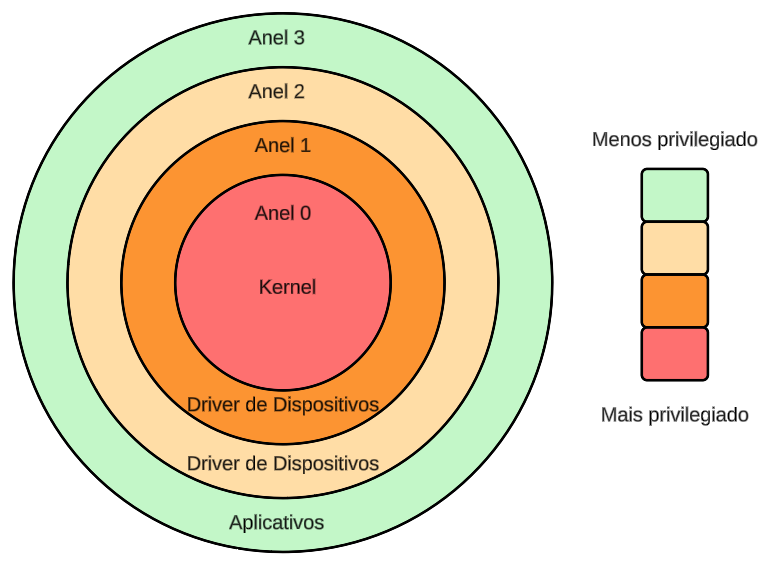
\includegraphics[width=0.7\textwidth]{images/rings_x86.png}
  \label{fig:rings_x86}
\end{figure}

Essa lógica de segurança em formato de anéis ajuda na virtualização e no controle dos hypervisores, os quais explicaremos logo em seguida. Os anéis de nível mais baixo, anel 0, têm acesso aos anéis de nível mais alto, anel 3, mas não vice-versa. O SO realiza a segmentação, um método utilizado para definir diferentes regiões da memória com níveis de privilégio distintos. No Linux e na maioria dos sistemas operacionais modernos, o que mais importa é o anel 3 (user mode), menos privilegiado, e o anel 0 (kernel mode), mais privilegiado (\cite{modernOS}). Os demais anéis também são utilizados para armazenar drivers que precisam de mais privilégio que o modo usuário mas menos do que o kernel.

A interação entre o hardware e o sistema operacional na arquitetura x86-64 é fundamental para garantir a segurança e integridade do sistema. Cada anel de privilégio possui um conjunto específico de instruções que pode executar, e o hardware implementa mecanismos que restringem o acesso a essas instruções de acordo com o nível de privilégio. Por exemplo, o código que roda no anel 3, onde estão as aplicações de usuário, não pode executar diretamente instruções privilegiadas que interagem com o hardware, como manipular registros de controle ou acessar diretamente dispositivos de E/S (entrada/saída) (\cite{chirammal2016mastering}). 

Além disso, o hardware utiliza tabelas de descritores de segmentos e tabelas de páginas para garantir que cada anel tenha acesso apenas às porções de memória designadas para seu nível de privilégio. Esses mecanismos previnem, por exemplo, que um código malicioso em anel 3 tente acessar diretamente áreas de memória que pertencem ao kernel ou a outras aplicações. Dessa forma, a combinação de segmentação, gerenciamento de memória e controle de instruções pelo hardware e SO forma uma barreira eficaz contra violações de segurança ~(\cite{chirammal2016mastering}).



\subsection{Hypervisor ou VMM}

Ao lidarmos com máquinas virtuais (VMs), é essencial contar com um serviço que gerencie essas instâncias de maneira eficiente, permitindo que possamos iniciar, excluir e replicar nossas máquinas de forma organizada. Esse serviço é desempenhado pelo hypervisor, cujo papel é fornecer suporte a múltiplas cópias do hardware físico (\cite{modernOS}). Nos hypervisores modernos, é possível visualizar detalhes de cada VM em execução, como logs, utilização de recursos, tráfego de rede, entre outros aspectos. Além disso, o hypervisor é responsável por definir como a VM será construída e como interagirá com o sistema operacional principal (\cite{chirammal2016mastering}).

O hypervisor desempenha um papel crucial na tradução de chamadas de sistema (syscalls). Quando uma VM executa uma função crítica, não é viável conceder acesso irrestrito ao hardware, devido a questões de escalabilidade e segurança (\cite{modernOS}). Para resolver esse problema, o hypervisor realiza modificações nas chamadas críticas, permitindo que a VM funcione como um sistema operacional principal, conforme ilustrado na Figura \ref{fig:binary_translate} onde temos os serviços separados em aneis com o hypervisor no anel 0 e no anel 1 o sistema operacional reescrevendo os binários antes da execução e fazendo a emulação. Dessa forma, o hypervisor impede que a VM tenha acesso irrestrito ao hardware. Por exemplo, quando a VM tenta acessar diretamente um recurso específico, como a memória, o hypervisor intercepta essa solicitação e a traduz, garantindo a segurança e o controle. Assim, a VM só consegue visualizar o espaço de memória que lhe foi alocado.

\begin{figure}[htbp]
  \centering
  \caption{Tradução de binários em hypervisores. A figura ilustra a separação em anéis de proteção, com o hypervisor operando no anel 0 e o sistema operacional convidado no anel 1. O hypervisor intercepta e reescreve binários críticos antes da execução, realizando a emulação e garantindo a segurança ao evitar o acesso direto ao hardware.}
  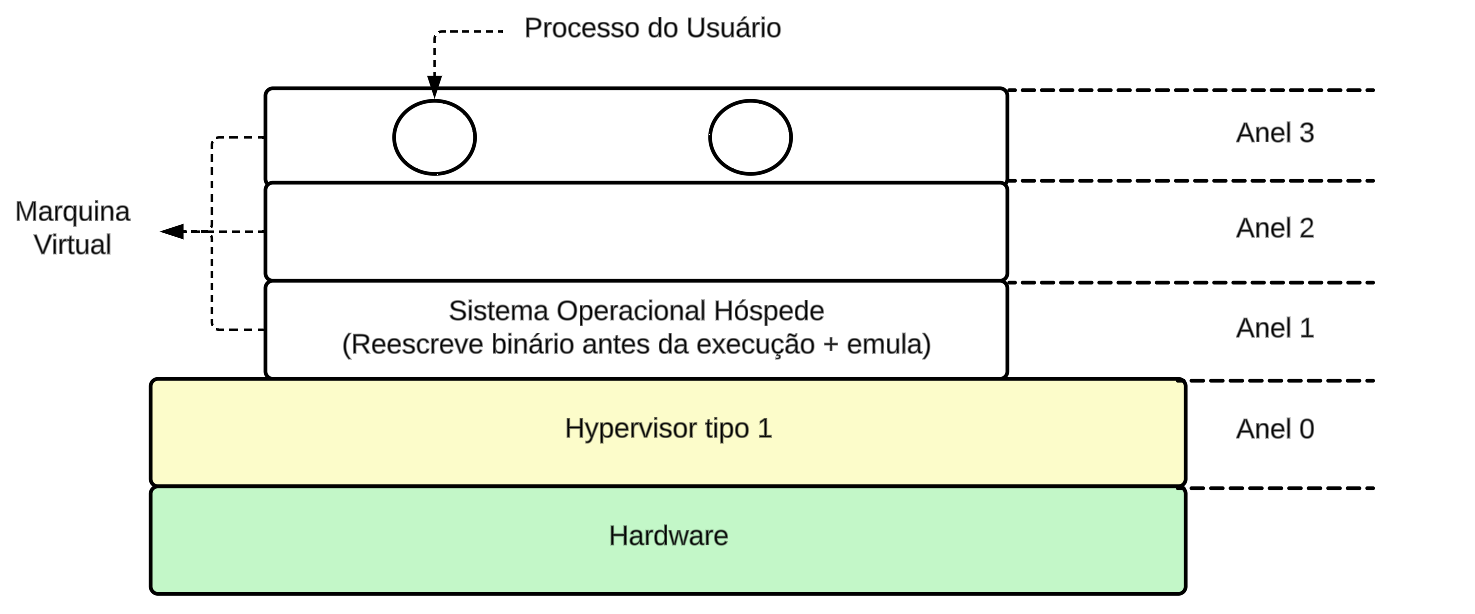
\includegraphics[width=0.7\textwidth]{images/BinaryTranslate.png}
  \caption*{\textit{Fonte:} Adaptado de Modern Operating Systems (\cite{modernOS}).}
  \label{fig:binary_translate}
\end{figure}


As arquiteturas de hypervisores também podem variar bastante de um sistema operacional para outro. No caso do Windows, o hypervisor mais utilizado é o Hyper-V, que também é a solução adotada pela Azure para a implementação de sua infraestrutura como serviço (IaaS) \href{https://learn.microsoft.com/pt-br/azure/architecture/reference-architectures/n-tier/high-security-iaas}. No entanto, nesta pesquisa, nosso foco será no sistema operacional Linux, devido à sua predominância no mercado de servidores (\cite{OperationSystemMarketVolume}) e ao fato de ser open-source (\cite{WhyUseLinux}). Especificamente, abordaremos o hypervisor KVM, que é amplamente utilizado nos principais provedores de IaaS, como AWS e Google.


\subsection{Hypervisor Tipo 1 (Nativo ou Bare Metal)}

A Figura \ref{fig:hypervisor_type01} ilustra o hypervisor tipo 1, que é o mais utilizado quando estamos falando de IaaS, o motivo é que ele opera junto ao hardware, as chamadas críticas são feitas diretas no kernel do OS aumentando sua performance (\cite{chirammal2016mastering}), um exemplo notável é o hypervisor KVM(Kernel-based Virtual Machine) do Linux. Ele consegue transformar kernel do Linux em um hypervisor fazendo com que a VM seja vista como um processo dentro do sistema, como podemos ver na imagem não temos camadas itermediárias para rodar o hypervisor, ele roda junto ao hardware.


\begin{figure}[h!]
  \centering
  \caption{Hypervisor do tipo 1. A imagem ilustra a operação direta com o hardware, onde não há camadas intermediárias entre o hypervisor e o hardware, aumentando a performance.}
  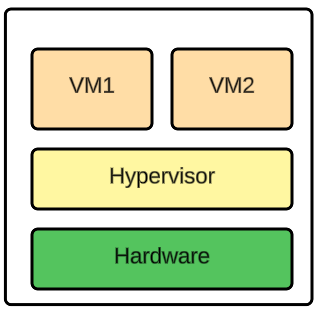
\includegraphics[width=0.4\textwidth]{images/hypervisor_type_1.png}
  \caption*{\textit{Fonte:} Adaptado de (\cite{chirammal2016mastering}).}
  \label{fig:hypervisor_type01}
\end{figure}



Perceba que no bare metal não temos a ideia de um host OS, o hypervsior está direto com o hardware porque roda junto ao kernel.


\subsection*{Hypervisor Tipo 2 (Hospedeiro)}

O hypervisor tipo 2, mostrado na figura \ref{fig:hypervisor_type02}, requer um sistema operacional host principal para funcionar, sendo útil pela facilidade de manuseio e instalação. No entanto, ele não é a melhor opção quando se necessita de alta performance e escalabilidade. Isso se deve, claramente, às camadas adicionais de software que ele introduz. Diferentemente de um hypervisor bare metal, o hypervisor hospedeiro gera uma sobrecarga maior por operar dentro de um sistema operacional, resultando em chamadas de sistema que são intermediadas pelo \textit{host OS}. Essa configuração cria uma camada de abstração adicional, que pode reduzir a eficiência nas operações críticas.


\begin{figure}[htbp]
  \centering
  \caption{Hypervisor do tipo 2. A imagem mostra a necessidade de um sistema operacional hospedeiro para o funcionamento do hypervisor.}
  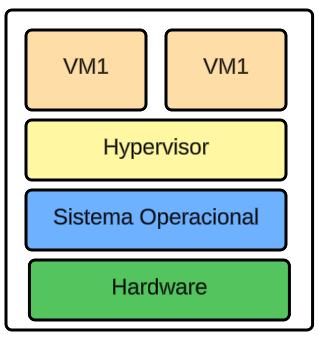
\includegraphics[width=0.4\textwidth]{images/hypervisor_type_2.png}
  \caption*{\textit{Fonte:} Adaptado de (\cite{chirammal2016mastering}).}
  \label{fig:hypervisor_type02}
\end{figure}


Neste caso o hypervisor e visto de fato como um serviço a parte que está executando no sitema operacional e a VM será vista como um filho desse serviço.


\section{Virtualizações}

Existem três grandes formas de efetuar a virtualização por meio do hypervisor, cada uma utilizando características específicas que podem ser aplicadas em diferentes cenários.

\subsection{Virtualização Completa (Full Virtualization)}

Neste método, o hypervisor emula o hardware para permitir que o sistema operacional convidado (\textit{Guest OS}) opere como se estivesse em uma máquina física independente como monstrado na figura \ref{fig:full_virtualization_rings}. Não há necessidade de modificações no sistema operacional convidado, pois ele não sabe que está sendo virtualizado. Praticamente todas as funções são traduzidas pelo hypervisor, evitando chamadas diretas da VM para o kernel do host. O \textit{Guest OS} roda no anel 1, enquanto a máquina virtual (\textit{Virtual Machines Monitor} - VMM) roda no anel 0 (\cite{chirammal2016mastering}).

\begin{figure}[htbp]
  \centering
  \caption{Virtualização completa nos anéis de segurança. A figura demonstra o \textit{Guest OS} operando no anel 1 e o VMM no anel 0, com o hypervisor realizando a emulação.}
  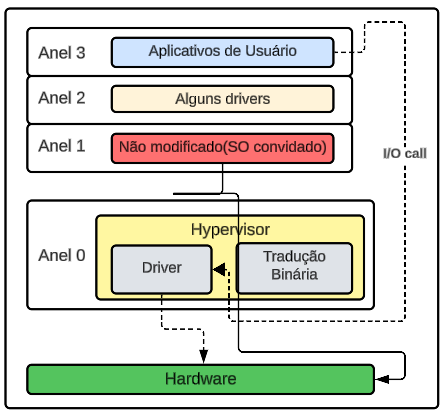
\includegraphics[width=0.7\textwidth]{images/full_virtualization_rings.png}
  \caption*{\textit{Fonte:} Adaptado de (\cite{chirammal2016mastering}).}
  \label{fig:full_virtualization_rings}
\end{figure}


Esse estilo de virtualização utiliza o mecanismo \textit{Trap and Emulate} (Armadilha e Emulação). Quando o \textit{Guest OS} tenta acessar um endereço de memória indevido, o acesso é capturado e emulado pelo hypervisor (\cite{chirammal2016mastering}), o que pode gerar uma sobrecarga maior no sistema.

\subsection{Paravirtualização}

Nesse caso, o \textit{Guest OS} é modificado para interagir diretamente com o hypervisor, resultando em um desempenho melhor em comparação à virtualização completa. As instruções sensíveis são removidas, e, em vez disso, o sistema operacional realiza chamadas diretas ao hypervisor para operações como E/S e mudanças em registros críticos, similar a como programas de aplicação fazem chamadas de sistema em Linux (\cite{modernOS}).

A figura \ref{fig:paravirtualization_rings} mostra como o SO convidado modificado realiza chamadas críticas diretamente para o hypervisor por meio de hypercalls. Como o SO foi adaptado para trabalhar nesse ambiente, o tratamento de chamadas sensíveis se torna mais eficiente, reduzindo a necessidade de simulação todas as instruções.

\begin{figure}[htbp]
  \centering
  \caption{Paravirtualização nos anéis de segurança. A figura mostra como o sistema operacional convidado modificado realiza chamadas críticas diretamente para o hypervisor por meio de hypercalls, tornando o tratamento mais eficiente e reduzindo a necessidade de emulação.}
  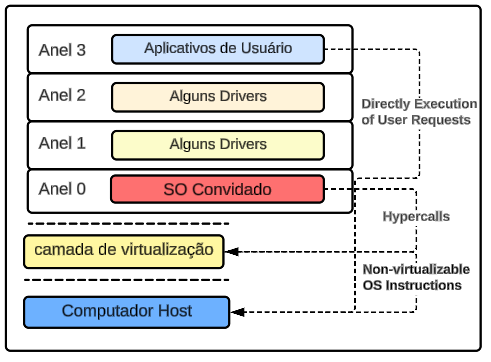
\includegraphics[width=0.7\textwidth]{images/paravirtualization_rings.png}
  \caption*{\textit{Fonte:} Adaptado de (\cite{chirammal2016mastering}).}
  \label{fig:paravirtualization_rings}
\end{figure}

O \textit{Guest OS} opera no anel zero, aproveita as modificações nas chamadas críticas e evitar ações indevidas para reduzir a sobrecarga tornando mais performático que a virtualização completa.

\subsection{Virtualização Assistida por Hardware}

A forma mais eficiente de virtualização é a assistida por hardware, que utiliza recursos nativos do processador, como \textit{Intel VT-x} ou \textit{AMD-V}, para executar funções de virtualização diretamente no hardware. Além disso, funções nativas do kernel Linux podem ser utilizadas para otimizar o controle das VMs (\cite{chirammal2016mastering}). Quando uma instrução sensível é executada, o hardware captura a operação e a passa ao hypervisor para emulação (\cite{modernOS}).

A figura \ref{fig:hardware_assisted_rings} apresenta uma visão esquemática dos diferentes anéis de privilégio utilizados na virtualização assistida por hardware. Nela, o \textit{Guest OS} opera no anel zero, o mesmo nível de privilégio em que um sistema operacional tradicional funcionaria em uma máquina física, enquanto o hypervisor assume um papel central no anel -1, criado especificamente para gerenciar diretamente o acesso ao hardware. Essa estrutura permite que o hypervisor intercepte chamadas sensíveis e controle os recursos de forma eficiente, enquanto o sistema convidado e suas aplicações continuam a operar como se tivessem controle completo sobre o hardware subjacente.

\begin{figure}[htbp]
  \centering
  \caption{Virtualização assistida por hardware nos anéis de segurança. A figura mostra o \textit{Guest OS} operando no anel 0 e o hypervisor no anel -1, permitindo um gerenciamento eficiente do hardware e reduzindo a necessidade de emulação por software.}
  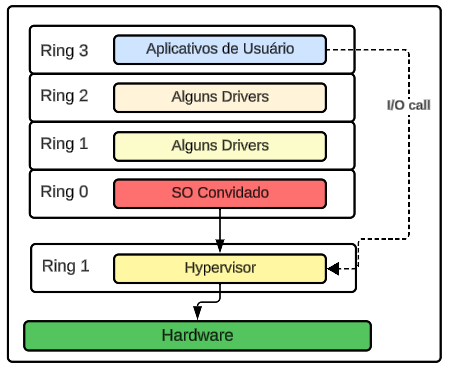
\includegraphics[width=0.7\textwidth]{images/hardware_assisted_rings.png}
  \caption*{\textit{Fonte:} Adaptado de (\cite{chirammal2016mastering}).}
  \label{fig:hardware_assisted_rings}
\end{figure}

A virtualização assistida por hardware se destaca pela eficiência porquê o processador fica responsável por lidar diretamente com operações sensíveis, eliminando a necessidade de emular essas instruções no software. Essa abordagem reduz a latência associada às traps e minimiza o impacto no desempenho causado pela invalidação de caches e TLBs. O uso de anéis de privilégio dedicados, como o anel -1 para o hypervisor, permite que os sistemas convidados operem de forma isolada e com alta performance, enquanto o hypervisor gerencia as interações críticas com o hardware de maneira otimizada (\cite{chirammal2016mastering}).

\subsection{Considerações sobre os tipos de virtualização}

Não são apenas as funções críticas que são traduzidas pelo hypervisor. Utilizando a tecnologia VT (Virtualization Technology), o hardware gera uma grande quantidade de interrupções, conhecidas como traps. Essas traps podem prejudicar significativamente o desempenho do sistema, pois invalidam o cache da CPU e os TLBs (Translation Lookaside Buffers), que são ewssenciais para o rápido acesso à memória. Quando o cache e os TLBs são invalidados, a CPU precisa recarregar essas informações, o que aumenta a latência e reduz a eficiência geral. Para mitigar esses efeitos negativos, o hypervisor captura e traduz algumas funções não críticas. Isso é feito para reduzir a frequência das traps e, consequentemente, diminuir o impacto sobre o desempenho. Ao gerenciar melhor quais funções precisam ser interceptadas e traduzidas, o hypervisor pode manter um equilíbrio entre a funcionalidade e a eficiência do sistema (\cite{modernOS}).

Lembrando que essas 3 são formas gerais de virtualização, como serão feitas as traduções binárias das funções críticas a emulação entre outros detalhes vai depender do hypervisor que está sendo utilizado. Nenhuma instrução sensível emitida pelo sistema operacional hóspede jamais é executada diretamente pelo verdadeiro hardware. Elas são transformadas em chamadas pelo hipervisor, que então as emula (\cite{modernOS}).

Como estamos falando que computação em nuvem privada nosso foco vai ser o hypervisor do tipo 1 e com a virtualização assistida pelo hardware utilizado pelo OpenStack, o mótivo dessa escolha é pelos detalhes que falamos a cima, precisamos do máximo de performace possível e alta escalabilidade, o OpenStack aceita vários tipos de hypervisors mas por padrão é utilizado o QEMU/KVM (\cite{DocumentacaoOpenstack}).


\section{Importância das Tecnologias de Virtualização para VMs}

Tecnologias como o KVM (Kernel-based Virtual Machine) e ferramentas como o Libvirt proporcionam uma base robusta para a criação, gerenciamento e escalabilidade de VMs, enquanto a virtualização assistida por hardware e técnicas de alocação de recursos (CPU, memória e rede) garantem que as VMs operem com alto desempenho. Estas tecnologias são indispensáveis para qualquer infraestrutura moderna que dependa de VMs para suportar suas operações e demandas em ambientes complexos e de larga escala.

\subsection{Libvirt - API e VMs}
O \textit{libvirt} é amplamente utilizado em diversos serviços que gerenciam máquinas virtuais (VMs), sendo uma biblioteca essencial para simplificar a criação e administração dessas VMs. Ele oferece uma interface unificada e de fácil utilização para diferentes tecnologias de virtualização, como o \textit{QEMU}, que, por sua vez, utiliza o \textit{KVM} para aproveitar a aceleração por hardware. Além disso, o \textit{OpenStack}, por meio do serviço \textit{NOVA}, utiliza o \textit{libvirt} para a orquestração de VMs (\cite{DocumentacaoOpenstack}) \href{https://docs.openstack.org/kolla-ansible/latest/reference/compute/libvirt-guide.html}{libvirt guide}.

Um exemplo de criação de uma máquina virtual utilizando o \textit{libvirt} com \textit{QEMU-KVM} pode ser feito através do comando \texttt{virt-install} diretamente no terminal, passando os parâmetros de configuração desejados. Esses parâmetros são convertidos em um arquivo XML que descreve as especificações da VM. Esse arquivo, geralmente localizado em \texttt{/etc/libvirt/qemu}, pode ser editado manualmente conforme necessário. O \textit{QEMU}, em conjunto com o \textit{KVM}, utiliza essas informações para configurar e iniciar a máquina virtual de maneira otimizada. Por padrão, se o KVM estiver disponível no sistema, ele será utilizado para melhorar o desempenho da VM.

O \textit{libvirt} é, na verdade, um conjunto de APIs chamado ``Virtualization API'', que permite o gerenciamento padronizado de várias plataformas de virtualização, como \textit{KVM}, \textit{QEMU}, \textit{Xen}, \textit{VMware}, \textit{Hyper-V}, e \textit{LXC}. Essas APIs fornecem uma camada de abstração, permitindo que diferentes hipervisores sejam controlados de maneira uniforme e consistente (\cite{chirammal2016mastering}). Isso torna o \textit{libvirt} uma ferramenta central em ambientes de virtualização complexos e escaláveis.

Como mostrado da figura \ref*{fig:libvirt_interface}, ele utiliza dos driver de cada hypervisor, os drivers são descobertos durante o processo de conexão com a API. Cada driver tem uma API de registro que carrega as referências de função específicas do driver para as APIs libvirt chamarem, assim como os respectivos protocolos utilizados por essas APIs. A arquitetura do driver também é usada para dar suporte a outros componentes de virtualização, como armazenamento, pools de armazenamento, dispositivo host, rede, interfaces de rede e filtros de rede \url{https://libvirt.org/api.html}. Um exemplo simples de XML configurado para 1 vCPU utilizando o KVM e o QEMU, armazenando a imagem no arquivo do tipo QCOW2 pode ser visto em (Código \ref{code:example_kvm_qemu})


\begin{figure}[htbp]
  \centering
  \caption{Interface para drivers do \textit{libvirt}. A figura ilustra como o \textit{libvirt} se conecta a diferentes hypervisores por meio de drivers específicos, permitindo o gerenciamento padronizado de componentes de virtualização, como rede, armazenamento e dispositivos.}
  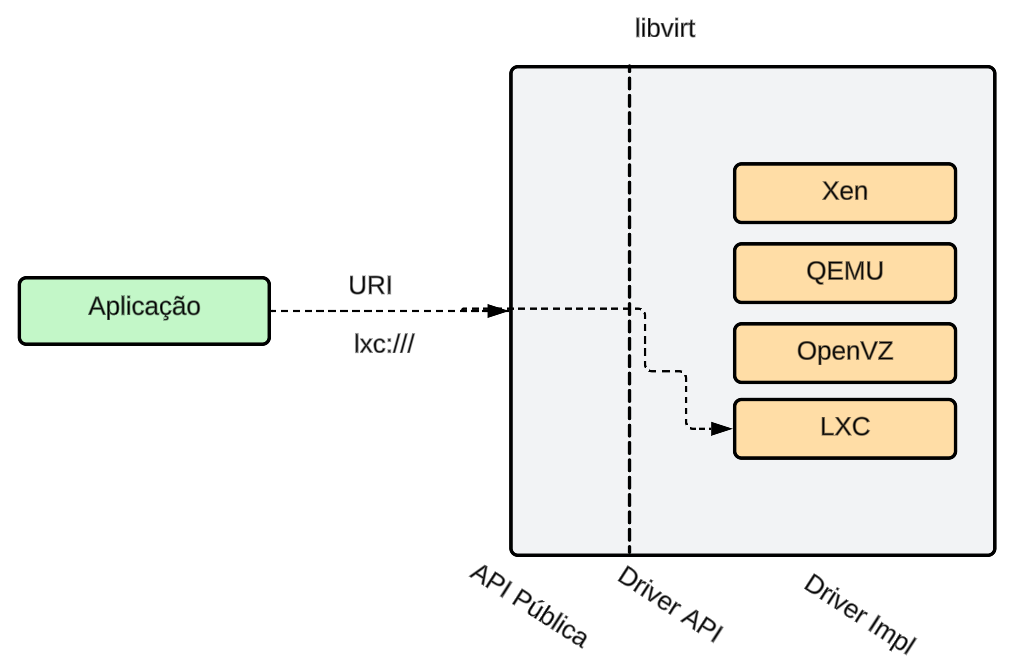
\includegraphics[width=0.7\textwidth]{images/libvirt_interface.png}
  \caption*{\textit{Fonte:} Adaptado de \url{https://libvirt.org/api.html}.}
  \label{fig:libvirt_interface}
\end{figure}

\begin{listing}[h!]
  \noindent\fcolorbox{black}{gray!10}{%
  \parbox{\textwidth}{%
    \inputminted[]{xml}{files/example.xml}
  }%
}  
\caption{Exemplo de configuração em XML para uma VM utilizando \textit{KVM} e \textit{QEMU}. O arquivo define as especificações da máquina virtual, incluindo uma vCPU, memória, tipo de armazenamento em formato QCOW2, e outras configurações essenciais para a inicialização e operação da VM.}
\label{code:example_kvm_qemu}
\end{listing}


Este código contém as informações necessárias para configurar a VM, incluindo a memória, quantidade de vCPUs, imagem de carregamento, tipo de arquivo, entre outras configurações.

Naturalmente, para salvar o storage das VMs, utilizamos o arquivo QCOW2 (QEMU Copy On Write version 2). Ele possui diversas funcionalidades que ajudam no manuseio das imagens e na escalabilidade. Sua estrutura foi desenhada pelo QEMU pensando no manuseio de VMs, por isso inclui recursos como snapshots, compressão, encriptação e redimensionamento dinâmico.


\subsection{KVM - Kernel-based Virtual Machine}

O \textbf{Kernel-based Virtual Machine (KVM)}, como comentado acima, interage com o kernel para formar um poderoso hipervisor tipo 1 para sistemas operacionais baseados em Linux, amplamente utilizado em serviços de nuvem. Ele permite a orquestração de VMs com funções integradas diretamente ao kernel e oferece virtualização assistida por hardware.

O KVM não funciona como um serviço independente, ele precisa estar integrado ao kernel do Linux e depende da assistência de hardware para virtualização \textit{(VT-X)}, utilizando módulos específicos como os encontrados em \textit{kvm-intel.ko}. Além disso, o KVM também precisa do \textbf{QEMU}, que fornece os binários necessários para a construção e gerenciamento das VMs. Juntos, KVM e QEMU formam um hipervisor robusto, capaz de controlar várias VMs, oferecendo uma solução de virtualização escalável e eficiente (\cite{chirammal2016mastering}).

De forma geral, o módulo de kernel do KVM é responsável por diversas funções críticas (\cite{chirammal2016mastering}):

\begin{itemize}
    \item \textbf{Gestão de CPUs Virtuais (vCPUs)}: O KVM gerencia vCPUs, que são \textit{threads} POSIX criadas para cada VM, permitindo a execução de instruções diretamente no kernel do sistema operacional.
  
    \item \textbf{Gerenciamento de Memória}: Utiliza \textit{EPT} (Extended Page Tables) ou \textit{NPT} (Nested Page Tables) para gerenciar a memória alocada para cada VM, assegurando o mapeamento eficiente entre a memória virtual da VM e a memória física do host.

    \item \textbf{Manuseio de \textit{Threads} de I/O}: Facilita a comunicação entre dispositivos virtuais e o hardware físico, interceptando e encaminhando operações de I/O.

    \item \textbf{Interrupções e Exceções}: Lida com interrupções e exceções geradas por chamadas críticas, utilizando virtualização assistida por hardware para emular respostas apropriadas.

    \item \textbf{Controle e Monitoramento}: Expondo uma interface por meio de \textit{ioctls}, o KVM permite a configuração, controle e monitoramento das VMs.

    \item \textbf{Segurança e Isolamento}: Garante a segurança e o isolamento das VMs, controlando o acesso a cada espaço de memória e evitando interferências entre as VMs.
\end{itemize}

Na figura \ref{fig:qemu_kvm_architecture}, é ilustrada a arquitetura do hipervisor QEMU/KVM, mostrando como o QEMU e o KVM interagem para emular uma virtualização, gerenciar vCPUs e realizar transições entre os modos do host e do convidado. Na seção superior, o modelo de máquina virtual exibe componentes como o subsistema de E/S e os threads da CPU responsáveis pela execução das instruções da VM. Já a seção inferior destaca o papel do KVM, que utiliza APIs específicas e tabelas de páginas estendidas (\textit{EPT}) para gerenciar memória e executar VMs em modo convidado, enquanto monitora eventos de saída (\textit{VM Exit}) e lida com interrupções, entradas/saídas e violações de página. Essa integração entre QEMU e KVM resulta em uma infraestrutura robusta para virtualização assistida por hardware, assegurando desempenho e isolamento entre as VMs.

\begin{figure}[htbp]
  \centering
  \caption{Arquitetura do hypervisor QEMU/KVM. A figura ilustra a interação entre o QEMU e o KVM, mostrando o gerenciamento de vCPUs, E/S e memória, além das transições entre o modo do host e do convidado para virtualização assistida por hardware.}
  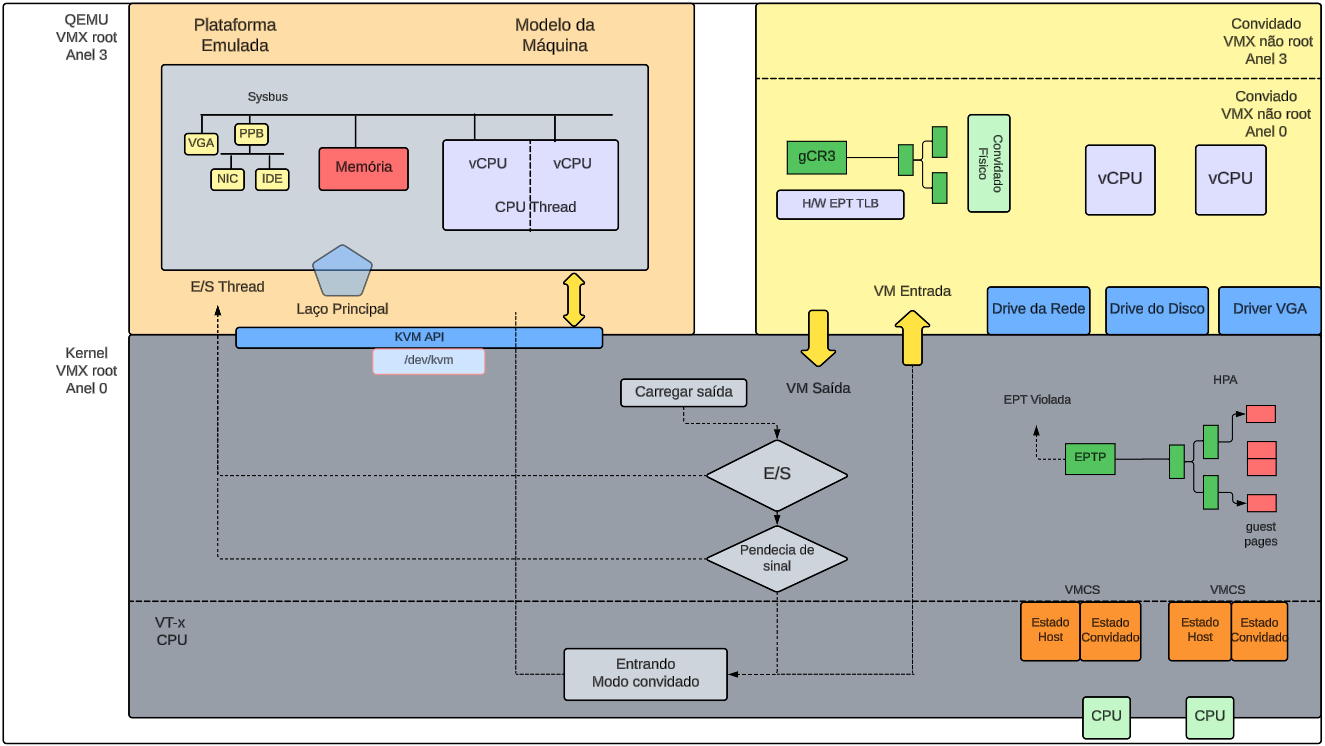
\includegraphics[width=0.9\textwidth]{images/qemu_kvm_architecture.png}
  \caption*{\textit{Fonte:} Adaptado de \url{https://wiki.qemu.org/Documentation/Architecture}.}
  \label{fig:qemu_kvm_architecture}
\end{figure}


\subsection{VMX para o KVM}

O \textbf{VMX} é substancial para o \textbf{KVM}, que utiliza as funções \textit{VM*} disponibilizadas pela tecnologia de hardware assistido. Essas funções são usadas para o controle da VM e são disponibilizadas pelo \textbf{KVM} para que outros serviços de mais alto nível possam acessá-las através dos \textit{ioctls} (input/output control) (\cite{wiki:Ioctl}), que ficam em \textit{/dev/kvm}. Alguns exemplos de funções disponibilizadas pelo hardware são:

\begin{itemize}
  \item \textbf{VMREAD}: Lê o conteúdo de um campo de controle específico da VM.
  \item \textbf{VMWRITE}: Escreve um valor em um campo de controle específico da VM.
  \item \textbf{VMCLEAR}: Limpa a estrutura da VM.
  \item \textbf{VMPTRLD}: Carrega o ponteiro para a estrutura da VM.
  \item \textbf{VMLAUNCH}: Inicia a execução da VM.
  \item \textbf{VMRESUME}: Retoma a execução da VM após uma interrupção.
\end{itemize}

Essas funções interagem com o KVM através de chamadas ao \textit{ioctl}. O \textbf{KVM} fornece uma interface que os usuários podem utilizar para configurar e controlar VMs, e essa interface faz uso das funções VMX para manipular diretamente o estado e a execução das VMs no nível do hardware (\cite{zabaljauregui2008hardware}). Existem diversas outras chamadas que são utilizadas.

Essa relação é de extrema importância para o \textbf{QEMU-KVM}, pois o \textbf{QEMU} utiliza as chamadas \textit{ioctls} disponibilizadas na interface do KVM para se comunicar com o hardware de maneira mais eficiente.

\subsection{Alocação de CPU}

Como comentado, uma vCPU, que é a CPU da VM, é implementada como uma \textit{thread} POSIX. Isso significa que ela funciona como uma conexão ao CPU físico, com funções que ajudam a controlá-la. Essas \textit{threads} são semelhantes a qualquer outra \textit{thread} no sistema operacional \textit{host} em termos de execução (\cite{chirammal2016mastering}).

A forma como cada vCPU será processada depende de como o escalonador do Linux irá tratá-la. O escalonador do Linux gerencia a alocação de tempo de CPU para todas as \textit{threads}, incluindo aquelas que representam vCPUs. Em geral, podemos esperar uma média de 2 \textit{threads} vCPU para cada núcleo físico da CPU, embora isso possa variar dependendo da aplicação e do hardware utilizado (\cite{TechTargetvCPU}).

\subsection{Alocação de Memória}

A alocação de memória é uma parte crítica no processo de criação e gerenciamento de máquinas virtuais (VMs). Cada VM precisa de sua própria área de memória para operar, e o gerenciamento dessa memória é essencial para garantir que o sistema \textit{host} possa suportar múltiplas VMs simultaneamente sem sobrecarregar os recursos disponíveis. De forma geral, cada VM possui suas próprias tabelas de páginas que mapeiam endereços de memória virtual para endereços de memória física (\cite{modernOS}).

No contexto de sistemas como QEMU/KVM, por exemplo, a alocação de memória envolve a leitura de um arquivo de configuração (como um XML) que especifica a quantidade de memória necessária para a VM. A memória especificada é então reservada no espaço de endereço do processo, e o \textit{hypervisor} (KVM, neste caso) é responsável por criar as páginas de memória necessárias para traduzir os endereços de memória virtual da VM para a memória física do \textit{host} (\cite{chirammal2016mastering}).

\subsection{Virtualização na Placa de Rede}

Para que todas as VMs de uma máquina tenham acesso a uma rede, precisamos de três componentes principais: \textit{Hypervisor}, NICs virtuais (\textit{Network Interface Controller}) e os Switches Virtuais. Cada VM possui sua própria vNIC com endereço MAC (\textit{Media Access Control}) e IP (\textit{Internet Protocol}) próprios. 

O \textit{switch} virtual (vSwitch) é um componente essencial que permite a comunicação entre as vNICs e a NIC real. Ele funciona como um \textit{switch} normal, encaminhando pacotes entre as vNICs e a rede física, permitindo que todas consigam se comunicar.

O \textbf{SR-IOV} (\textit{Single Root I/O Virtualization}) é outra tecnologia importante para a virtualização. Ele permite que uma única NIC física apresente múltiplas interfaces lógicas, como mostrado na figura \ref{fig:single_root_IO_virtualization}. Cada interface lógica é chamada de \textit{Virtual Function} (VF). Naturalmente, cada VF é atribuída a uma VM, permitindo acesso direto ao hardware da NIC, melhorando a performance (\cite{dong2012high}), enquanto a \textit{Physical Function} (PF) compartilha recursos com as VFs.

\begin{figure}[htbp]
  \centering
  \caption{Arquitetura SR-IOV. A figura ilustra como uma única NIC física pode apresentar múltiplas interfaces lógicas (\textit{Virtual Functions} - VFs), permitindo que cada VM tenha acesso direto ao hardware, enquanto a \textit{Physical Function} (PF) gerencia os recursos compartilhados.}
  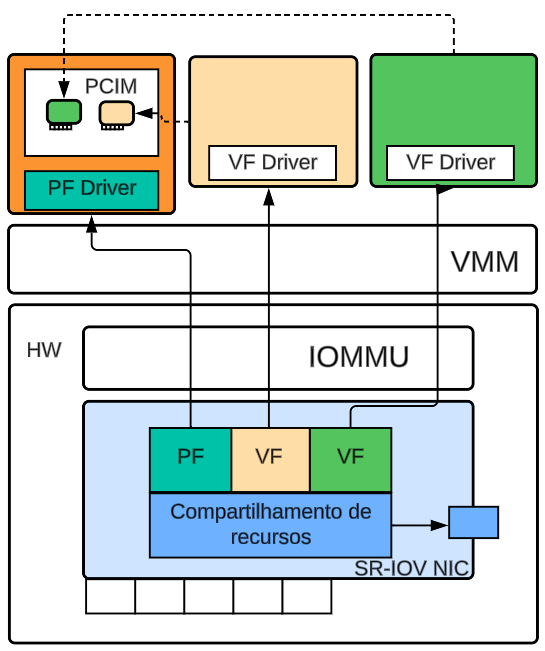
\includegraphics[width=0.5\textwidth]{images/single_root_IO_virtualization.png}
  \caption*{\textit{Fonte:} Adaptado de (\cite{dong2012high}).}
  \label{fig:single_root_IO_virtualization}
\end{figure}


Junto a todas essas tecnologias, utilizamos também algoritmos para efetuar o balanceamento de carga, como \textit{Round-Robin}, \textit{Least Connections} e \textit{Weighted Fair Queuing}, usados para distribuir o tráfego de maneira eficiente entre várias VMs (\cite{dong2012high}).


\section{Containers}

Container é uma forma leve de virtualização que permite isolar processos e seus recursos em um ambiente controlado e consistente. Os containers compartilham o mesmo \textit{kernel} do sistema operacional, mas são isolados uns dos outros e do sistema \textit{host}, proporcionando uma maneira eficiente de executar aplicações com suas dependências em um ambiente previsível.

O \textbf{LXC} (\textit{Linux Containers}) foi a primeira grande implementação dos containers como conhecemos hoje em dia (\cite{HistoryOfCloudByIBM}), um serviço isolado executando com uma certa limitação de hardware e de fácil criação. Esse novo sistema serviu de inspiração para o desenvolvimento de grandes serviços usados na indústria hoje em dia, como o \textbf{Docker}.

De forma geral, os containers são criados utilizando tecnologias existentes dentro do sistema operacional. No caso dos sistemas baseados em \textit{Unix}, utilizam-se as tecnologias de \textit{namespaces} e \textit{cgroups}. Iremos destacar melhor como cada uma dessas tecnologias funciona, mas, basicamente, utilizamos essas tecnologias para fazer a limitação de recursos e separação de acesso lógico.

Quando comparamos a infraestrutura necessária para executar uma VM ou um container, percebemos que, de fato, ocorre uma diminuição de \textit{overhead}. A VM precisa de emulação de hardware, enquanto o container é apenas software (\cite{OCIContainer}), como mostrado na figura \ref{fig:vm_x_container}. No caso dos containers, eles também compartilham o mesmo \textit{host kernel}, o que gera maior facilidade na hora de escalar a quantidade de containers.


\begin{figure}[htbp]
  \centering
  \caption{Comparação de arquitetura entre containers e VMs. A figura mostra como os containers compartilham o \textit{kernel} do host, enquanto as VMs utilizam um hypervisor e requerem emulação de hardware, resultando em maior \textit{overhead} para VMs.}
  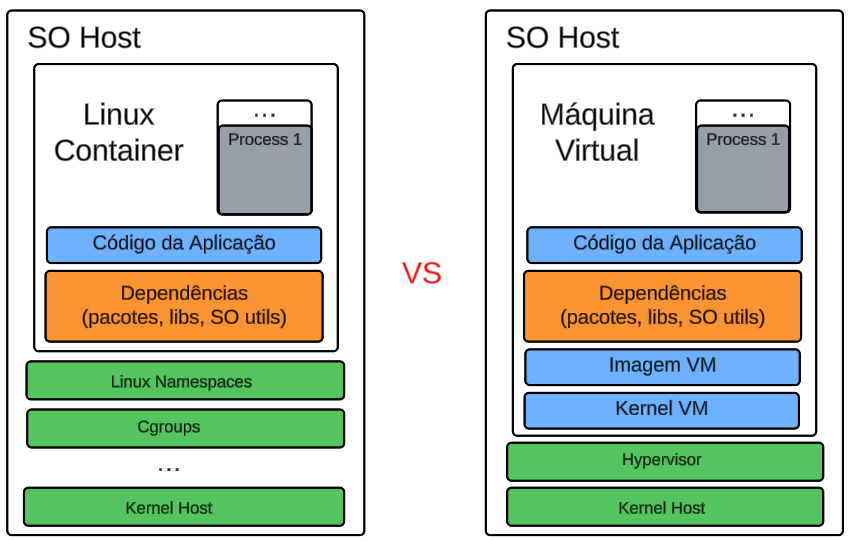
\includegraphics[width=0.7\textwidth]{images/vm_x_container_2.png}
  \caption*{\textit{Fonte:} Adaptado de (\cite{OCIContainer}).}
  \label{fig:vm_x_container}
\end{figure}


\subsection{Namespaces}

Atualmente, o Linux implementa sete tipos diferentes de \textit{namespaces}. O propósito de cada \textit{namespace} é encapsular um recurso de sistema global específico em uma abstração que faz parecer aos processos dentro do \textit{namespace} que eles têm sua própria instância isolada do recurso global. Um dos objetivos gerais dos \textit{namespaces} é dar suporte à implementação de containers, uma ferramenta para virtualização leve (bem como outros propósitos) que fornece a um grupo de processos a ilusão de que eles são os únicos processos no sistema (\cite{LWNNamespaces}).

Existem \textit{namespaces} essenciais no Linux, cada um com uma tarefa importante no sistema operacional para garantir segurança e isolamento:

\begin{itemize}
  \item \textbf{PID (Identificador de Processo):} Isola os IDs de processos. Dessa forma, processos dentro do \textit{namespace} PID não podem ver processos de fora dele. Isso significa que processos com \textit{namespaces} diferentes podem ter o mesmo PID, porém não têm visibilidade ou interferência uns com os outros. Funciona como um serviço hierárquico: o processo pai tem acesso ao filho, mas isso também pode ser alterado, isolando completamente o processo filho.
  
  \item \textbf{NET (Rede):} Isola interfaces de rede, roteadores, tabelas de roteamento, \textit{firewalls} e \textit{sockets} de rede, permitindo um isolamento completo da rede. Isso significa que cada \textit{namespace} de rede pode ter suas próprias interfaces de rede, rotas, regras de \textit{firewall}, etc., sem interferir nos \textit{namespaces} de rede de outros processos. É frequentemente usado para criar ambientes de rede virtualizados, como containers com suas próprias pilhas de rede.
  
  \item \textbf{MNT (Montagem de Sistemas de Arquivos):} Isola a árvore de sistemas de arquivos montados. Dessa forma, os processos dentro de um \textit{namespace} de montagem têm uma visão diferente dos sistemas de arquivos montados em comparação aos processos fora desse \textit{namespace}. Isso permite ter diferentes sistemas de arquivos ou pontos de montagem visíveis para diferentes processos. Por exemplo, pode-se montar um diretório somente leitura dentro de um container sem afetar o resto do sistema.
  
  \item \textbf{UTS (Identificação do Sistema):} Isola o nome do \textit{host} e o domínio do sistema. Isso permite que cada \textit{namespace} tenha seu próprio nome de \textit{host} e domínio, possibilitando a criação de ambientes isolados que podem parecer sistemas diferentes para os processos dentro deles. É útil para ambientes de teste e desenvolvimento onde diferentes configurações de nome de \textit{host} são necessárias.
  
  \item \textbf{IPC (Comunicação entre Processos):} Isola recursos de IPC, como filas de mensagens, semáforos e memória compartilhada. Isso garante que os processos dentro de um \textit{namespace} de IPC não possam acessar os recursos de IPC fora dele. Esse isolamento é essencial para containers e outros ambientes de virtualização, onde os recursos de IPC precisam ser isolados para garantir a segurança e a estabilidade.
  
  \item \textbf{USER (Identificação do Usuário):} Isola os IDs de usuário e grupos. Isso permite que processos dentro de um \textit{namespace} de usuário tenham uma visão diferente dos IDs de usuário e grupos comparados aos processos fora do \textit{namespace}. É particularmente útil para permitir que processos dentro de containers rodem como \textit{root} dentro do container, mas como um usuário não privilegiado no sistema \textit{host}, aumentando a segurança.
  
  \item \textbf{CGROUP (Grupos de Controle):} Isola a hierarquia de \textit{cgroups}, usados para limitar e isolar o uso de recursos como CPU, memória, disco e rede. Cada \textit{namespace} de \textit{cgroup} pode ter suas próprias regras e limitações, permitindo a alocação e gerenciamento de recursos de forma eficiente e segura. É uma ferramenta essencial para a gestão de recursos em ambientes de containers e virtualização, garantindo que um container não possa monopolizar os recursos do sistema.
\end{itemize}

\subsection{Cgroups}

Os \textit{cgroups}, como mencionado anteriormente, são essenciais para o gerenciamento de recursos da máquina. Eles permitem definir quanto cada processo pode utilizar, complementando o isolamento oferecido pelos \textit{namespaces}. Enquanto os \textit{namespaces} oferecem isolamento lógico, os \textit{cgroups} garantem o isolamento de recursos. Na prática, containers como Docker e LXC possuem funcionalidades adicionais, mas a base deles é o isolamento lógico e de recursos.

Podemos separar diferentes recursos existentes na máquina utilizando o PID do processo. Sempre que um novo processo é iniciado, o sistema operacional atribui um PID, essencial para a identificação no contexto apropriado \href{https://docs.kernel.org/admin-guide/cgroup-v1/cgroups.html}. Existe um diretório padrão para separar os \textit{cgroups}: \texttt{/sys/fs/cgroup/resource}, onde \texttt{resource} representa o recurso a ser isolado.

Para criar um \textit{cgroup} específico, utilizamos o diretório padrão e adicionamos uma nova pasta com o nome do \textit{cgroup}, por exemplo: \texttt{/sys/fs/cgroup/newgroup/resource}. Dentro desta pasta, configuramos como queremos limitar os recursos. Após essa configuração, basta mover o PID para dentro desse novo \textit{cgroup} na pasta \texttt{/tasks}. Nos novos sistemas operacionais baseados em Linux, é utilizado o \textit{cgroup v2}, que altera um pouco a organização dos diretórios; por exemplo, o PID deve ser movido para \texttt{/newgroup/cgroup.procs}. O (Código \ref{code:debian_docker}) mostra um exemplo de como poderíamos baixar o OS Debian simples apenas com os arquivos necessários para executar o sistema e isolá-lo.


\begin{listing}[h!]
  \noindent\fcolorbox{black}{gray!10}{%
  \parbox{\textwidth}{%
  \inputminted[]{sh}{files/container.sh}
  }%
}  
\caption{Exemplo de script para baixar uma versão mínima do sistema operacional Debian, configurá-lo de forma isolada utilizando \textit{cgroups} e \textit{namespaces}, e executar processos dentro desse ambiente isolado, simulando um container.}
\label{code:debian_docker}
\end{listing}


Após a criação feita no (Código \ref{code:debian_docker}), você já pode executar o serviço isolado como um container. Os containers executados por LXC ou Docker possuem diversas outras \textit{features} que ajudam em uma boa integração para microserviços e automatização de \textit{deploy}, isso é apenas um exemplo.

\subsection{Docker}

O \textbf{Docker} é uma plataforma amplamente utilizada para criar, implantar e gerenciar containers, especialmente em contextos de microserviços e escalabilidade horizontal. Ele facilita a criação de ambientes isolados e consistentes para a execução de aplicativos, utilizando a tecnologia de containers junto com diversas outras funcionalidades (\cite{DockerDocumentation}). O Docker foi desenvolvido com base na tecnologia \textbf{Linux Containers (LXC)}.

Uma das principais inovações do Docker foi a implementação do conceito de imagens dentro dos containers, o que simplificou a cópia e reconstrução de ambientes. Imagens de containers são configurações pré-definidas que podem ser utilizadas para criar ambientes de execução idênticos em qualquer lugar (\cite{DockerDocumentation}). Quando uma imagem é copiada e executada, o Docker constrói um ambiente isolado que replica exatamente a configuração daquela imagem. Essa funcionalidade é extremamente útil para desenvolvedores que precisam garantir a replicação precisa de ambientes de desenvolvimento, teste ou produção.

\subsection{Linux Containers - LXC}  
O \textbf{Linux Containers (LXC)} é uma tecnologia de virtualização a nível de sistema operacional que permite a criação de múltiplas instâncias isoladas de ambientes de usuários em um único \textit{host} Linux. Enquanto o Docker popularizou o conceito de containers, o LXC é uma solução mais antiga que oferece uma abordagem semelhante, mas com algumas diferenças em termos de implementação e casos de uso (\cite{WhatIsDocker}).

O LXC funciona utilizando \textit{namespaces} do \textit{kernel} Linux, que fornecem isolamento para processos, além de \textit{cgroups}, que gerenciam a limitação de recursos como CPU, memória e I/O. Isso permite que cada container LXC tenha seu próprio sistema de arquivos, rede, processos e até mesmo dispositivos. Diferente do Docker, que é mais orientado a aplicações, o LXC permite a criação de containers que podem funcionar como sistemas operacionais completos, tornando-se uma solução interessante para ambientes que exigem maior flexibilidade e controle sobre o sistema (\cite{LinuxContainers}).

Em termos de utilização, o LXC é frequentemente gerenciado por ferramentas como o \texttt{lxd}, que fornece uma interface mais amigável e funcionalidades avançadas para administrar containers em larga escala, incluindo suporte a redes complexas, armazenamento em disco e operações de migração ao vivo.

O LXC é extremamente útil para virtualização, mas não oferece uma experiência tão boa para os desenvolvedores. A tecnologia Docker oferece mais do que a habilidade de executar containers: ela também facilita o processo de criação e construção de containers, o envio e o controle de versão de imagens, entre outros (\cite{WhatIsDocker}).


% START OPENSTACK
\section{Introdução ao OpenStack}

O OpenStack é uma plataforma de código aberto composta por uma série de softwares projetados para gerenciar infraestruturas virtualizadas. Desenvolvido com o apoio de uma ampla comunidade de colaboradores, que inclui grandes empresas de tecnologia como VMWare, IBM, Cisco, Red Hat, Canonical, entre outras (\cite{OpenStackIndtroductionUFRJ}), o OpenStack se destaca por ser um projeto \textit{open-source} altamente colaborativo.

Iniciado em 2010 pela Rackspace e NASA, o OpenStack tinha como objetivo criar uma plataforma de computação em nuvem de código aberto que fosse fácil de usar e implementar, além de interoperável entre diferentes implementações e adaptável a diversas escalas (\cite{DocumentacaoOpenstack})

Funcionando como um sistema operacional em nuvem, o OpenStack gerencia grandes conjuntos de recursos de computação, armazenamento e rede em um datacenter (\cite{OpenStackSoftware}). Além de sua função principal como Infraestrutura como Serviço (IaaS), o OpenStack incorpora componentes adicionais que proporcionam orquestração, gerenciamento de falhas e serviços, expandindo suas capacidades para atender às necessidades complexas de ambientes de nuvem.

\section{Arquitetura Geral}

A arquitetura do OpenStack é composta por uma coleção de serviços modulares interconectados, que em conjunto possibilitam o gerenciamento e a automação de recursos de computação, rede e armazenamento. Essa modularidade permite que os administradores personalizem a solução de acordo com as demandas específicas de seus ambientes, integrando apenas os componentes necessários.

Essa flexibilidade faz do OpenStack uma solução escalável, adequada tanto para pequenas nuvens privadas quanto para grandes data centers públicos. A Figura \ref{fig:map_openstack} ilustra como os diferentes componentes do OpenStack se integram para formar uma solução completa de infraestrutura de nuvem.

\subsection{Modelo de Serviço}
O OpenStack segue o modelo de Infraestrutura como Serviço (IaaS), onde recursos de computação, armazenamento e redes são disponibilizados aos usuários sob demanda. Esses recursos são gerenciados por meio de APIs (Application Programming Interfaces), permitindo que os usuários criem, configurem e administrem sua infraestrutura de maneira programática.

Esse modelo de serviço oferece flexibilidade significativa, permitindo que os recursos sejam provisionados e escalados conforme necessário, sem a necessidade de intervenção manual. O OpenStack automatiza muitas das tarefas tradicionais de gerenciamento de infraestrutura, como alocação de recursos, monitoramento de desempenho e aplicação de políticas de segurança, facilitando a administração e garantindo alta disponibilidade e eficiência dos recursos.

Na Figura \ref{fig:map_openstack}, é possível observar os principais componentes oferecidos pelo OpenStack e suas respectivas áreas de interação. Por exemplo, Neutron, Octavia e Designate atuam na área de \textit{Network}, enquanto Nova e Zun estão relacionados à \textit{Compute}, entre outros.


\begin{figure}[htbp]
    \centering
    \caption{Mapa dos componentes do OpenStack. A figura apresenta os principais serviços do OpenStack, destacando suas áreas de atuação, como \textit{Compute}, \textit{Network} e \textit{Storage}, e ilustrando como esses serviços interagem para fornecer uma solução de nuvem completa.}
    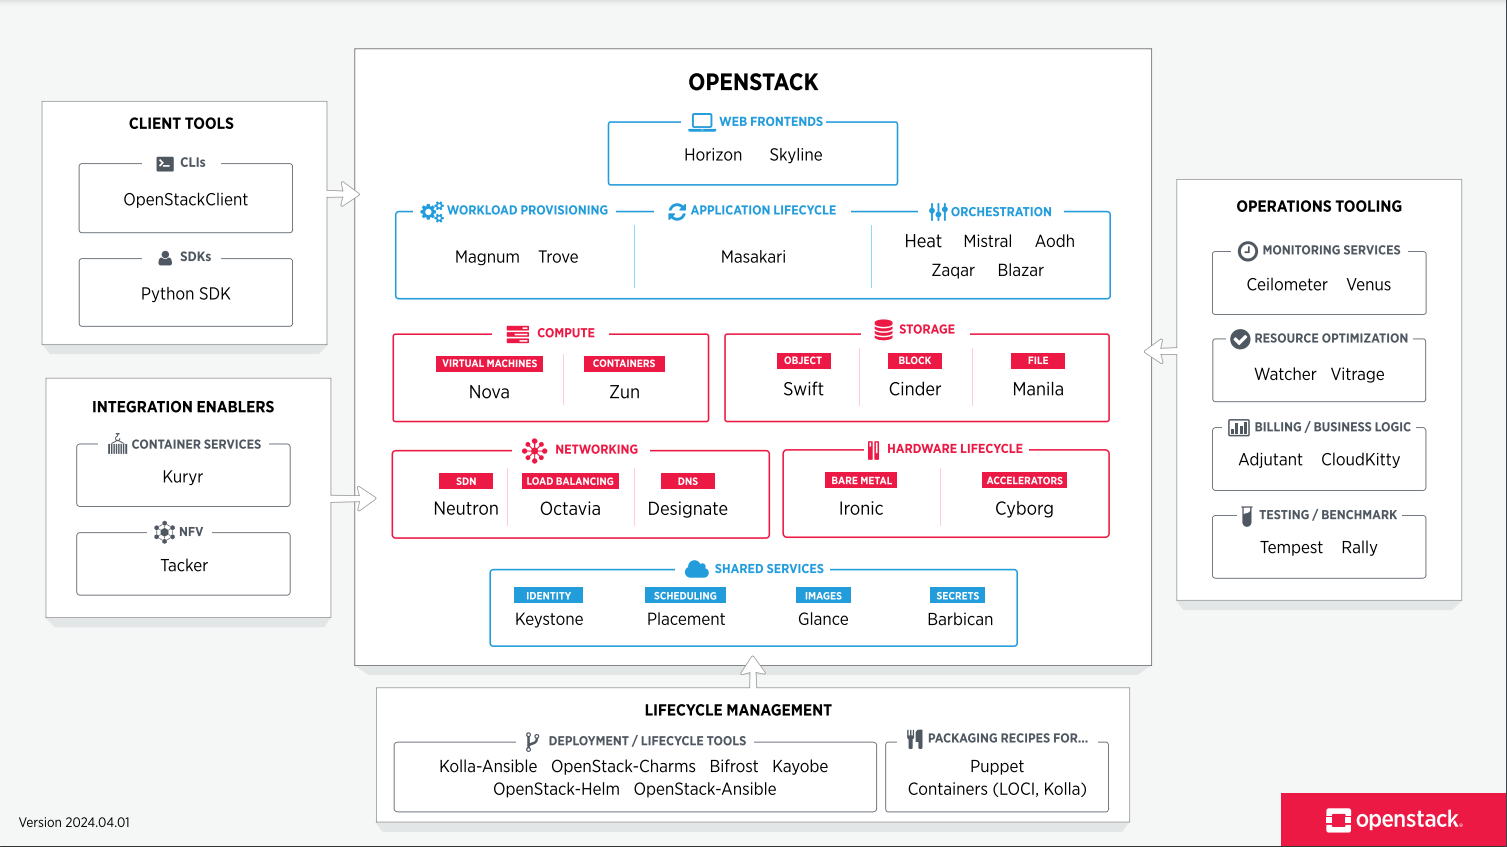
\includegraphics[width=0.8\textwidth]{images/map_openstack.png}
    \caption*{\textit{Fonte:} \url{https://www.openstack.org/software}.}
    \label{fig:map_openstack}
\end{figure}


\subsection{Principais Componentes}

A arquitetura do OpenStack, como comentado, é composta por vários componentes interconectados, cada um desempenhando uma função específica dentro do ambiente de nuvem. A Figura \ref{fig:openstack_conceptual_architecture} mostra a arquitetura conceitual do OpenStack, destacando como esses componentes colaboram para fornecer uma solução integrada e escalável. A seguir, são descritos os principais componentes do OpenStack:

\begin{itemize}
    \item \textbf{Nova (Compute): } Responsável pela criação e gerenciamento de instâncias de máquinas virtuais (VMs) e contêineres. Similar ao EC2 da AWS, o Nova oferece um serviço robusto para provisionamento de instâncias, integrando-se com outros componentes como Neutron e Cinder para garantir escalabilidade e eficiência (\cite{OpenStackNovaArchitecture}).
    \item \textbf{Neutron (Networking): } O Neutron é o serviço de rede do OpenStack, fornecendo conectividade como um serviço. Ele gerencia redes, sub-redes, roteadores, balanceadores de carga e firewalls, permitindo a criação e configuração de redes virtuais que conectam as instâncias gerenciadas pelo Nova (\cite{OpenStackNeutronArchitecture}).
    \item \textbf{Keystone (Identity Service): } O Keystone é o serviço de identidade e autenticação do OpenStack. Ele gerencia usuários e permissões, fornecendo uma estrutura centralizada de autenticação para todos os serviços do OpenStack e auxiliando na aplicação de políticas de acesso.
    \item \textbf{Cinder (Block Storage): } O Cinder gerencia volumes de armazenamento persistente, que podem ser anexados e desanexados de instâncias conforme necessário. Esses volumes são ideais para armazenamento de dados que requerem acesso rápido e alta durabilidade.
    \item \textbf{Swift (Object Storage): } O Swift é o sistema de armazenamento de objetos, projetado para armazenar e recuperar grandes quantidades de dados não estruturados. Ele armazena dados em contêineres distribuídos, oferecendo uma solução escalável e resiliente, ideal para arquivos estáticos, backups e outros dados que não requerem acesso frequente, funciona muito parecio ao \textit{S3} da AWS.
    \item \textbf{Glance (Image Service): } O Glance gerencia as imagens de disco usadas para inicializar instâncias. Ele permite o upload, armazenamento e recuperação de imagens diretamente pelo Horizon ou por APIs, suportando diversos formatos de imagem.
    \item \textbf{Horizon (Dashboard): } Horizon é a interface gráfica baseada na web do OpenStack. Ela permite aos usuários e administradores gerenciar todos os serviços disponíveis de maneira intuitiva, incluindo a criação de instâncias, configuração de redes e monitoramento de recursos.
    \item \textbf{Heat (Orchestration): } Heat é o serviço de orquestração que automatiza o provisionamento e gerenciamento de infraestrutura usando templates YAML. Com Heat, é possível definir pilhas de recursos e automatizar sua criação e configuração, facilitando a implementação de Infraestrutura como Código (IaC), também aceita implementações com Terraform.
    \item \textbf{Trove (Database as a Service): } O Trove fornece serviços de banco de dados gerenciados dentro do OpenStack. Ele permite a criação, manutenção e escalabilidade de bancos de dados, oferecendo uma solução flexível e fácil de usar para gerenciamento de dados, como o \textit{RDS (Relation Database Service)} da AWS.
\end{itemize}


\begin{figure}[htbp]
  \centering
  \caption{Arquitetura conceitual do OpenStack. A figura apresenta os principais componentes do OpenStack e suas respectivas funções, como \textit{Nova} para computação, \textit{Neutron} para redes e \textit{Cinder} para armazenamento em blocos, ilustrando a interação desses serviços em uma solução de nuvem integrada.}
  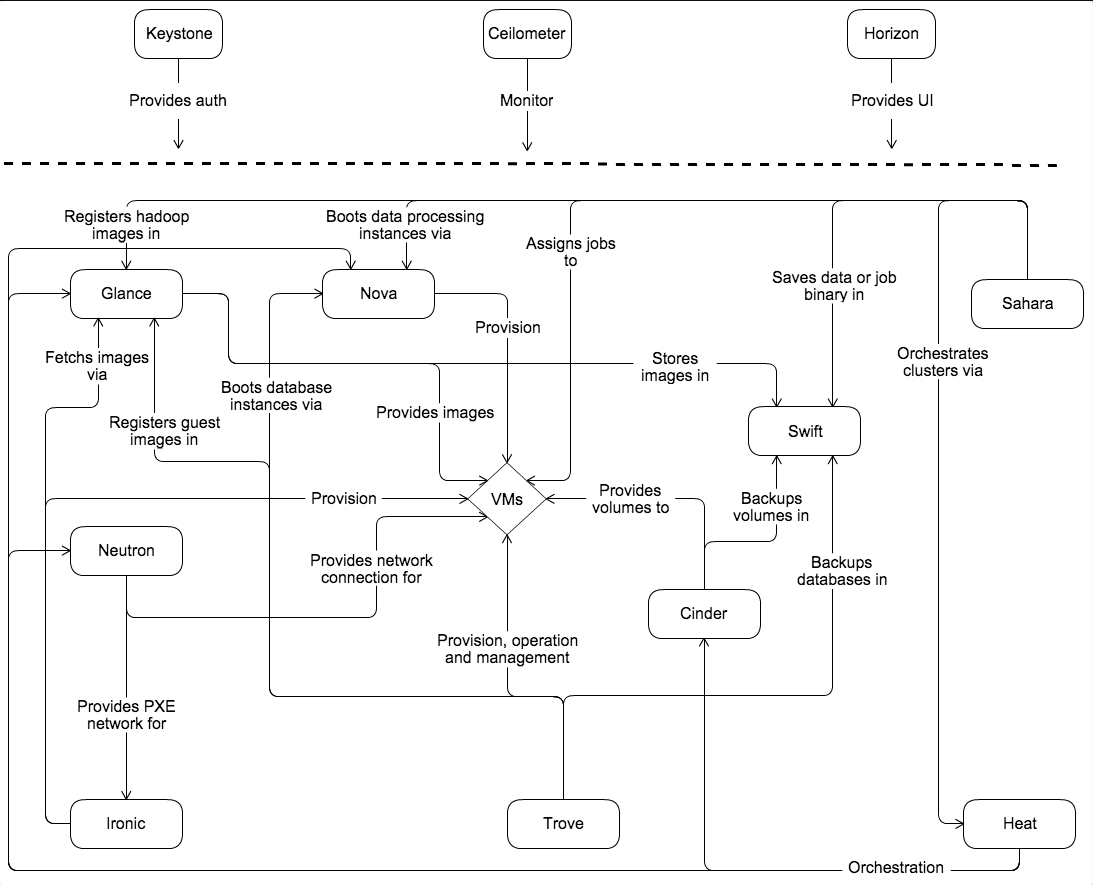
\includegraphics[width=0.8\textwidth]{images/architecture_conceptual_openstack.png}
  \caption*{\textit{Fonte:} \url{https://docs.openstack.org/install-guide/_images/openstack_kilo_conceptual_arch.png}.}
  \label{fig:openstack_conceptual_architecture}
\end{figure}


\section{Componentes do OpenStack}

Discutiremos em mais detalhes como funcionam internamente cada serviços mencionado anteriormente, mostrando como ele interage com o OpenStack de forma geral e suas principais responsabilidades. Focaremos neles porque eles serão essenciais na aplicação para a criação de um cluster.


\subsection{Nova (Compute)}

O \textbf{Nova} é o serviço de computação do OpenStack, responsável por gerenciar o ciclo de vida das instâncias de máquinas virtuais (VMs) e contêineres. Atuando como o motor de computação na nuvem, ele permite que os usuários provisionem e escalem recursos de maneira eficiente. Para provisionar uma instância funcional e acessível, o Nova interage com outros serviços do OpenStack, como Glance, Neutron, Keystone e Placement.

As principais funcionalidades do Nova incluem:

\begin{itemize}
    \item \textbf{Provisionamento de Instâncias:} Criação de instâncias de VMs com diferentes configurações de CPU, memória e armazenamento, atendendo a diversas necessidades de computação.
    \item \textbf{Suporte a Contêineres:} Execução de contêineres, proporcionando uma camada adicional de flexibilidade e eficiência.
    \item \textbf{Escalabilidade:} Administração de grandes quantidades de instâncias, distribuídas em diversos hosts e regiões, com alta escalabilidade.
    \item \textbf{Integração com Outros Componentes:} Interação transparente com serviços como Neutron para gerenciamento de rede e Cinder para armazenamento em blocos, garantindo alocação coordenada e eficiente dos recursos.
\end{itemize}

\subsection{Arquitetura do Nova}

A arquitetura do Nova é composta por vários subcomponentes que colaboram para gerenciar o ciclo de vida das instâncias (\cite{OpenStackNovaArchitecture}). Os principais subcomponentes incluem:

\begin{itemize}
    \item \textbf{nova-api:} Recebe as requisições dos usuários (via API ou Dashboard) e encaminha-as para os demais subcomponentes.
    \item \textbf{nova-scheduler:} Decide em qual nó de computação a instância será criada, consultando o serviço Placement para verificar a disponibilidade de recursos.
    \item \textbf{nova-conductor:} Atua como intermediário entre o nova-compute e o banco de dados, ajudando a minimizar a carga nos nós de computação.
    \item \textbf{nova-compute:} Gerencia a criação, modificação e destruição das instâncias em um nó de computação, interagindo com o hypervisor para executar as operações necessárias.
    \item \textbf{nova-placement:} Mantém informações sobre os recursos disponíveis e utilizados no cluster, auxiliando o nova-scheduler na tomada de decisões.
\end{itemize}


\begin{figure}[htbp]
  \centering
  \caption{Estrutura do Nova. A figura mostra os principais subcomponentes do serviço Nova, incluindo \textit{nova-api}, \textit{nova-scheduler}, \textit{nova-conductor}, \textit{nova-compute} e \textit{nova-placement}, e como eles interagem para gerenciar o ciclo de vida das instâncias.}
  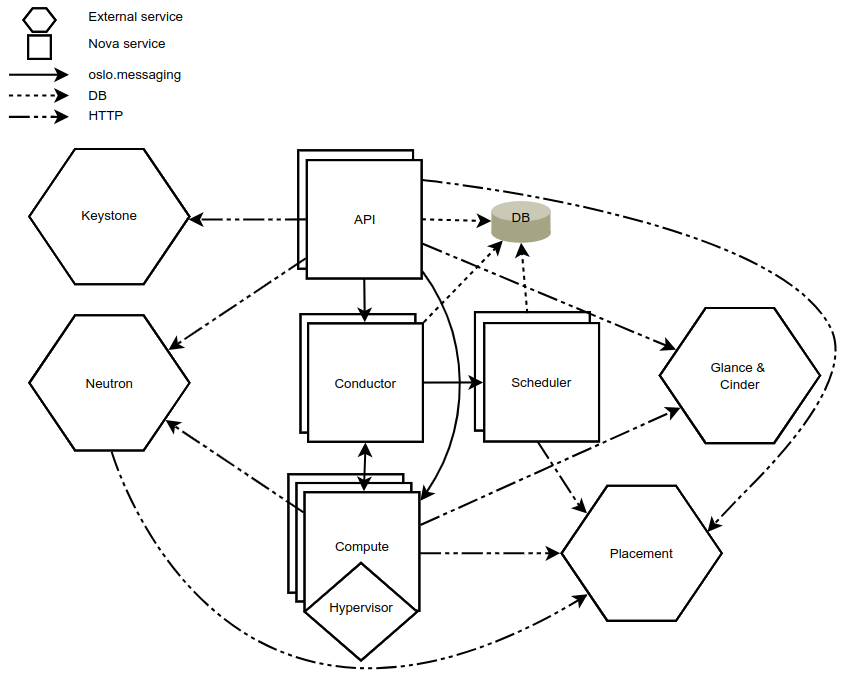
\includegraphics[width=0.7\textwidth]{images/nova_structure.png}
  \caption*{\textit{Fonte:} (\cite{DocumentacaoOpenstack}).}
  \label{fig:nova_structure}
\end{figure}


O processo de criação de uma instância no Nova segue estas etapas:

\begin{enumerate}
    \item \textbf{Recepção da Requisição:} O usuário envia uma solicitação para criar uma nova instância através da API do OpenStack.
    \item \textbf{Processamento Inicial:} O \textbf{nova-api} recebe a requisição, cria uma entrada no banco de dados e a coloca em uma fila para processamento pelo \textbf{nova-scheduler} (utilizando o RabbitMQ, um serviço popular de mensageria).
    \item \textbf{Escolha do Nó de Computação:} O \textbf{nova-scheduler} lê a requisição da fila, consulta o \textbf{nova-placement} para verificar a disponibilidade de recursos e seleciona o nó mais adequado aplicando filtros e políticas.
    \item \textbf{Intermediação do Conductor:} O \textbf{nova-conductor} envia as instruções necessárias ao \textbf{nova-compute} do nó selecionado.
    \item \textbf{Interação com o Hypervisor:} O \textbf{nova-compute} se comunica com o hypervisor (como QEMU-KVM) para criar a instância, configurando a rede via Neutron e anexando volumes de armazenamento via Cinder, se necessário.
    \item \textbf{Inicialização da Instância:} Após a criação, a instância é iniciada, e o \textbf{nova-compute} atualiza o estado da instância no banco de dados.
\end{enumerate}


Na escolha do nó de computação, o \textbf{nova-scheduler} aplica diversos filtros para garantir a alocação eficiente das instâncias. Alguns dos principais filtros incluem:

\begin{itemize}
    \item \textbf{AggregateIoOpsFilter:} Filtra nós com base na carga de operações de I/O.
    \item \textbf{AggregateNumInstancesFilter:} Limita o número de instâncias por nó.
    \item \textbf{ComputeCapabilitiesFilter:} Avalia as capacidades de computação dos nós.
    \item \textbf{RamFilter:} Verifica a quantidade de memória RAM disponível.
    \item \textbf{DiskFilter:} Considera a disponibilidade de espaço em disco.
\end{itemize}

Além da criação de instâncias, o Nova gerencia outras operações do ciclo de vida, como:

\begin{itemize}
    \item \textbf{Escalabilidade:} Permite a escala horizontal de instâncias, assegurando o crescimento da infraestrutura conforme necessário.
    \item \textbf{Migração:} Suporta a migração de instâncias entre nós de computação para manutenção ou balanceamento de carga.
    \item \textbf{Redimensionamento:} Permite o ajuste de recursos alocados a uma instância existente.
    \item \textbf{Monitoramento e Recuperação:} Monitora o estado das instâncias e realiza ações corretivas em caso de falhas.
\end{itemize}


\subsection{Neutron (Networking)}

O \textbf{Neutron} é o serviço de gerenciamento e criação de rede, responsável por fornecer conectividade como um serviço entre os componentes do ambiente de nuvem. Ele permite que os usuários criem e gerenciem redes virtuais, sub-redes, roteadores, balanceadores de carga, firewalls e outros recursos de rede de maneira programática, garantindo que as instâncias possam se comunicar entre si e com redes externas.

O Neutron oferece uma ampla gama de funcionalidades que permitem a configuração e gerenciamento de redes de forma flexível e escalável:

\begin{itemize}
    \item \textbf{Criação de Redes Virtuais:} Permite a criação de redes virtuais que conectam as instâncias de VMs, proporcionando isolamento entre diferentes grupos de usuários ou projetos.
    \item \textbf{Gerenciamento de Sub-redes:} Facilita a criação de sub-redes dentro das redes virtuais, com suporte para alocação automática de endereços IP (DHCP) e configuração de gateway.
    \item \textbf{Roteamento e NAT:} Suporta a configuração de roteadores para interconectar sub-redes e fornecer acesso externo às instâncias, incluindo suporte para NAT (Network Address Translation).
    \item \textbf{Segurança de Rede:} Inclui a configuração de firewalls e grupos de segurança que controlam o tráfego de entrada e saída da rede, garantindo um ambiente seguro.
    \item \textbf{Balanceamento de Carga:} Oferece serviços de balanceamento de carga para distribuir o tráfego entre múltiplas instâncias, melhorando a disponibilidade e o desempenho dos aplicativos.
\end{itemize}

Assim como o Nova a arquitetura do Neutron é composta por diversos componentes que colaboram para gerenciar a rede em um ambiente OpenStack. Os principais componentes incluem:

\begin{itemize}
    \item \textbf{neutron-server:} Componente central que expõe as APIs do Neutron e orquestra as operações de rede, interagindo com o banco de dados e os agentes de rede.
    \item \textbf{neutron-plugin:} Abstrai a interação com diferentes tecnologias de rede (como Open vSwitch, Linux Bridge, etc.), permitindo que o Neutron seja compatível com uma variedade de backends.
    \item \textbf{neutron-dhcp-agent:} Gerencia os serviços DHCP para as sub-redes, garantindo que as instâncias recebam endereços IP automaticamente.
    \item \textbf{neutron-l3-agent:} Responsável pelo roteamento de tráfego entre sub-redes e entre a rede interna e externa, implementando funcionalidades de roteamento e NAT.
    \item \textbf{neutron-metadata-agent:} Facilita o acesso das instâncias aos metadados necessários para sua configuração, como as chaves SSH ou dados de inicialização.
    \item \textbf{neutron-lbaas-agent:} Gerencia as operações de balanceamento de carga, criando e configurando balanceadores de carga conforme necessário.
\end{itemize}

\begin{figure}[htbp]
  \centering
  \caption{Fluxo de trabalho do Neutron. A figura ilustra os principais componentes do Neutron, como \textit{neutron-server}, agentes de DHCP, L3, metadados e balanceamento de carga, demonstrando como eles colaboram para fornecer serviços de rede em ambientes OpenStack.}
  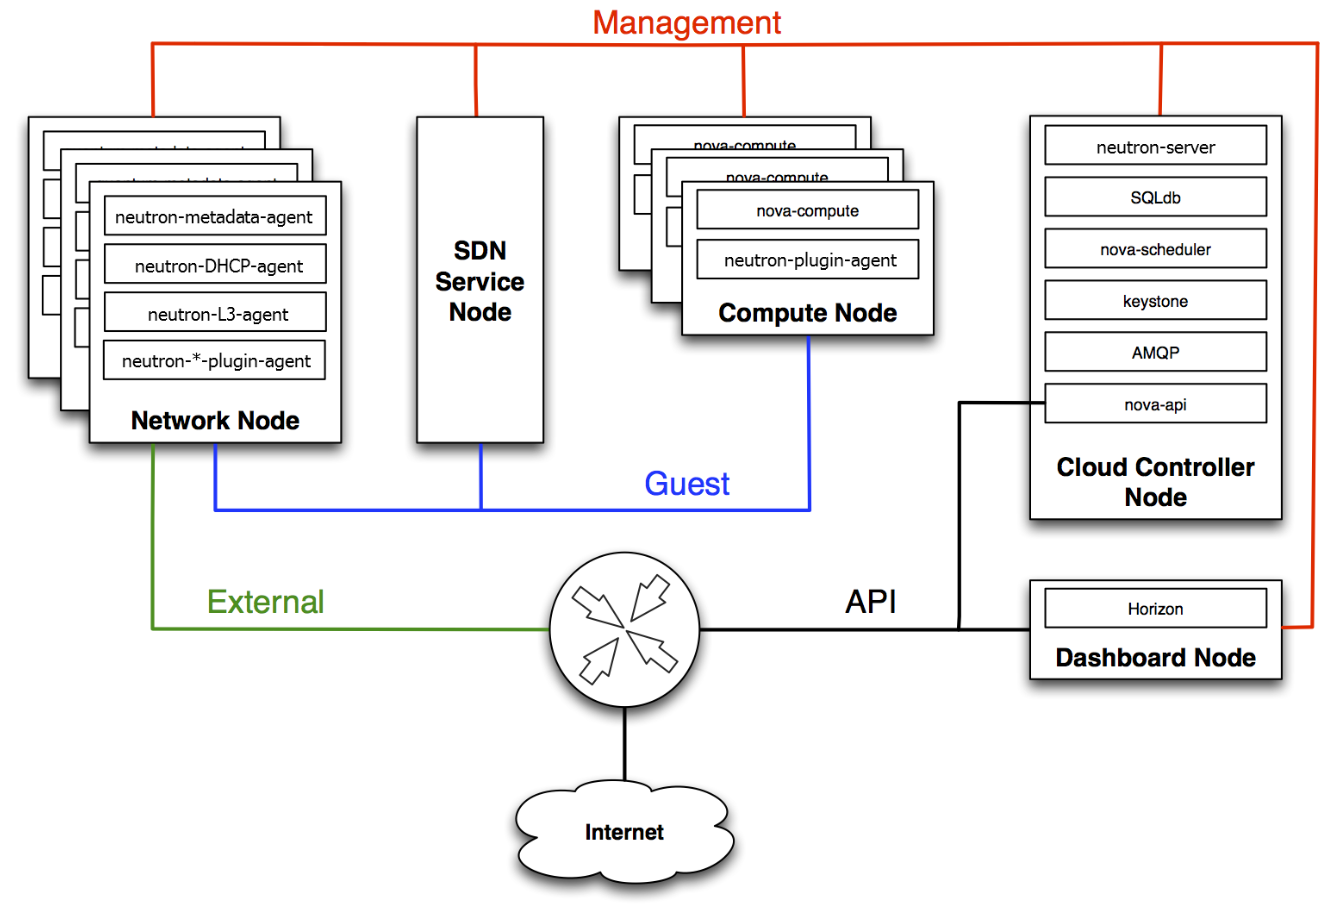
\includegraphics[width=0.8\textwidth]{images/architecture_neutron.png}
  \caption*{\textit{Fonte:} (\cite{DocumentacaoOpenstack}).}
  \label{fig:neutron_architecture}
\end{figure}


O processo de criação de uma rede e suas operações no Neutron envolvem várias etapas, que podem ser descritas da seguinte maneira:

\begin{enumerate}
    \item \textbf{Criação de Rede:} O usuário solicita a criação de uma rede virtual via API do Neutron, que é processada pelo \textbf{neutron-server}.
    \item \textbf{Configuração de Sub-rede:} O usuário define uma sub-rede dentro da rede criada, configurando parâmetros como o intervalo de endereços IP, gateway e servidor DHCP.
    \item \textbf{Configuração de Segurança:} O usuário configura grupos de segurança e regras de firewall para controlar o tráfego permitido a conexão para as instâncias conectadas à rede.
    \item \textbf{Roteamento e NAT:} Se necessário, o usuário cria um roteador para interligar sub-redes ou conectar a rede à internet, configurando NAT para que as instâncias possam acessar redes externas.
    \item \textbf{Balanceamento de Carga:} Para distribuir o tráfego entre várias instâncias, o usuário pode configurar um serviço de balanceamento de carga, que será gerenciado pelo \textbf{neutron-lbaas-agent}. Não é necessário criar diretamente um balanceador de carga
\end{enumerate}

A maneira como ela vai ser configurada dentro do OpenStack vai depender totalmente da necessidade do projeto.

\subsection{Keystone (Identity Service)}

O \textbf{Keystone} é o serviço de identidade do OpenStack, responsável por autenticar e autorizar usuários e serviços que interagem dentro da nuvem. Ele desempenha um papel central na segurança e no gerenciamento de acesso, garantindo que apenas usuários e serviços autenticados possam acessar os recursos disponíveis no OpenStack.


O Keystone oferece várias funcionalidades essenciais para a verficação de identidade e controle de acesso:

\begin{itemize}
    \item \textbf{Autenticação e Autorização:} O Keystone valida as credenciais dos usuários e serviços, emitindo tokens que são utilizados para autorizar o acesso aos outros componentes do OpenStack. Esses tokens carregam informações sobre as permissões do usuário ou serviço, garantindo que eles possam acessar apenas os recursos para os quais têm permissão.
    \item \textbf{Gerenciamento de Identidades:} O Keystone gerencia os usuários, grupos, projetos e domínios dentro do OpenStack. Ele permite a criação e atribuição de papéis \textit{(Roles)}, que determinam o nível de acesso e as permissões que cada usuário ou serviço tem dentro de um projeto ou domínio específico.
    \item \textbf{Serviço de Catálogo:} O Keystone mantém um catálogo dos serviços disponíveis no OpenStack, dentro do Horizon podemos ver as respectivas APIs e endpoints. Isso permite que os usuários e serviços descubram e interajam com outros componentes de maneira centralizada e eficiente.
\end{itemize}


O Keystone funciona como uma camada de segurança intermediária que se integra com todos os outros serviços do OpenStack. Quando um usuário ou serviço precisa acessar um recurso, ele primeiro se autentica no Keystone, que verifica as credenciais fornecidas (por exemplo, nome de usuário e senha, ou token). Se a autenticação for bem-sucedida, o Keystone emite um token que o usuário ou serviço pode usar para acessar outros componentes, como Nova, Neutron, ou Glance.

Cada vez que uma solicitação é feita a um serviço do OpenStack, o token é enviado como parte da requisição. O serviço verifica o token com o Keystone para garantir que ele seja válido e que o usuário ou serviço tenha as permissões necessárias para realizar a operação solicitada. Se o token for válido e as permissões forem adequadas, o serviço processa a requisição.

\subsection{Interação KeyStone com outros componentes}
O Keystone é essencial para a operação segura e eficiente de toda a infraestrutura do OpenStack. Todos os serviços, como Nova, Neutron, Glance, Cinder, e Swift, dependem do Keystone para autenticação e autorização. Quando um serviço precisa verificar as permissões de um usuário, ele consulta o Keystone, o que garante que todas as operações dentro do OpenStack estejam protegidas por um controle de acesso robusto (\cite{da2018self}).

\begin{figure}[htbp]
  \centering
  \caption{Autenticação de serviços e usuários no Keystone. A figura demonstra como o Keystone gerencia a autenticação e autorização de usuários e serviços no OpenStack, emitindo tokens e verificando permissões para garantir acesso seguro aos recursos.}
  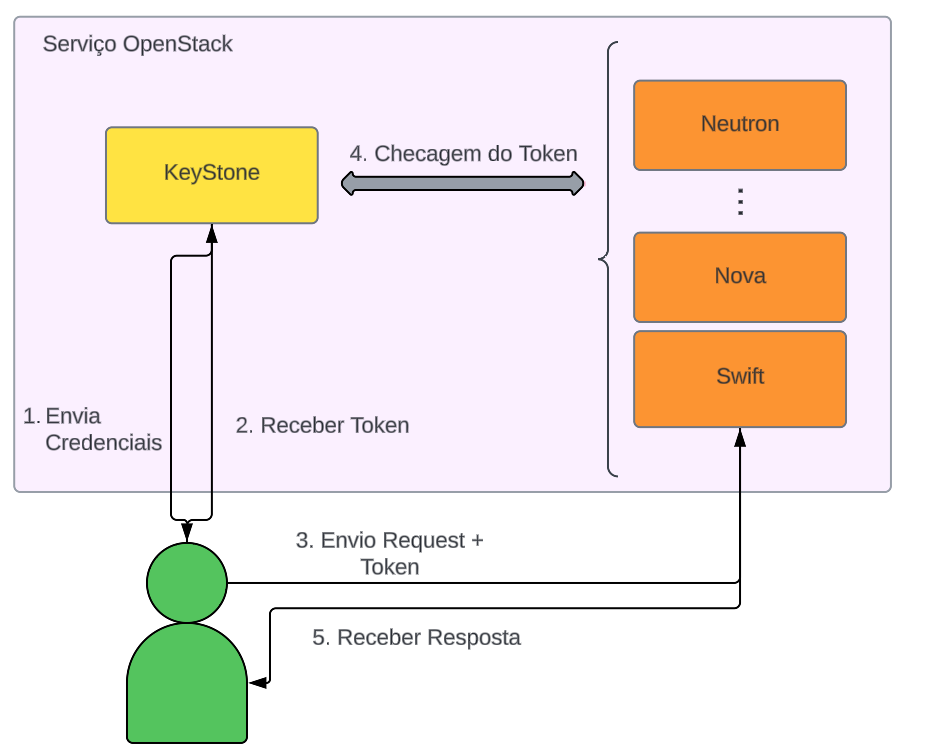
\includegraphics[width=0.7\textwidth]{images/keystone_architecture_2.png}
  \caption*{\textit{Fonte:} Adaptado de (\cite{da2018self}).}
  \label{fig:keystone_architecture}
\end{figure}


Além disso, o catálogo de serviços mantido pelo Keystone é fundamental para que os usuários e serviços descubram quais APIs e endpoints estão disponíveis, facilitando a comunicação e interação dentro do ambiente de nuvem.

Por fim, a capacidade do Keystone de integrar-se com sistemas de autenticação externos, através de federação e SSO, torna-o altamente versátil e adaptável a diferentes ambientes corporativos, garantindo uma experiência de usuário coesa e segura em organizações de todos os tamanhos.

Este papel central do Keystone na segurança e no gerenciamento de acesso faz dele um componente crítico no ecossistema OpenStack, assegurando que apenas usuários e serviços autorizados possam operar dentro da nuvem.


\subsection{Cinder (Block Storage)}

O \textbf{Cinder} é o serviço de armazenamento em bloco, responsável por gerenciar volumes de armazenamento que podem ser anexados a instâncias de máquinas virtuais. Ele fornece uma solução flexível e escalável para armazenar dados de maneira persistente, permitindo que os volumes sejam criados, gerenciados e conectados ou desconectados de instâncias conforme necessário (\cite{rosado2014overview}).

O armazenamento em bloco divide os dados em blocos e os armazena em partes separadas cada um com identificador exclusivo, dentro do sistema cada bloco é tratado como um disco individual, utilizamos dele para dar armazenamento a instância. Essa forma deixa fácil a duplicação do armazenamento para copias ou recuperar dados (\cite{BlockStorage}).

As principais funcionalidades do Cinder incluem:

\begin{itemize}
    \item \textbf{Criação e Gerenciamento de Volumes:} Permite que os usuários criem volumes de armazenamento que podem ser anexados a instâncias para uso como discos adicionais. Esses volumes podem ser criados a partir de imagens, snapshots, ou de forma vazia.
    \item \textbf{Snapshots:} O Cinder suporta a criação de snapshots de volumes, permitindo que os dados sejam salvos em um ponto no tempo para backup ou clonagem futura.
    \item \textbf{Tipos de Armazenamento:} Oferece a possibilidade de definir diferentes tipos de armazenamento, permitindo a escolha entre diversos backends de armazenamento com diferentes características de desempenho e custo.
    \item \textbf{Expansão de Volumes:} Volumes existentes podem ser expandidos conforme necessário, sem a necessidade de desconectar o volume da instância.
    \item \textbf{Conectividade Multi-backend:} Suporta múltiplos backends de armazenamento, como LVM, NFS, Ceph, e outros, proporcionando flexibilidade na escolha do hardware e arquitetura de armazenamento.
\end{itemize}

A arquitetura geral do Cinder se divide em:

\begin{itemize}
    \item \textbf{Cinder-API}: Exposição da interface RESTful para gerenciamento de volumes.
    \item \textbf{Cinder-Scheduler}: Responsável por determinar qual backend de armazenamento deve ser usado para criar um volume.
    \item \textbf{Cinder-Volume}: Gerenciamento direto de volumes nos backends de armazenamento.
    \item \textbf{Cinder-Backup}: Criação e gerenciamento de backups de volumes em armazenamento    secundário.
    \item \textbf{Cinder-Client}: Ferramenta de linha de comando para interagir com a API do Cinder.
\end{itemize}


\begin{figure}[htbp]
  \centering
  \caption{Arquitetura do Cinder. A figura apresenta os principais componentes do serviço Cinder, incluindo \textit{cinder-api}, \textit{cinder-scheduler}, \textit{cinder-volume}, \textit{cinder-backup}, e \textit{cinder-client}, ilustrando como eles colaboram para fornecer armazenamento em bloco persistente e escalável no OpenStack.}
  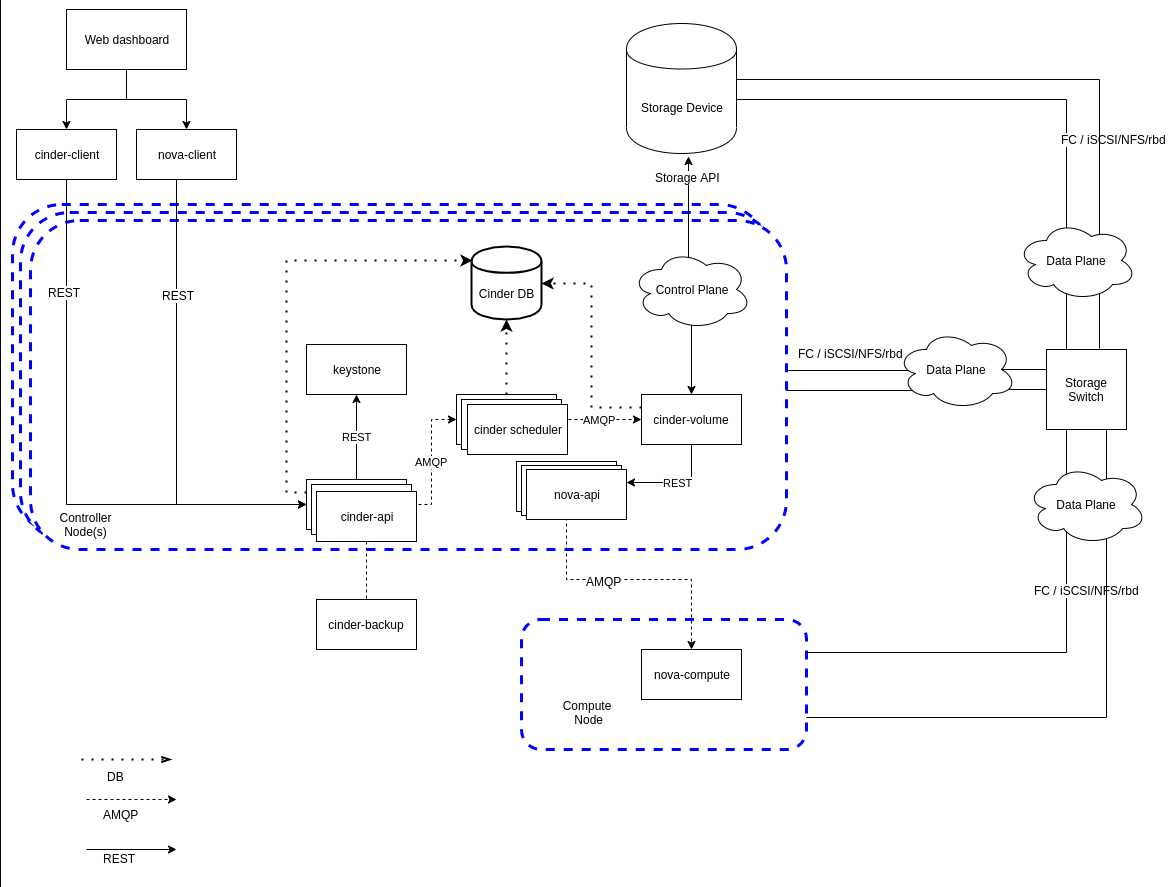
\includegraphics[width=0.95\textwidth]{images/cinder_architecture.png}
  \caption*{\textit{Fonte:} (\cite{OpenStackCinder}).}
  \label{fig:cinder_architecture}
\end{figure}


O Cinder é crucial para aplicações que exigem armazenamento de dados persistente e de alto desempenho, como bancos de dados e sistemas de arquivos distribuídos. Sua capacidade de integrar-se com diversos tipos de armazenamento e fornecer snapshots e backups automáticos torna-o um componente vital para a infraestrutura de nuvem do OpenStack por se ligar as instâncias (\cite{OpenStackCinder}).


\subsection{Swift (Object Storage)}

O \textbf{Swift} é o serviço de armazenamento de objetos, projetado para armazenar e recuperar grandes volumes de dados não estruturados de forma escalável e redundante. Diferente do armazenamento em bloco, o Swift armazena dados como objetos, que são agrupados em contêineres e acessados via uma API RESTful, sem a necessidade de gerenciar um sistema de arquivos tradicional (\cite{OpenStackSwitft}), segue a mesma ideia do \textit{S3 AWS}, assim você consegue salvar todos os arquivos e acessar eles pelo ID de forma eficiênte via API.

O armazenamento de objetos encapsula dados em unidades chamadas objetos, que incluem tanto os dados quanto seus metadados e atributos. Essa abordagem permite um gerenciamento mais flexível e escalável dos dados, distribuindo a carga de trabalho entre dispositivos de armazenamento inteligentes, conhecidos como Object-based Storage Devices (OSDs), que oferecem alta performance e segurança em ambientes de computação distribuída" (\cite{panasas2007object}).

As principais funcionalidades do Swift incluem:

\begin{itemize}
    \item \textbf{Armazenamento Escalável de Objetos:} Permite armazenar uma quantidade ilimitada de dados distribuídos entre múltiplos servidores, garantindo escalabilidade horizontal.
    \item \textbf{Redundância e Replicação:} Implementa replicação automática dos dados para assegurar alta disponibilidade e durabilidade, mesmo em caso de falhas de hardware.
    \item \textbf{Acesso via API RESTful:} Os dados podem ser acessados e gerenciados através de uma API RESTful, facilitando a integração com aplicações e serviços web.
    \item \textbf{Gerenciamento de Contêineres:} Organiza os objetos em contêineres, permitindo que os usuários agrupem dados logicamente e definam políticas de acesso específicas.
    \item \textbf{Versionamento e Auditoria:} Suporta versionamento de objetos e auditoria de acessos, garantindo controle sobre as mudanças e acesso aos dados.
\end{itemize}

O Swift é ideal para armazenar grandes quantidades de dados não estruturados, como backups, arquivos multimídia, e logs. Sua arquitetura distribuída e resiliente o torna uma escolha popular para ambientes que exigem armazenamento de longa duração e alta disponibilidade.

\subsection{Glance (Image Service)}

O \textbf{Glance} é o serviço de gerenciamento de imagens, projetado para armazenar, descobrir e recuperar imagens de disco de máquinas virtuais. Ele permite que os usuários façam upload de imagens de sistemas operacionais e outros discos, que podem ser usados para instanciar novas máquinas virtuais. As imagens podem ser armazenadas em uma variedade de backends, como Swift, Ceph, ou em sistemas de arquivos locais.

As principais funcionalidades do Glance incluem:

\begin{itemize}
    \item \textbf{Gerenciamento de Imagens:} Facilita o upload, armazenamento e compartilhamento de imagens de disco, que podem ser usadas para criar novas instâncias de VMs.
    \item \textbf{Conversão de Formatos:} Glance pode converter imagens entre diferentes formatos de disco, proporcionando maior compatibilidade e flexibilidade na utilização das imagens.
\end{itemize}

O Glance é essencial para o provisionamento de instâncias no OpenStack, permitindo que as imagens de sistemas operacionais e discos sejam gerenciadas de forma centralizada e eficiente. Sua integração com outros componentes do OpenStack, como Nova e Cinder, torna-o um elemento crucial para a operação e escalabilidade da nuvem.

\subsection{Heat (Infraestructure as a Code)}

O \textbf{Heat} é o serviço de orquestração de recursos, projetado para permitir o gerenciamento automatizado e coordenado de infraestruturas complexas. Utilizando templates escritos em YAML, o Heat facilita a criação e o gerenciamento de pilhas de recursos, como instâncias de computação, volumes de armazenamento, redes e outros serviços do OpenStack, de forma declarativa e repetível (\cite{OpenStackHeat}).

O Heat permite que orquestremos toda a infraestrutura de uma organização específica com templates, aceita também o Terraform e o CloudFormation, dois serviços famosos de IaaC, a ideia de utilizar esses templates é basicamente configurar um ambiente e não precisar ficar refazendo ele caso necessário, você tem todo controle no template e sabe exatamente quais passos foram feitos para construção ou alocação de determinado recurso.

As principais funcionalidades do Heat incluem:

\begin{itemize}
    \item \textbf{Orquestração de Pilhas de Recursos:} Gerencia a criação, atualização e exclusão de conjuntos de recursos interdependentes como uma única unidade, chamada de pilha (\textit{stack}).
    \item \textbf{Infraestrutura como Código:} Os usuários podem definir a infraestrutura em templates YAML, que descrevem os recursos e as relações entre eles, permitindo a automação de operações e a reprodutibilidade dos ambientes.
    \item \textbf{Automação de Provisionamento:} Suporta a automação de tarefas repetitivas e complexas, como o escalonamento de instâncias de computação e o provisionamento de redes e volumes.
    \item \textbf{Suporte a Vários Templates:} Além dos templates nativos do Heat (HOT - Heat Orchestration Template), também suporta templates no formato AWS CloudFormation, proporcionando flexibilidade na definição dos recursos.
\end{itemize}


\href{https://docs.openstack.org/heat/latest/developing_guides/architecture.html}{Arquitetura geral Heat}:

\begin{itemize}
    \item \textbf{Heat-engine:} É o componente central responsável pelo gerenciamento das pilhas de recursos (\textit{stacks}). O Heat Engine interpreta os templates, cria e gerencia os recursos descritos nos templates, e lida com as operações de ciclo de vida das pilhas, como criação, atualização e exclusão.
    \item \textbf{Heat-api:} Fornece uma interface RESTful que permite aos usuários interagir com o serviço Heat. Através da Heat API, os usuários podem enviar templates, criar e gerenciar pilhas, e consultar o estado das pilhas e recursos.
    \item \textbf{Heat-api-cfn:} Implementa uma API compatível com AWS CloudFormation, permitindo que os usuários usem templates no formato AWS CloudFormation para definir e gerenciar seus recursos. Isso oferece uma compatibilidade adicional para aqueles que estão familiarizados com a infraestrutura como código.
    \item \textbf{Python-heatclient:} É a ferramenta de linha de comando que permite interagir com o serviço Heat. Os usuários podem usar o Heat Client para executar comandos que criam, atualizam, deletam e listam pilhas e recursos no OpenStack.
\end{itemize}


O Heat é ideal para automatizar a implementação e o gerenciamento de infraestruturas complexas e repetitivas em ambientes de nuvem, garantindo consistência, escalabilidade e eficiência operacionais. Sua capacidade de orquestrar diversos serviços do OpenStack em conjunto torna-o uma ferramenta essencial para DevOps e equipes de operações que buscam simplificar a gestão de infraestrutura na nuvem.


\subsection{Trove (Database as a Service)}

O \textbf{Trove} é o serviço de banco de dados como serviço (DBaaS) do OpenStack, projetado para simplificar o gerenciamento e a operação de bancos de dados relacionais e não relacionais em ambientes de nuvem. O Trove permite aos usuários provisionar, configurar, operar e escalar instâncias de banco de dados com facilidade, utilizando uma interface unificada e integrada ao ecossistema OpenStack (\cite{OpenStackTrove}).

O Trove possibilita o gerenciamento de múltiplos bancos de dados através de uma API RESTful, oferecendo suporte para diversos tipos de bancos de dados, como MySQL, PostgreSQL, MongoDB, entre outros. Isso permite que as organizações mantenham uma infraestrutura de banco de dados flexível e escalável, sem a complexidade tradicional associada à administração de bancos de dados em larga escala.

As principais funcionalidades do Trove incluem:

\begin{itemize}
    \item \textbf{Provisionamento Automatizado de Bancos de Dados:} Facilita a criação de instâncias de banco de dados de forma automatizada, permitindo o provisionamento rápido e eficiente de bancos de dados para diferentes aplicações.
    \item \textbf{Gestão Simplificada:} Oferece ferramentas para gerenciar facilmente backups, restaurações, atualizações de software e monitoramento de desempenho, simplificando a administração de bancos de dados.
    \item \textbf{Suporte a Múltiplos Motores de Banco de Dados:} O Trove suporta uma variedade de motores de banco de dados, tanto relacionais quanto não relacionais, proporcionando flexibilidade para diferentes necessidades de aplicação.
    \item \textbf{Escalabilidade:} Permite a escalabilidade vertical e horizontal das instâncias de banco de dados, garantindo que os recursos possam ser ajustados conforme a demanda aumenta.
\end{itemize}

\href{https://docs.openstack.org/trove/latest/contributor/design.html}{Arquitetura geral do Trove}:

\begin{itemize}
    \item \textbf{Trove-taskmanager:} Responsável por gerenciar as operações assíncronas no Trove, como a criação de instâncias, backups e restaurações. Ele coordena essas tarefas em segundo plano para garantir que sejam executadas de forma eficiente.
    \item \textbf{Trove-api:} Fornece a interface RESTful através da qual os usuários podem interagir com o serviço Trove. Através da Trove API, os usuários podem criar, configurar e gerenciar instâncias de banco de dados.
    \item \textbf{Trove-conductor:} Atua como um intermediário entre o Trove-taskmanager e o banco de dados de controle do OpenStack, garantindo a integridade e a sincronização dos dados de gerenciamento.
    \item \textbf{Trove-guestagent:} Instalado dentro de cada instância de banco de dados provisionada pelo Trove, o Trove-guestagent é responsável por executar as operações específicas do banco de dados, como backups, restaurações e mudanças de configuração, comunicando-se com o Trove-taskmanager para realizar essas tarefas.
    \item \textbf{Python-troveclient:} É a ferramenta de linha de comando que permite aos usuários interagir diretamente com o serviço Trove. O Trove Client permite a execução de comandos para criar, gerenciar e excluir instâncias de banco de dados.
\end{itemize}

O Trove é ideal para organizações que desejam simplificar o gerenciamento de bancos de dados na nuvem, permitindo uma administração eficiente e escalável. Com o Trove, as equipes de operações podem automatizar o provisionamento e a manutenção de bancos de dados, garantindo um desempenho consistente e reduzindo a complexidade operacional.


\subsection{Recapitulando}

Como vimos, o OpenStack é composto por diversos componentes que interagem entre si para formar uma infraestrutura como serviço (IaaS) robusta e escalável. Exploramos em detalhe alguns dos componentes mais importantes, como Nova, Neutron e Keystone, que são fundamentais para o funcionamento do OpenStack e serão amplamente utilizados na implementação do nosso projeto.

O OpenStack continua a evoluir, ganhando popularidade e recebendo novas funcionalidades a cada ano. Por essa razão, a análise dos componentes foi abordada de forma geral, destacando aspectos arquiteturais e operacionais essenciais. É importante ressaltar que, embora tenhamos focado nos componentes mais amplamente utilizados, o OpenStack oferece uma gama ainda maior de serviços que podem ser personalizados para atender a necessidades específicas.


\section{Orquestração de VMs}

A orquestração de VMs torna-se essencial em ambientes onde a quantidade de instâncias supera a capacidade de gerenciamento manual. Inicialmente, quando lidamos com poucas instâncias, o uso de um hypervisor para controlar as máquinas virtuais pode ser suficiente. Um Virtual Machine Monitor (VMM) pode monitorar logs, verificar o uso de recursos e reiniciar instâncias quando necessário. Entretanto, à medida que a infraestrutura se expande, o gerenciamento de dezenas ou centenas de VMs se torna inviável sem uma camada de orquestração.

Aqui entra o OpenStack, que proporciona uma plataforma escalável e flexível para gerenciar grandes quantidades de recursos computacionais. Ele automatiza tarefas como a criação de novas instâncias, a distribuição de recursos entre elas, e a recuperação de falhas, tudo isso através de uma interface centralizada. Para ilustrar, enquanto uma pequena empresa poderia gerenciar manualmente poucas instâncias, uma grande organização com picos de demanda e infraestrutura complexa, como uma empresa de e-commerce de grande porte, exigiria orquestração automática para manter a continuidade do serviço em momentos de alta carga, como em eventos sazonais.

A orquestração de VMs não se resume apenas à criação e destruição de instâncias, mas envolve uma série de processos automatizados, como provisionamento, escalabilidade automática, e monitoramento contínuo. Esses processos garantem que a infraestrutura esteja sempre otimizada e pronta para atender às demandas crescentes, minimizando o tempo de inatividade e maximizando a eficiência dos recursos.

\section{Orquestração de Containers}

A orquestração de containers segue uma lógica semelhante à de VMs, porém com um nível de granularidade e agilidade muito maior. Containers são instâncias leves que compartilham o mesmo sistema operacional do host, o que permite que sejam inicializados rapidamente e consumam menos recursos em comparação com VMs completas. No entanto, com a proliferação de containers em um ambiente de produção, gerenciá-los manualmente também se torna inviável. É aí que entra o Kubernetes, uma das ferramentas mais utilizadas para orquestração de containers.

O Kubernetes permite gerenciar de forma eficiente centenas ou até milhares de containers, distribuindo a carga de trabalho entre diferentes nós e garantindo que os serviços continuem funcionando, mesmo que algum nó falhe. Ele utiliza um sistema baseado em declarações em um arquivo \textit{.yaml}, onde o administrador define o estado desejado da aplicação (quantidade de containers, recursos utilizados, etc.), e o Kubernetes se encarrega de garantir que esse estado seja mantido.

Além disso, o Kubernetes facilita o escalonamento de aplicações, monitorando o desempenho dos containers e adicionando ou removendo instâncias conforme necessário. Isso é particularmente útil em arquiteturas baseadas em microserviços, onde diferentes partes de uma aplicação podem ser escaladas de maneira independente, melhorando a eficiência e o uso de recursos (\cite{KubernetsDocumentation}).

\subsection{Estrutura do Kubernetes}

O Kubernetes é composto por vários componentes que, juntos, formam um sistema robusto de orquestração como podemos ver na figura \ref{fig:structure_kubernets}. Os principais elementos da arquitetura do Kubernetes incluem:


\begin{figure}[htbp]
  \centering
  \caption{Estrutura do Kubernetes. A figura apresenta os principais componentes do Kubernetes, como nós, pods, plano de controle (\textit{Control Plane}), \textit{Scheduler}, \textit{Kubelet} e serviços, ilustrando como eles interagem para orquestrar aplicações distribuídas de forma eficiente.}
  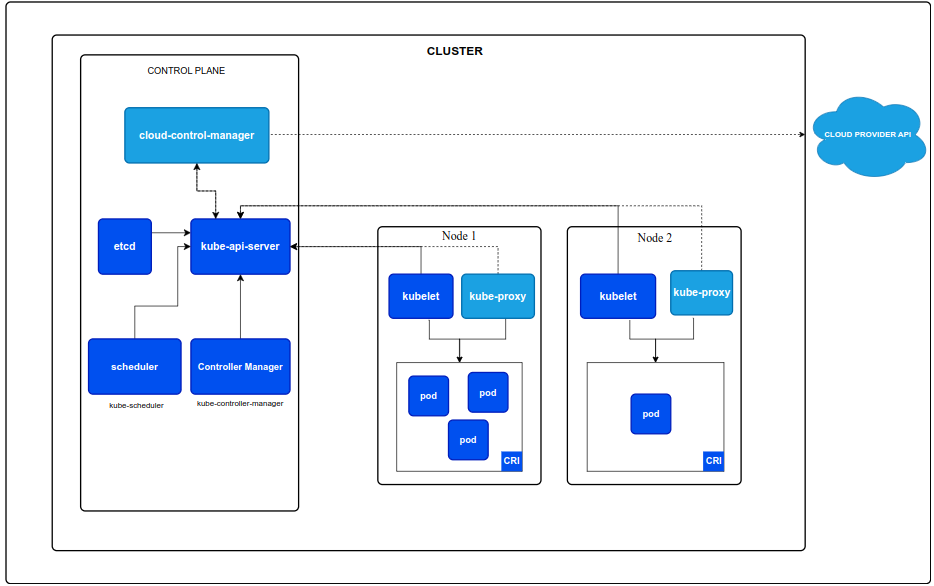
\includegraphics[width=0.9\textwidth]{images/structure_kubernets.png}
  \caption*{\textit{Fonte:} \url{https://kubernetes.io/docs/concepts/architecture/}.}
  \label{fig:structure_kubernets}
\end{figure}


\begin{itemize}
    \item \textbf{Nó (Node):} Cada máquina física ou virtual dentro do cluster do Kubernetes é chamada de nó. Um nó pode conter um ou mais containers.
    \item \textbf{Pods:} O pod é a menor unidade de execução no Kubernetes e pode conter um ou mais containers. Todos os containers dentro de um pod compartilham o mesmo endereço IP e espaço de rede, por padrão cada pod possui apenas um container.
    \item \textbf{Control Plane:} A camada de controle central que gerencia os nós do cluster e garante que o estado desejado das aplicações seja mantido.
    \item \textbf{Scheduler:} Responsável por alocar pods nos nós disponíveis de acordo com os requisitos de recursos e políticas definidas.
    \item \textbf{Kubelet:} Um agente que roda em cada nó do cluster e garante que os containers estejam executando conforme o especificado pelo Kubernetes.
    \item \textbf{Service:} Um serviço que expõe um conjunto de pods como uma única entidade, facilitando o balanceamento de carga e a descoberta de serviços.
\end{itemize}

Com essa arquitetura, o Kubernetes permite que as empresas implementem e gerenciem aplicações distribuídas de forma eficiente, garantindo alta disponibilidade, resiliência e facilidade de manutenção. Também pode ser feita a integração a nossa nuvem privada utilizando o componente Magnum do OpenStack.


  % \chapter{Metodologia}

A implementação de uma nuvem privada no Instituto Federal de Brasília (IFB) no campus de Taguatinga será conduzida de forma estruturada, abrangendo desde o planejamento inicial da infraestrutura até a implementação técnica e os testes necessários para assegurar o bom funcionamento da solução. A metodologia será dividida em quatro grandes etapas: planejamento da infraestrutura, configuração e implementação técnica, testes de infraestrutura e incentivo ao uso da nuvem privada.

\section{Etapa 1: Planejamento da Infraestrutura}

O primeiro passo para a criação da nuvem privada será a separação de um subconjunto de máquinas do Datacenter já existente no campus de Taguatinga. Será realizado um levantamento de máquinas ociosas e a separação de outras mais potentes, visando testar a escalabilidade do OpenStack como uma solução de nuvem privada. O hardware será reaproveitado para garantir a viabilidade econômica do projeto, e a escolha dos serviços a serem implementados no OpenStack será baseada nas necessidades acadêmicas e administrativas.

Nesta etapa, o planejamento incluirá a identificação dos servidores, processadores, memória RAM, armazenamento e dispositivos de rede no Datacenter do campus, priorizando o uso de máquinas ociosas e hardware remanescente. Em seguida, será realizada a definição dos principais serviços do OpenStack que serão utilizados, como Nova para gerenciamento de instâncias, Neutron para gerenciamento de rede e Swift para armazenamento, de acordo com as necessidades de escalabilidade e gerenciamento da nuvem privada. Finalmente, será feita uma avaliação da capacidade do hardware e da rede do campus para suportar a instalação do OpenStack e a orquestração dos serviços em um ambiente de nuvem privada.

\section{Etapa 2: Configuração e Implementação Técnica}

Após o planejamento da infraestrutura, será iniciada a instalação do OpenStack, configurando cada serviço em suas respectivas máquinas. Existem duas abordagens principais para instalar o OpenStack: via DevStack, voltada para desenvolvedores, ou por meio de um gerenciador de pacotes. Para este projeto, será escolhida a abordagem mais adequada às necessidades do campus, garantindo controle e facilidade de manutenção.

De forma geral a instalação via DevStack garante um ambiente flexível, configurando cada serviço em máquinas específicas e ajustando o \textit{local.conf} de cada máquina para operar em um cluster. A configuração dos serviços será distribuída de forma a garantir o balanceamento de carga, e o Kubernetes poderá ser utilizado em conjunto com o Docker para orquestrar contêineres, aumentando a eficiência da solução. Após a configuração, serão realizados testes básicos de conectividade entre os nós do cluster para garantir que os serviços estão comunicando corretamente e que a nuvem privada está pronta para os próximos passos.

\section{Etapa 3: Testes de Infraestrutura}

Testes de desempenho e saúde da infraestrutura serão realizados para garantir que o cluster da nuvem privada está funcionando corretamente e que a capacidade de expansão da solução está assegurada.

Os testes incluirão a simulação de diferentes níveis de utilização dos recursos, como memória, CPU e rede, para garantir que a infraestrutura pode suportar o uso interno, especialmente durante os períodos de maior demanda acadêmica, tentaremos entender qual vai ser a real necessidade com campus. Além disso, será realizada uma avaliação contínua da saúde do cluster, incluindo a verificação de latência, falhas de comunicação entre nós e monitoramento de uso de recursos para assegurar que a nuvem privada está operando de maneira eficiente. Também serão realizados testes de backup e recuperação de desastres para garantir que os dados e serviços possam ser restaurados rapidamente em caso de falhas.

\section{Etapa 4: Incentivo ao Uso da Nuvem Privada}

Após a implementação técnica e os testes, iniciara o incentivando o uso da nuvem privada em atividades acadêmicas.

As ações a serem realizadas incluem a integração da infraestrutura de nuvem privada dentro das disciplinas, permitindo que os alunos utilizem os recursos de nuvem em atividades práticas e trabalhos. Além disso, queremos que seja promovido o uso da nuvem privada em pesquisas científicas, disponibilizando recursos para que alunos e professores desenvolvam projetos de inovação utilizando a infraestrutura do campus.

Além disso, serão criados exemplos e aplicações práticas para serem utilizadas nas disciplinas do campus, como ambientes de desenvolvimento para projetos dos alunos, laboratórios virtuais e aplicações simples. Queremos que tenha uma interface web fácil de ser utilizado tanto pelos alunos como pelos professores, assegurando que a nuvem seja de fácil uso para todos os membros da comunidade acadêmica.

\section{Monitoramento e Avaliação Contínua}

Finalmente, será implementado um sistema de monitoramento contínuo da nuvem privada, com foco na manutenção da eficiência e na realização de ajustes conforme a demanda evolui.

As ações incluirão o acompanhamento em tempo real do uso de CPU, memória, disco e rede, com alertas em caso de sobrecarga ou falhas. Também será realizada a coleta de feedback regular dos usuários da nuvem para identificar problemas, sugestões de melhorias e novas necessidades. A partir desse feedback, serão realizados ajustes na configuração da infraestrutura e expansão do cluster conforme necessário, garantindo que a solução seja capaz de escalar conforme o aumento da demanda.

  % \chapter{Cronograma}

\section{Cronograma TCC}

\begin{flushright}
\begin{table}[h!]
        \begin{tabular}{|m{3cm}|c|c|c|c|c|c|}
        \hline
        \textbf{Atividade} & \textbf{Setembro} & \textbf{Outubro} & \textbf{Novembro} & \textbf{Dezembro} & \textbf{Janeiro} & \textbf{Fevereiro} \\ 
        \hline
        Fase de Planejamento &  & X &  &  &  &  \\
        \hline
        Desenvolvimento e Implementação &  & X & X &  &  &  \\
        \hline
        Testes de Integração &  &  & X & X &  &  \\
        \hline
        Escrita do TCC & X & X & X & X & X & X \\
        \hline
        \end{tabular}
        \label{tab:cronograma}
        \centering
        \caption{Cronograma de Atividades do TCC}
\end{table}
\end{flushright}

  
  \chapter{Projeto de Implementação do OpenStack no IFB}
\label{ref:implementation_project_openstack_ifb}

Todos os detalhes apresentados neste desenvolvimento foram baseados na documentação oficial do OpenStack~\citep{DocumentacaoOpenstack}. Algumas configurações específicas relacionadas às VMs foram obtidas em discussões sobre problemas registrados no \textit{\href{https://bugs.launchpad.net/openstack/}{lauchpad bugs (OpenStack)}}.

A finalidade deste capítulo é detalhar o processo de implementação do OpenStack no campus do Instituto Federal de Brasília, apresentando a arquitetura proposta, as configurações realizadas nos diferentes nós (Controller, Storage e Compute), e os ajustes necessários para atender às demandas específicas da instituição. Além disso, são abordadas estratégias de automação, criação de projetos para diferentes perfis de usuários e as considerações para futuras atualizações e migrações, garantindo a escalabilidade e a eficiência do ambiente implementado.


\section{Kolla}
Para construir nosso \textit{cluster} OpenStack, é necessário definir como o serviço será colocado em produção e como as máquinas serão distribuídas dentro do \textit{cluster}. Optamos pelo uso do \textit{\href{https://docs.openstack.org/kolla-ansible/latest/}{Kolla-Ansible}} devido à sua organização, facilidade de configuração e capacidade de automação.

O Kolla utiliza contêineres Docker para executar os serviços de forma isolada, proporcionando maior controle sobre cada componente. Essa abordagem permite escalar serviços, alterar imagens, adicionar configurações específicas e realizar modificações sem impactar os demais serviços do \textit{cluster}. A utilização de contêineres também facilita a manutenção e atualizações, uma vez que cada serviço opera de maneira independente.

Além disso, o Kolla-Ansible permite definir em qual nó cada serviço será executado, organizando grupos de controle que atribuem os contêineres aos nós correspondentes. Por padrão, o Nó principal (\textbf{Controller}) executa todos os serviços essenciais, enquanto os demais Nós recebem serviços específicos de acordo com suas funções, como \textit{Compute} ou \textit{Storage}. No entanto, também é possível configurar qualquer Nó para executar todos os serviços, dependendo da necessidade.

O OpenStack utiliza o \textbf{HAProxy} para realizar o balanceamento de carga entre os diferentes Nós, garantindo melhor distribuição do tráfego e alta disponibilidade. Isso elimina a necessidade de configurações adicionais de balanceamento, desde que os Nós estejam na mesma rede.

O Kolla oferece diferentes versões para organizar e gerenciar as imagens Docker de forma eficiente. No nosso caso, optamos pelo lançamento mais estável disponível no momento desta pesquisa, ``ubuntu-noble''. Essa escolha foi feita porque versões mais recentes nem sempre possuem todas as imagens \textit{builded}, o que pode levar à ausência de imagens importantes, como o \textit{Cinder} executando a versão ``rocky''. Para configurar a \textit{release} desejada, basta alterar a variável \texttt{openstack\_tag} no arquivo \texttt{globals.yaml} e executar o \textit{deploy}.

No Linux, o Python é essencial para o funcionamento de serviços do sistema, e alterar pacotes ou versões globalmente pode causar problemas. Por isso, é recomendável usar ambientes virtuais para isolar dependências de projetos, evitando interferências no sistema ou em outros projetos. Ferramentas como o pyenv permitem instalar e gerenciar versões específicas do Python de forma segura, criando ambientes virtuais dedicados sem afetar a versão padrão do sistema. Essa abordagem protege o sistema operacional e mantém um ambiente de desenvolvimento consistente. Para a instalação do kolla vamos utilizar o `python venv` e dentro dele instalar os pacotes essenciais do kolla como recomendado em \textit{\href{https://docs.openstack.org/kolla-ansible/latest/user/quickstart.html}{Kolla Ansible documentation}}.

Ao final do desenvolvimento, explicaremos como organizar nosso \textit{cluster} para facilitar futuras migrações e atualizações. Como os serviços estão isolados em contêineres, as atualizações tornam-se mais simples, permitindo a substituição individual de cada imagem sem impacto significativo nos demais serviços. Além disso, o Kolla garante uma retrocompatibilidade entre os contêineres, tornando a troca entre versões mais estável e segura.


\section{Hardware}

O objetivo principal é aproveitar o hardware remanescente para construir uma nuvem privada, com a possibilidade de, no futuro, expandir essa infraestrutura para uma nuvem completa. Essa expansão permitiria distribuir todo o hardware disponível de forma eficiente, beneficiando diretamente os alunos do campus. Além disso, será demonstrado adiante como essa abordagem simplifica a distribuição de poder computacional e oferece maior visibilidade sobre a utilização dos recursos em cada projeto.

Para a criação de um nó (Nó) simples do OpenStack, recomenda-se uma CPU com 24 núcleos, 24 GB ou mais de memória RAM e 4 discos de 500 GB (7200 RPM)~\citep{DocumentacaoOpenstack}, conforme ilustrado na Figura \ref{fig:hardware_requirements}. Como o cluster é composto por 3 nós, esses recursos precisariam ser triplicados para atender às demandas do ambiente.

Devido às limitações do hardware disponível, essa configuração não é viável. Portanto, será criado apenas para fins de demonstração e apresentaremos a arquitetura do cluster, como deveria ser feito em servidores em produção, a forma como vamos estrutura essa arquitetura deixa simples a adição e substituição de mais nós.

\begin{figure}[htbp]
    \centering
    \caption{Requisitos de hardware recomendados para a criação de um Nó OpenStack. A figura apresenta as especificações mínimas de CPU, memória e armazenamento necessárias para um nó OpenStack simples, com recomendações para ambientes de produção.}
    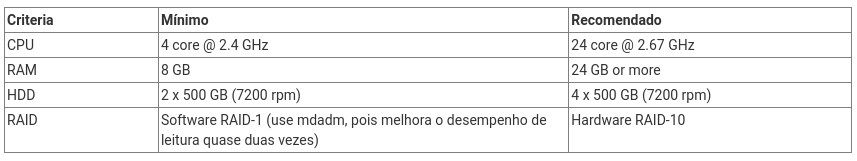
\includegraphics[width=0.9\textwidth]{images/hardware_requirements.png}
    \caption*{\textit{Fonte:} \url{https://docs.openstack.org/murano/rocky/admin/deploy_murano/prerequisites.html}.}
    \label{fig:hardware_requirements}
\end{figure}


\section{Arquitetura Geral}

Para implementar uma nuvem privada no campus do IFB, o \textit{cluster} OpenStack será composto por três nós: um nó principal (\textbf{Controller}), responsável pelos serviços essenciais, e dois nós adicionais dedicados, respectivamente, à criação de instâncias (\textit{Compute}) e ao armazenamento (\textit{Storage}). Essa divisão funcional segue o princípio de modularidade, conferindo escalabilidade e organização à arquitetura.

O \textbf{Controller} gerencia os demais nós do \textit{cluster}, centralizando a criação e administração de recursos. As configurações principais do OpenStack são definidas no arquivo \texttt{globals.yaml}, localizado em \texttt{/etc/kolla/globals.yaml}, que especifica os serviços executados, interfaces de rede e alocações de IP, incluindo o Neutron. Configurações adicionais, como a relação entre os nós, são feitas no arquivo \texttt{multinode}, encontrado em \texttt{venv/share/kolla-ansible/ansible/inventory/multinode}.

\begin{figure}[htbp]
    \centering
    \caption{Arquitetura geral do cluster OpenStack no IFB, mostrando a distribuição dos nós: \textbf{Controller}, responsável pelos serviços essenciais; \textbf{Compute}, para criação de instâncias; e \textbf{Storage}, dedicado ao armazenamento. A figura ilustra a relação funcional e as conexões entre os componentes.}
    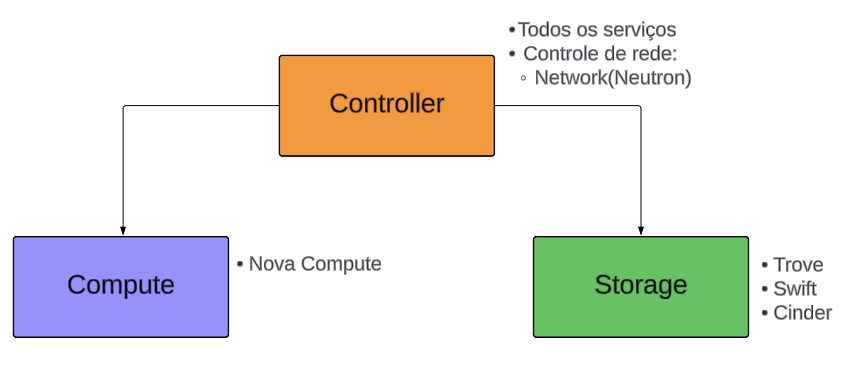
\includegraphics[width=0.7\textwidth]{images/cluster_architecture.png}
    \label{fig:cluster_architecture}
\end{figure}

Apesar de simples, essa arquitetura atende a todos os requisitos que comentamos sobre o campus, permitindo a criação de usuários, alocação de projetos e gerenciamento automatizado de recursos com agilidade. Além disso, o monitoramento detalhado possibilita tomadas de decisão informadas e a adição de recursos específicos para atender a demandas crescentes, garantindo flexibilidade e desempenho.

\section{Controller}

Devido às limitações do hardware, composto por servidores antigos com 16 GB de RAM e 120 GB de armazenamento total por nó, a configuração busca otimizar os recursos disponíveis. Essa capacidade é muito inferior à recomendada, mas é suficiente para executar o OpenStack em um ambiente de testes.

Uma limitação significativa é a ausência de discos dedicados exclusivamente a serviços de armazenamento como o \textbf{Swift} e o \textbf{Cinder}, que requerem volumes lógicos preferencialmente alocados em discos separados. No entanto, nesta configuração, todos os serviços operam em conjunto no mesmo ambiente.

\subsection{Ambiente de Teste com VMs}
Também foram realizados testes em VMs para compreender a arquitetura, sua conectividade e o gerenciamento. Esses testes se mostraram eficientes facilitando o controle e os ajustes necessários, proporcionando um ambiente flexível para experimentação. A seguir, é apresentada uma explicação simplificada sobre como essa arquitetura de teste foi configurada.

Para garantir estabilidade, as VMs foram configuradas com 18 GB de RAM, adequadas para suportar serviços críticos, como o sistema de filas. O nó \textbf{Controller} utiliza 4 vCPUs, enquanto os nós de \textit{compute} e \textit{storage} operam com 3 vCPUs cada. Apesar de ocasionais momentos de lentidão, essa configuração atende à demonstração proposta.

O \textbf{Controller} foi equipado com 120 GB de armazenamento para maior estabilidade, enquanto os demais nós utilizam 60 GB, suficientes para o propósito do teste. Em ambientes de produção, o nó de \textit{storage} demandaria uma maior capacidade de armazenamento para gerenciar grandes volumes de dados, e o nó de \textit{compute} necessitaria de mais memória RAM e processadores mais robustos para múltiplas instâncias simultâneas, a quantidade extada vai depender diretamente da quantidade de infraestrutura que será provida pelo campus.

Adicionalmente, dois discos extras foram alocados ao \textbf{Controller} para gerenciar \textit{storage}: um dedicado ao \textbf{Swift (Object Storage)} e outro ao \textbf{Cinder (Block Storage)}. A configuração desses discos é realizada no \texttt{globals.yaml}, sendo necessário criar os volumes lógicos previamente.

Embora o \textbf{Controller} gerencie serviços de armazenamento, um nó dedicado ao \textit{storage} pode ser adicionado ao \textit{cluster} para balancear a carga. O OpenStack distribui os dados automaticamente entre os nós disponíveis, permitindo escalabilidade conforme necessário, com adição eficiente de novos nós para atender ao crescimento das demandas.



\subsection{Configurações do Host OpenStack}

Como mencionado anteriormente, é fundamental compreender o papel dos volumes lógicos utilizados no \textit{cluster}, pois eles simplificam significativamente o gerenciamento de espaço. Com o uso de volumes lógicos, alterações como adicionar, remover ou modificar \textit{HDs} podem ser realizadas de forma transparente, sem a necessidade de alterar as configurações do \textit{cluster} OpenStack. Toda a manipulação ocorre diretamente nos volumes lógicos, garantindo maior flexibilidade e praticidade na administração dos recursos.

O nó \textbf{Controller} exige pelo menos duas interfaces de rede: uma para conexão interna e outra para conexão externa. No entanto, como não há uma conexão externa disponível para provisionar IPs públicos, utilizaremos as duas interfaces de forma diferente. Uma delas será dedicada ao Neutron, mas sem suporte para alocar IPs públicos diretamente às instâncias. Ainda assim, será possível utilizar o gateway padrão do \textit{switch} tendo acesso a internet e sendo possível que todos os usuários da rede interna acessem e utilizem as instâncias normalmente.

No caso da implementação em VMs, utilizaremos também duas interfaces porem configuradas para executar em modo \texttt{bridge}:
\begin{itemize}
    \item A primeira interface será configurada em modo \textit{bridge} com o host para permitir a comunicação interna.
    \item A segunda interface também será em modo \textit{bridge}, dedicada ao serviço \textbf{Neutron}, responsável por prover \textit{Network as a Service} (NaaS).
\end{itemize}

Os endereços IP estáticos para essas interfaces devem ser definidos no \texttt{netplan}. Configurar IPs fixos para os nós é essencial, pois no arquivo \texttt{multinode} é necessário especificar o IP ou o DNS do nó que será utilizado nos grupos de controle. Além disso, é necessário reservar um endereço IP exclusivo na rede para o \textbf{\textit{Kolla Internal VIP Address}}, utilizado na comunicação interna entre os serviços do OpenStack. A configuração deve ser como a mostrada em Código \ref{code:globals_vip_address}.

\begin{listing}[h!]
    \noindent\fcolorbox{black}{gray!10}{%
    \parbox{\textwidth}{%
      \inputminted[]{yaml}{files/globals_vip_address.yaml}
    }%
  }  
  \caption{Exemplo de configuração do endereço VIP interno e externo do Kolla no arquivo \texttt{globals.yaml}. Essa configuração inclui a definição das interfaces de rede (\texttt{network\_interface} e \texttt{neutron\_external\_interface}) e o \texttt{kolla\_internal\_vip\_address}, que deve ser um endereço IP exclusivo e não alocado, utilizado para a comunicação interna entre os serviços do OpenStack.}
  \label{code:globals_vip_address}
\end{listing}

O parâmetro \texttt{kolla\_base\_distro} é utilizado para especificar a distribuição do sistema operacional em que os serviços do OpenStack serão executados. Essa configuração auxilia o OpenStack a determinar quais pacotes devem ser instalados e como gerenciá-los dentro do cluster.

\subsection{Configuração de Rede}
A configuração da rede no OpenStack é um dos aspectos mais críticos para o funcionamento de um \textit{cluster}, pois garante a conectividade entre os nós e permite que as instâncias interajam com redes internas e externas. Uma rede bem configurada é essencial para a comunicação entre serviços, o acesso a recursos externos.

\subsection{Configuração de Rede Externa}
A configuração de uma rede externa no OpenStack é essencial para permitir o acesso a recursos fora do \textit{cluster} e para possibilitar a comunicação das instâncias com redes públicas ou corporativas. Esse processo inclui a definição da interface de rede física (ou virtual, no caso de VMs) responsável pela conexão externa, bem como a configuração do \textit{gateway} e do roteamento de tráfego. Após essa etapa, é necessário criar a rede externa e a sub-rede correspondente (\textit{subnet pool}), definindo a faixa de IPs públicos disponíveis, utilizando o \textit{Horizon} ou a \textit{CLI}.

Antes de iniciar a configuração, os seguintes pré-requisitos devem ser atendidos:
\begin{itemize}
    \item Identificar e definir a interface de rede a ser utilizada para a conexão ao meio externo.
    \item Alocar previamente os endereços IP públicos e a máscara de rede correspondente.
    \item Configurar o \textit{gateway} padrão e validar as regras do \textit{firewall}, garantindo que o tráfego necessário esteja permitido.
\end{itemize}

No caso de testes realizados em máquinas virtuais, é necessário configurar uma interface de rede no modo \textit{bridge}. Essa interface deve ser a mesma especificada no arquivo de configuração \texttt{globals.yaml} para o Neutron. Essa configuração garante que o tráfego da interface \texttt{br-ex} seja corretamente encaminhado para a rede externa, permitindo o acesso à internet pelas instâncias. 

Além disso, independentemente da forma de \textit{deployment}, se você estiver utilizando o \textbf{OVS} para controle de rede, que é o padrão do OpenStack, é crucial verificar se os parâmetros \texttt{local\_ip} e \texttt{bridge\_mappings} estão configurados corretamente no arquivo \texttt{openvswitch\_agent.ini}, como em Código \ref{code:config_openvswitch}.


\begin{listing}[h!]
    \noindent\fcolorbox{black}{gray!10}{%
    \parbox{\textwidth}{%
      \inputminted[]{ini}{files/config_openvswitch.ini}
    }%
  }  
  \caption{Configuração do arquivo \texttt{openvswitch\_agent.ini} para habilitar o suporte à rede no cluster utilizando o OpenvSwitch (\textbf{OVS}). Os parâmetros \texttt{bridge\_mappings} e \texttt{local\_ip} são essenciais para associar as redes físicas às pontes virtuais e definir o IP local do nó no cluster.}
  \label{code:config_openvswitch}
\end{listing}

\subsection{SSH Entre os Nós}
A configuração do acesso SSH é necessária na conexão dos nós, pois permite que o host principal gerencie e execute comandos em todo o \textit{cluster}.

Para configurar o acesso SSH, é necessário criar uma chave SSH no \textbf{controller} e garantir que ele tenha acesso com permissões de \textit{root} a todos os outros nós do \textit{cluster}. Essa configuração elimina a necessidade de fornecer senhas para executar comandos com privilégios elevados, simplificando a administração e automação.

O processo envolve copiar a chave pública gerada no \textbf{controller} para cada nó utilizando o comando \texttt{ssh-copy-id}. Após isso, o usuário configurado geralmente já terá acesso como \textit{sudo}. Caso contrário, será necessário acessar o nó, editar o arquivo de permissões utilizando o comando \texttt{visudo}, e adicionar o usuário do \textbf{controller} à lista de usuários com permissões de \textit{root}. Essa configuração garante que o \textbf{controller} possa gerenciar os nós de forma segura e com o acesso necessário.


\subsection {Containers do Cluster}
Dentro do Openstack a configuração do \textbf{Docker Compose} feito pelo kolla-ansible utiliza da tag \textit{`restart.always`} isso garante que se o container sofre com algum tipo de travamento e for deletado automaticamente o docker vai tentar subir outro container igual para tentar substituir ele. Isso é de extrema importância para manter a saúde do cluster e garantir que todos o serviços vão se manter de pé mesmo que ocorra algum tipo de travamento do container.

Essa política também é seguida pelas configurações de saúde do cluster chamado de \textit{healthcheck} garantindo que os containers sejam automaticamente recriados se forem removidos ou pararem, nesse caso até se o nó sofrer algum tipo de \textit{reboot} ele vai voltar criando os containers. Essas configurações podem ser vistas dentro de `/etc/kolla/docker-compose`. Obviamente para isso funcionar o serviço do docker precisa está executando se for parado forçadamente os containers também serão destruídos.

\subsection{Docker Register}
Antes de irmos para a criação do próximo nó é necessário criar um serviço de registro no \textit{controller}, ele basicamente vai ser responsável por fornecer as imagens dos serviços para os outros nós, dessa forma garantimos a consistência das imagens em todo o cluster \url{https://docs.openstack.org/kolla-ansible/latest/user/multinode.html}. Pode ser criado mais de um registro dentro do cluster, assim como pode ter vários \textit{controllers}. No nosso caso apenas um já resolve o problema. No \texttt{globals.yaml} devemos adicionar as variáveis como mostrado em Código \ref{code:docker_registry_globals}.

\begin{listing}[h!]
    \noindent\fcolorbox{black}{gray!10}{%
    \parbox{\textwidth}{%
      \inputminted[]{yaml}{files/docker_registry_globals.yaml}
    }%
  }  
  \caption{Configuração do \texttt{globals.yaml} para definir o \texttt{Docker registry} interno, especificando as variáveis necessárias para que o registro forneça as imagens de forma consistente aos demais nós do cluster.}
  \label{code:docker_registry_globals}
\end{listing}


Após subir o Docker Registry e enviar as imagens para ele, é necessário alterar o arquivo \texttt{/etc/docker/daemon.json} no Docker para direcionar o \textit{pull} das imagens primeiramente ao serviço de registro configurado no \textbf{Controller}. Isso garante que, ao adicionar novos nós ao cluster, eles busquem as imagens diretamente do registro interno, assegurando a consistência das imagens. Além disso, essa configuração facilita a propagação de novas imagens no cluster, tornando o processo mais eficiente e controlado. Dentro das configurações do Docker no arquivo \texttt{deamon.json} deve se adicionar Código \ref{code:docker_insecure_registry}.


\begin{listing}[h!]
    \noindent\fcolorbox{black}{gray!10}{%
    \parbox{\textwidth}{%
      \inputminted[]{json}{files/docker_insecure_registry.json}
    }%
  }  
  \caption{Configuração do arquivo \texttt{daemon.json} para incluir o registro interno no Docker como uma rota insegura (\textit{http}), permitindo que os nós do cluster realizem o \textit{pull} das imagens diretamente do \texttt{Docker registry} interno.}
  \label{code:docker_insecure_registry}
\end{listing}


\subsection{Configuração Multinode}
Para finalizar, é necessário ajustar o arquivo de configuração do Kolla-Ansible, chamado \textbf{multinode}, para especificar de forma clara quais serviços estão associados a cada nó do cluster. Nesta configuração, os serviços são organizados em grupos, como o \textbf{[Controler]}. No nosso caso, adicionamos o segundo nó ao grupo \textbf{[Storage]}. Essa definição no arquivo \textbf{multinode} garante que o \textbf{Controller} saiba exatamente onde cada serviço deve ser instalado e como acessar os demais nós. O arquivo \textbf{multinode} deve seguir o formato ilustrado no Código \ref{code:config_multinode}.

\begin{listing}[h!]
    \noindent\fcolorbox{black}{gray!10}{%
    \parbox{\textwidth}{%
      \inputminted[]{ini}{files/config_multinode.ini}
    }%
  }  
  \caption{Configuração do arquivo multinode separando os grupos de controle entre os nós.}
  \label{code:config_multinode}
\end{listing}

Caso seja necessário criar variáveis de ambiente ou configurar caminhos padrões do openstack, como o caminho do \textbf{python} que será utilizado, pode-se alterar o arquivo \textbf{ansible.cfg} naturalmente encontrado em \textit{`~/ansible/`}, caso não tenha sido criado pelo \textbf{deployment} do \textit{multinode}, não tem problema criar o arquivo direto em `~/.ansible.cfg`. 

Para verificar se o OpenStack está utilizando o arquivo de configuração correto, pode-se executar o comando `ansible --version`:

\section{Segundo Nó (Storage)}

Este nó será dedicado exclusivamente ao armazenamento, utilizando os serviços \textbf{Cinder} e \textbf{Swift}, cada um alocado em \textit{volume groups} separados. Inicialmente, cada \textit{volume group} (\texttt{cinder-volumes} e \texttt{swift-volumes}) será configurado com um único disco. Essa abordagem oferece flexibilidade para futuras expansões, permitindo adicionar novos discos ao \textit{volume group} sem complexidade significativa.

A criação inicial dos \textit{volume groups} é realizada manualmente no \textbf{Controller}, que também executa todos os serviços essenciais. Dessa forma, é necessário alocar previamente os discos destinados ao \textbf{Swift} e ao \textbf{Cinder} no \textbf{Controller} antes de configurar o nó de \textit{storage}. Após essa etapa, é possível automatizar a criação de volumes e a configuração dos discos, reduzindo a necessidade de intervenção manual nos nós. Caso novos discos sejam adicionados após a implantação inicial, eles podem ser incluídos manualmente nos \textit{volume groups} do nó de \textit{storage} de forma simples e eficiente.

Uma vez configurado o \textbf{Controller}, é essencial garantir que ele tenha acesso ao nó de \textit{storage}. Isso requer a configuração das chaves SSH para permitir o acesso seguro e direto do \textbf{Controller} ao nó de \textit{storage}, eliminando a necessidade de autenticação manual. Além disso, é necessário atualizar o arquivo de inventário \texttt{/etc/kolla/inventory/multinode} com o endereço IP ou DNS do nó de \textit{storage}, garantindo que os serviços do OpenStack possam localizá-lo corretamente.

Com o nó de \textit{storage} configurado, o \textbf{Cinder} gerenciará volumes para instâncias e o \textbf{Swift} será responsável pelo armazenamento de objetos, permitindo que o \textit{cluster} atenda a diferentes demandas de armazenamento de maneira eficiente e escalável.


\section{Terceiro Nó (Compute)}

Este nó será dedicado exclusivamente à criação de máquinas virtuais (\textit{instances}), desempenhando o papel equivalente ao EC2 em provedores de nuvem pública. Ele utilizará os recursos alocados, como CPU, memória e armazenamento local, para provisionar máquinas virtuais com base nos \textit{flavors} definidos pelo usuário da organização.

Os \textit{flavors} representam as especificações das máquinas virtuais, como quantidade de CPUs, memória RAM e tamanho do disco. Esses recursos são consumidos diretamente do nó \textbf{Compute}, que é responsável por executar as instâncias e garantir sua performance, isolação e conectividade.

A configuração do nó \textbf{Compute} é realizada pelo Kolla-Ansible, utilizando o arquivo de inventário \texttt{/etc/kolla/inventory/multinode}. Neste arquivo, o nó \textbf{Compute} deve ser listado sob o grupo \textbf{[compute]} para que os serviços necessários, como o \textit{Nova Compute}, sejam implantados corretamente. Além disso, o \textbf{Controller} gerencia as tarefas administrativas relacionadas à criação, inicialização e destruição das máquinas virtuais, enquanto o nó \textbf{Compute} executa as operações físicas.

A comunicação entre o \textbf{Controller} e o nó \textbf{Compute} é feita de forma segura e direta. Seguindo a mesma ideia do outro nó precisamos configurar a chave ssh e adicionar o DNS ou IP no \textbf{multinode}

Após a implantação inicial, o nó \textbf{Compute} estará pronto para receber solicitações de criação de máquinas virtuais. Ele será responsável por alocar os recursos conforme especificado nos \textit{flavors}, garantindo a escalabilidade e eficiência do \textit{cluster}. Caso novos nós \textbf{Compute} sejam adicionados ao \textit{cluster}, o balanceamento de carga entre os nós será automaticamente gerenciado pelo OpenStack, otimizando o uso de recursos.


\section{\textit{Deploy} da Aplicação}
Após configurar a rede e os arquivos mencionados, o \textit{deploy} dos serviços pode ser realizado. Esse processo cria múltiplos contêineres que executam os serviços padrão do OpenStack, conforme ilustrado na Figura \ref{fig:controller_containers}. O acesso ao painel do OpenStack (\textbf{Horizon}) pode ser feito por meio do endereço \texttt{http://kolla\_internal\_vip\_address/dashboard}. A partir desse painel, é possível configurar todos os serviços de \textit{Infrastructure as a Service} (IaaS). Detalhes adicionais sobre a configuração dos serviços serão apresentados nas próximas seções.


\begin{figure}[htbp]
    \centering
    \caption{Containers de base do serviço OpenStack executando no nó principal do cluster após efetuar o deploy com o kolla-ansible, mostrando de estão saudáveis e quando foram iniciados}
    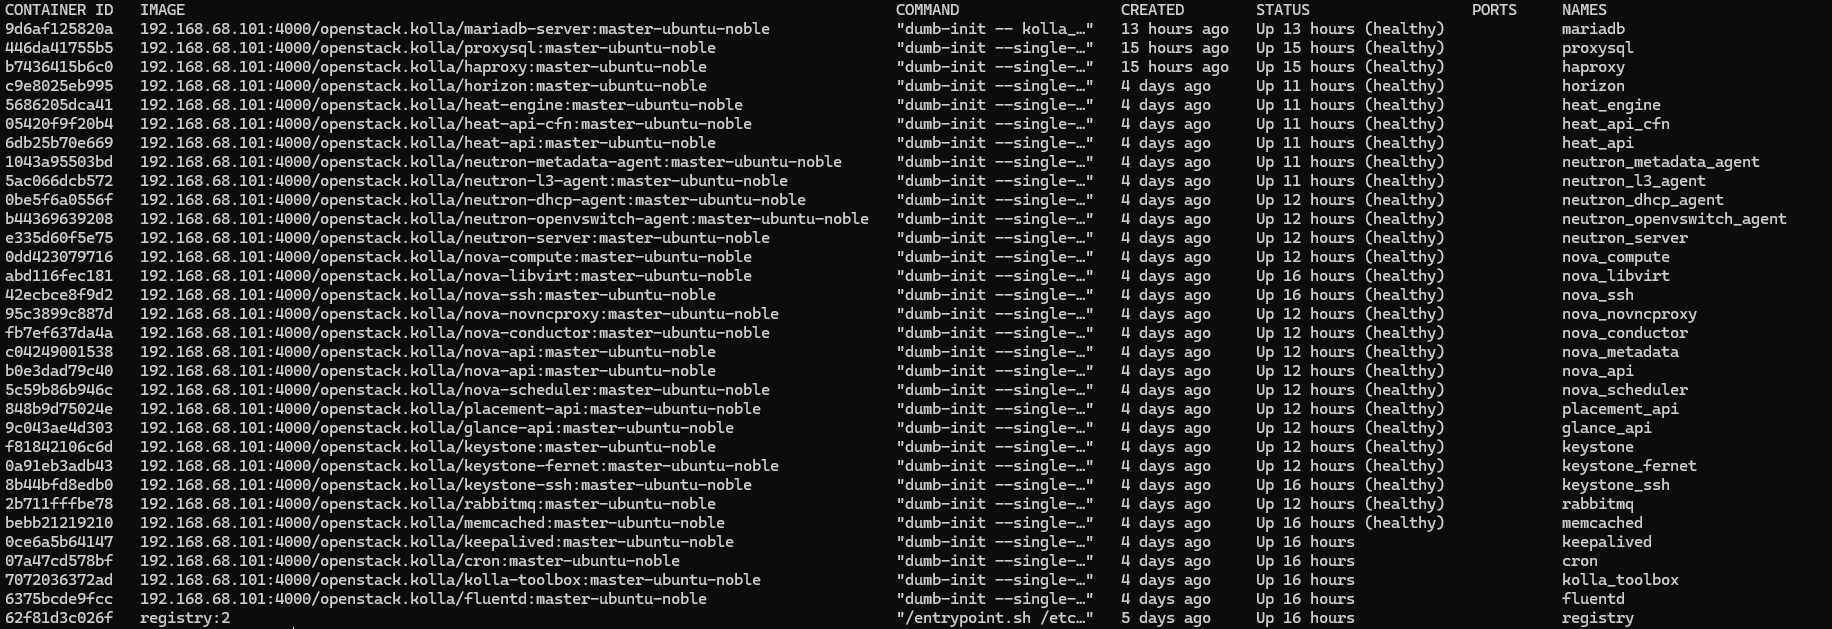
\includegraphics[width=1.0\textwidth]{images/controller_containers.png}
    \caption{Imagem retirada do terminal do nó principal do cluster}
    \label{fig:controller_containers}
\end{figure}

Os contêineres exibidos, ou a maioria deles, devem estar visíveis em todos os nós do cluster. Cada contêiner possui a tag \textit{health}, indicando que está em execução sem erros detectados.

\section{Por Dentro do OpenStack}
Depois de configurado o \textit{cluster}, é fundamental entender a forma como o OpenStack organiza e gerencia seus recursos. O OpenStack funciona por meio de \textbf{projetos}, que podem conter diversos \textbf{usuários}, e cada usuário tem permissões específicas definidas pelas \textit{roles}. 

A seguir, exploraremos os principais conceitos e configurações relacionados aos projetos, usuários, políticas de acesso, cotas e rede, detalhando suas funcionalidades e como interagem no ecossistema OpenStack, todos os comandos mostrados podem ser feitos direto pelo Horizon.

\subsection{OpenStack-Client}
Para utilizar a maioria dos comandos descritos nesta seção, é necessário instalar o pacote python-openstackclient. Isso pode ser feito utilizando o gerenciador de pacotes pip. Após a instalação, você deve realizar o login configurando as variáveis de ambiente listadas abaixo.

Por padrão, as únicas alterações necessárias serão no valor de `VIP\_IP` (o endereço IP configurado) e na senha gerada automaticamente. O endereço IP pode ser consultado no arquivo \texttt{globals.yaml}, enquanto a senha pode ser obtida utilizando o comando da Figura~\ref{code:grep_password}.

\begin{listing}[h!]
    \noindent\fcolorbox{black}{gray!10}{%
    \parbox{\textwidth}{%
      \inputminted[]{sh}{files/grep_password.sh}
    }%
  }  
  \caption{Comando utilizado para recuperar a senha gerada automaticamente para a conta \texttt{admin} no arquivo de configuração do Kolla (\texttt{passwords.yml}). Essa senha será utilizada para configurar o acesso ao OpenStack.}
  \label{code:grep_password}
\end{listing}

Após obter essas informações, é possível criar o arquivo \texttt{admin\_variables.sh}, que conterá as variáveis de ambiente necessárias para acessar o \textit{admin}. Depois de criar esse arquivo com as variáveis demonstradas na Figura~\ref{code:source_admin}, basta executá-lo com o comando \texttt{source admin\_variables.sh}

\begin{listing}[h!]
    \noindent\fcolorbox{black}{gray!10}{%
    \parbox{\textwidth}{%
      \inputminted[]{sh}{files/source_admin.sh}
    }%
  }  
  \caption{Exemplo de configuração das variáveis de ambiente necessárias para acessar o \texttt{admin} do OpenStack utilizando o Terminal. Inclui definições do endpoint (\texttt{OS\_AUTH\_URL}), credenciais de autenticação, e outros parâmetros essenciais.}
  \label{code:source_admin}
\end{listing}

\subsection{Projetos}
Os projetos (também chamados de \textit{tenants}) agrupam recursos como instâncias, redes e volumes. Cada projeto possui isolamento de recursos, evitando interferência de um projeto sobre outro. Além disso, é possível definir cotas para limitar o uso de instâncias, redes e outros recursos. Cada projeto pode ter usuários com papéis bem definidos, garantindo um controle de acesso eficaz.

O OpenStack também permite personalizar quais serviços um projeto pode acessar, como \textit{Swift}, \textit{Glance}, entre outros. Na figura \ref{fig:openstack_projects}, é exibida a interface do dashboard Horizon, onde podem ser realizadas as configurações relacionadas a projetos, incluindo sua criação e atribuição de permissões.

\begin{figure}[htbp]
    \centering
    \caption{Interface do Horizon mostrando a configuração e gerenciamento de projetos, local onde também é configurado todos os detalhes relacionados aos projetos.}
    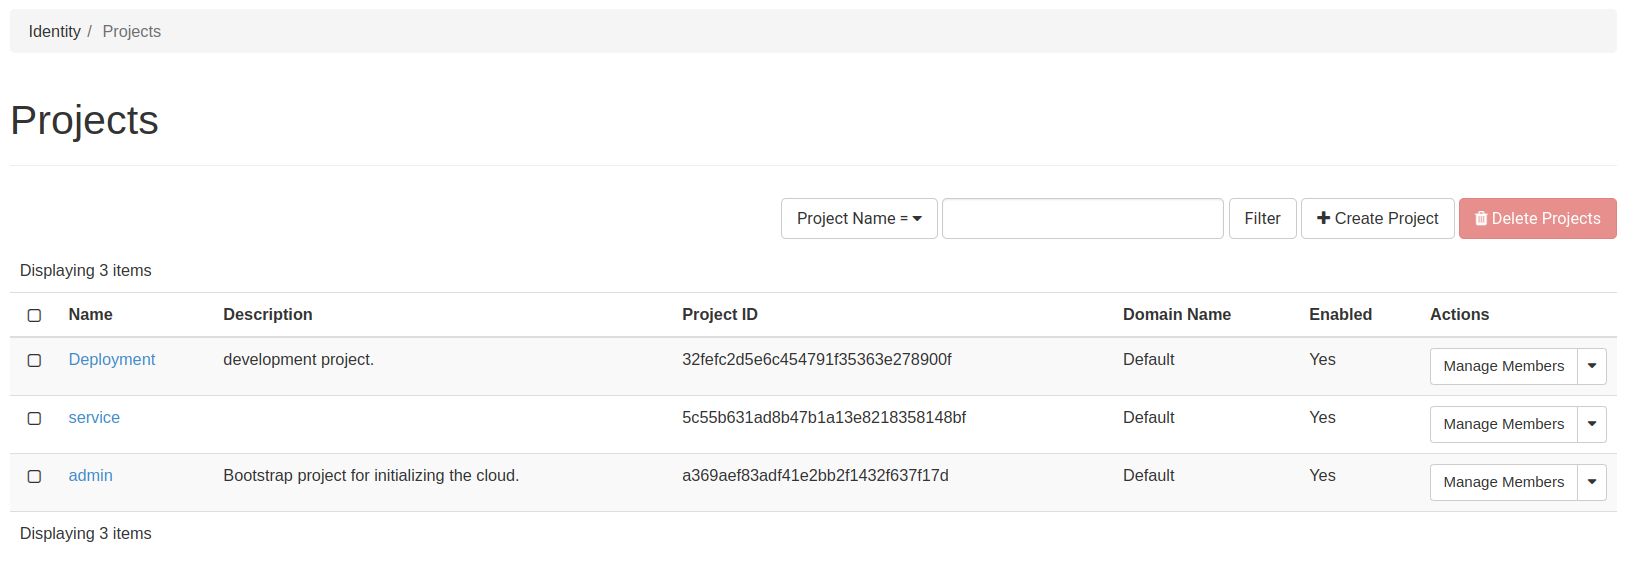
\includegraphics[width=0.9\textwidth]{images/openstack_projects.png}
    \caption*{Fonte: Dashboard Horizon do OpenStack.}
    \label{fig:openstack_projects}
\end{figure}

Dentro dos projetos utilizamos cotas. As cotas delimitam o número de recursos que cada projeto pode consumir, como instâncias, volumes e redes. Embora sejam úteis para evitar o uso abusivo de recursos, o OpenStack não garante previamente que o \textit{cluster} tenha a capacidade de suprir todas as cotas aprovadas. Caso um projeto tente criar recursos além da capacidade disponível no \textit{cluster}, erros de criação podem ocorrer, e nós sobrecarregados podem apresentar \textit{reboots} inesperados.

\subsection{Usuários}
Os usuários são entidades autenticadas pelo serviço \textbf{Keystone}, que gerencia identidades e permissões. Eles podem ser criados tanto pela interface de linha de comando (CLI) quanto pela interface gráfica (Horizon). Cada usuário está associado a um ou mais projetos, com \textit{roles} específicas que definem suas permissões dentro do ambiente.

O Keystone oferece suporte a diferentes métodos de autenticação, como LDAP ou banco de dados interno, permitindo integração com sistemas externos. Na figura \ref{fig:openstack_users}, é mostrado como usuários e contas de serviço são configurados de forma similar, diferenciando-se apenas pelas políticas de segurança atribuídas.

\begin{figure}[htbp]
    \centering
    \caption{Interface do Horizon mostrando usuários e contas de serviço configurados pelo Keystone.}
    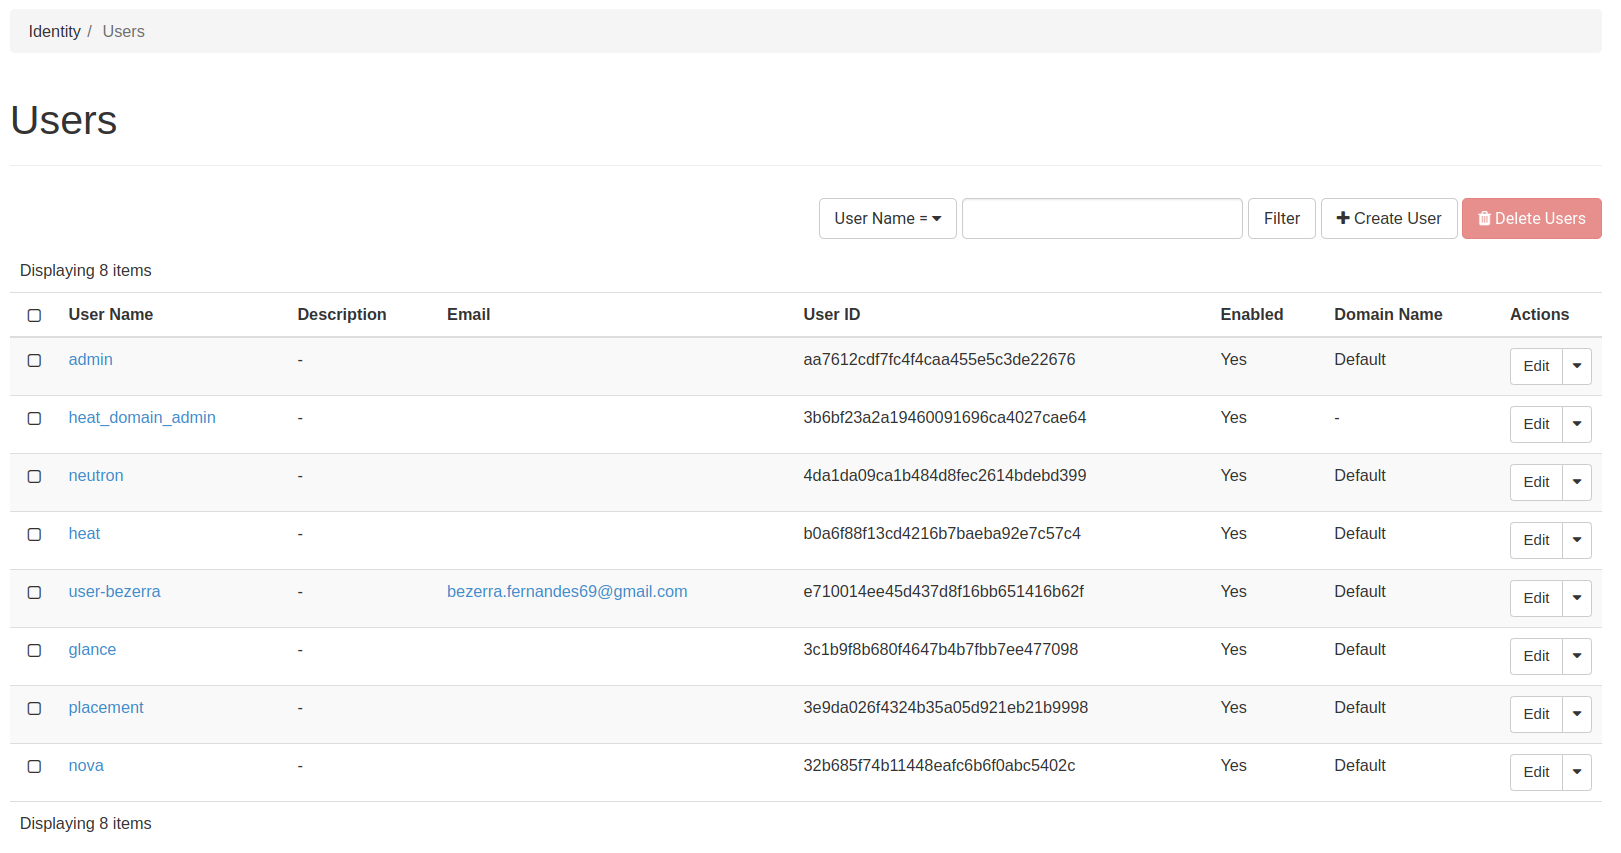
\includegraphics[width=0.9\textwidth]{images/openstack_users.png}
    \caption*{Fonte: Dashboard Horizon do OpenStack.}
    \label{fig:openstack_users}
\end{figure}

\subsection{Políticas de Acesso para Serviços e Usuários}
As políticas de acesso, definidas em arquivos de configuração (JSON ou YAML), determinam quais operações cada \textit{role} pode executar nos serviços, como \textit{Nova}, \textit{Neutron} e \textit{Cinder}. Isso viabiliza um controle granular, permitindo personalizar ações como criação de instâncias e gerenciamento de redes.

Em implantações como \textit{Kolla-Ansible}, esses arquivos podem ser gerenciados centralmente para simplificar a administração. Na figura \ref{fig:openstack_roles}, são mostradas as \textit{roles} padrão criadas pelo OpenStack para contas de serviço.

\begin{figure}[htbp]
    \centering
    \caption{Interface do Horizon mostrando as \textit{roles} padrões do OpenStack para controle de contas de serviço.}
    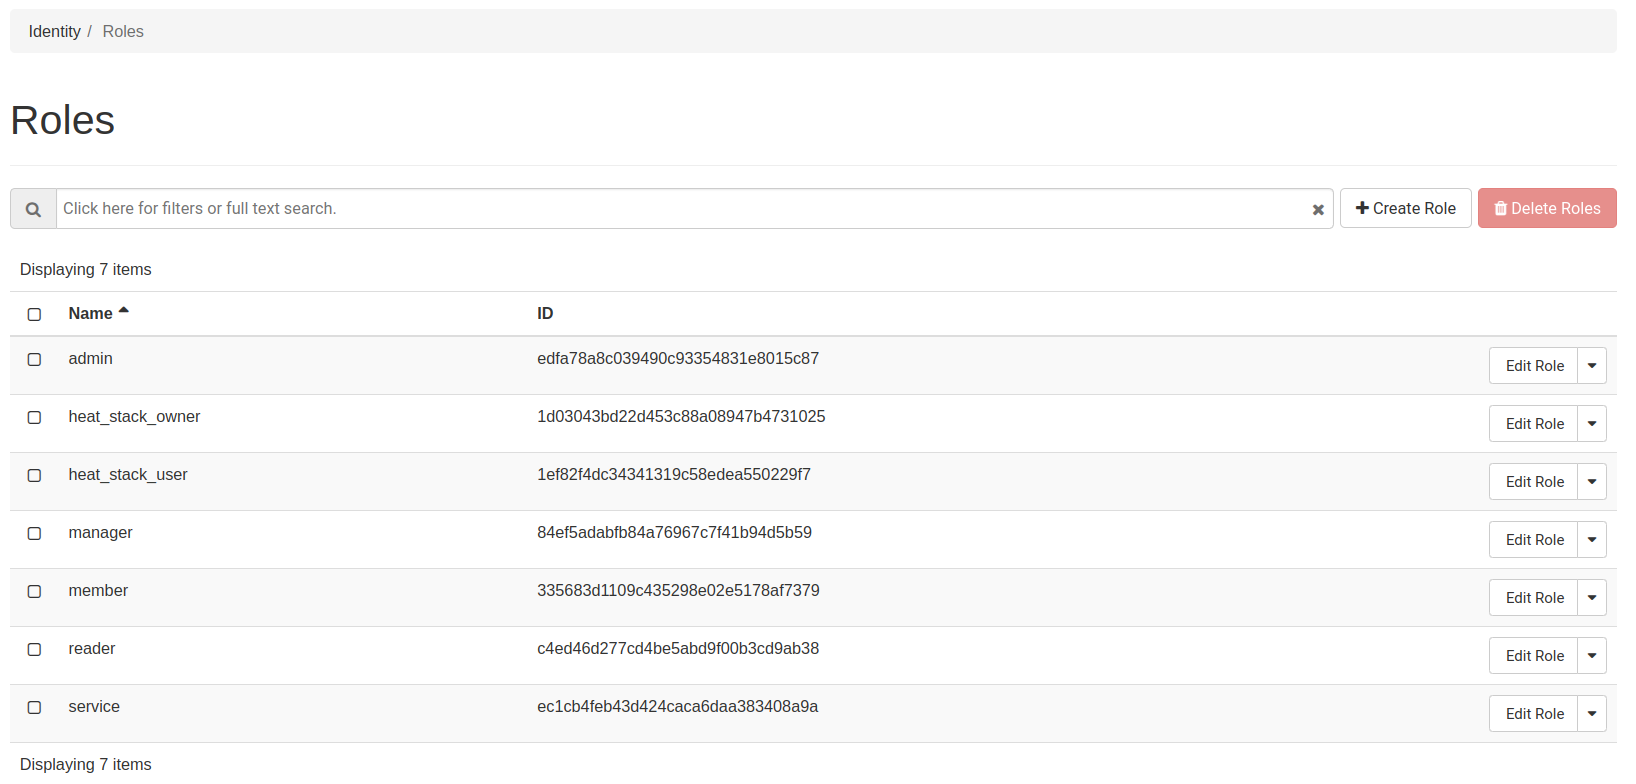
\includegraphics[width=0.9\textwidth]{images/openstack_roles.png}
    \caption*{Fonte: Dashboard Horizon do OpenStack.}
    \label{fig:openstack_roles}
\end{figure}

\subsection{Rede}
O serviço \textbf{Neutron} gerencia a criação de redes e \textit{subnets} virtuais (ou VPCs), onde se definem regras de firewall, roteamento e conexões entre instâncias. Cada projeto pode manter suas próprias redes isoladas, garantindo segurança e organização.

A visualização da topologia de rede no Horizon (ou via \textit{CLI}) exibe como cada elemento (instâncias, roteadores e sub-redes) está interligado, ajudando a identificar rotas e possíveis pontos de falha. Após as configurações iniciais, é possível criar uma rede externa utilizando os seguintes comandos em Código \ref{code:command_external_network}.

\begin{listing}[h!]
    \noindent\fcolorbox{black}{gray!10}{%
    \parbox{\textwidth}{%
      \inputminted[]{sh}{files/command_external_network.sh}
    }%
  }  
  \caption{Comandos para criar uma rede externa no OpenStack. A configuração define o tipo de rede (\texttt{flat}), associa a rede ao provedor físico (\texttt{physnet1}), e configura uma sub-rede com intervalo de endereços alocados, gateway e desativação do DHCP.}
  \label{code:command_external_network}
\end{listing}

Nesse exemplo, criamos a \textit{network} externa e definimos uma \textit{subnet} para alocar IPs no intervalo especificado em \textbf{--allocation-pool}, além de configurarmos o \textit{gateway} de saída.

Em seguida, criamos uma rede interna, que será utilizada pelas instâncias. Enquanto a rede externa é compartilhada entre projetos, as redes internas são isoladas para cada projeto, sendo criadas a partir de contas administradoras de projetos:

\begin{listing}[h!]
    \noindent\fcolorbox{black}{gray!10}{%
    \parbox{\textwidth}{%
      \inputminted[]{sh}{files/command_internal_network.sh}
    }%
  }  
  \caption{Comandos para criar uma rede interna no OpenStack. Redes internas são isoladas por projeto e utilizadas pelas instâncias. A configuração inclui a criação da rede e de uma sub-rede associada, com as definições de faixa de IPs, gateway e outras propriedades específicas.}
  \label{code:command_internal_network}
\end{listing}

Para verificar se as conexões foram configuradas corretamente, podemos acessar a área \textit{Network Topology}. Essa seção apresenta uma visualização gráfica de como a \textit{Network} está estruturada, permitindo identificar as conexões entre instâncias, roteadores e sub-redes. A figura \ref{fig:network_topology} ilustra essa visualização dentro do dashboard Horizon.

\begin{figure}[htbp]
    \centering
    \caption{Visualização da topologia de rede no dashboard Horizon, mostrando as conexões entre instâncias, roteadores e sub-redes.}
    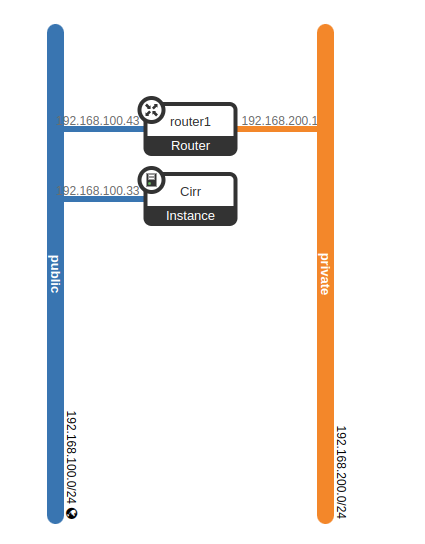
\includegraphics[width=0.5\textwidth]{images/network_topology.png}
    \caption*{Fonte: Dashboard Horizon do OpenStack.}
    \label{fig:network_topology}
\end{figure}

\subsection{Arquitetura de Separação de Recursos para o Campus}

O OpenStack oferece diversas formas de organizar e separar projetos e usuários para atender a diferentes necessidades. No contexto de uma instituição de ensino superior, como um campus universitário, é comum a necessidade de segmentar recursos entre departamentos, e dentro desses, entre seus respectivos usuários. Uma abordagem eficiente para essa finalidade é a utilização da \href{https://wiki.openstack.org/wiki/HierarchicalMultitenancy}{\textit{Hierarchical Multitenancy}}.

Essa arquitetura permite a criação de uma hierarquia de projetos, em que subprojetos são vinculados a um projeto principal. Cada projeto principal pode representar um departamento, como Engenharia, Ciências da Computação ou Administração, enquanto os subprojetos podem ser utilizados para atividades específicas, como Trabalhos de Conclusão de Curso (TCCs), pesquisas acadêmicas ou laboratórios de ensino. 

A utilização dessa arquitetura torna-se ainda mais poderosa quando combinada com os templates do Heat. Esses templates permitem a criação automatizada de todos os componentes necessários para iniciar uma nova pesquisa ou atividade, otimizando o provisionamento de recursos e reduzindo o esforço operacional. A seguir, serão apresentados detalhes sobre os templates e suas aplicações práticas.



\subsection{Debug e Resolução de Problemas}
Devido à complexidade e constante desenvolvimento do OpenStack, erros são situações frequentes e podem exigir diferentes abordagens de depuração. A análise inicial deve sempre incluir a verificação dos arquivos de log, geralmente localizados em \textbf{/var/log/kolla/}, que fornecem informações detalhadas sobre o comportamento dos serviços e possíveis falhas. Adicionalmente, habilitar o modo de depuração nos serviços pode facilitar a identificação de problemas. Isso pode ser feito configurando a variável \texttt{DEBUG=True} no arquivo de configuração do serviço em questão.

Quando o problema envolve um erro mais profundo, como falhas em componentes do código, recomenda-se o uso do \textbf{DevStack}. O DevStack é uma ferramenta leve e altamente configurável, ideal para criar um ambiente de desenvolvimento que replica uma instalação do OpenStack em um único nó. Ele permite a execução de serviços do OpenStack em modo debug, facilitando o acesso a logs detalhados e a inserção de pontos de interrupção no código. Esse ambiente é ideal para testar alterações e investigar problemas sem afetar a instalação principal.

Para realizar uma depuração interativa com o DevStack, pode-se utilizar o depurador \textit{pdb} do Python. Insere-se a seguinte linha no código no ponto onde deseja interromper a execução: \texttt{import pdb; pdb.set\_trace()}.

Após ajustar o código, basta reiniciar o serviço no ambiente DevStack para realizar a análise interativa. Essa abordagem é vantajosa, pois permite isolar problemas e testar soluções de forma controlada antes de aplicá-las em um ambiente de produção.

Embora a maioria dos erros possa ser resolvida ajustando configurações ou corrigindo permissões, erros de código mais profundos requerem conhecimento detalhado sobre o funcionamento interno dos serviços do OpenStack e suas interações. Nesses casos, o uso do DevStack como ambiente de desenvolvimento é altamente recomendado, pois proporciona flexibilidade e controle total sobre os serviços e suas dependências.

\section{Migração e Atualizações Futuras}

No contexto de software, atualizações e correções de erros são lançadas regularmente, e o OpenStack não é uma exceção. É fundamental manter o ambiente atualizado para aproveitar novos recursos (\textit{features}) e melhorias de desempenho, além de corrigir vulnerabilidades de segurança. Antes de realizar qualquer atualização, é de extrema importância garantir que todos os backups necessários estejam disponíveis, permitindo a restauração do sistema em caso de falhas.

\subsection{Atualização de Contêineres}

Como mencionado anteriormente, o Kolla-Ansible isola os serviços do OpenStack em contêineres Docker. Essa arquitetura permite atualizar os contêineres de forma individual. No entanto, para garantir que todos os serviços sejam devidamente sincronizados, se comuniquem corretamente e, quando necessário, sejam reconfigurados automaticamente, recomenda-se realizar uma atualização completa utilizando como Código \ref{code:update_kolla}:

\begin{listing}[h!]
    \noindent\fcolorbox{black}{gray!10}{%
    \parbox{\textwidth}{%
      \inputminted[]{sh}{files/update_kolla.sh}
    }%
  }  
  \caption{Comando para atualizar todos os serviços do OpenStack gerenciados pelo Kolla-Ansible. Essa abordagem garante que os contêineres sejam sincronizados, configurados corretamente e reconfigurados automaticamente quando necessário.}
  \label{code:update_kolla}
\end{listing}

Esse procedimento garante que os contêineres sejam atualizados para as versões mais recentes das imagens, aplicando automaticamente quaisquer modificações necessárias nas configurações e garantindo a continuidade dos serviços.

Em alguns casos, quando são lançadas novas \textit{features} ou alterações significativas nas configurações, é necessário atualizar o arquivo \texttt{globals.yaml}. Esse arquivo atualizado pode ser encontrado no diretório de exemplos \texttt{../kolla-ansible/etc\_examples/kolla/*}. Após obter o novo arquivo, é necessário incorporar manualmente as configurações existentes para preservar a compatibilidade com o ambiente atual.


\section{Análise do Cluster}

Com os três nós configurados e operacionais, utilizamos serviços nativos do OpenStack para realizar a análise do cluster. Os serviços utilizados incluem:

\begin{itemize}
    \item \textbf{Gnocchi}: Responsável por coletar e armazenar métricas relacionadas ao desempenho e utilização do cluster, como uso de CPU, memória e armazenamento.
    \item \textbf{Aodh}: Utilizado para a configuração de alarmes. Este serviço nos permite definir ações automatizadas caso ocorra alguma falha.
    \item \textbf{Panko}: Registro e armazenamento de logs de eventos, mostrando exatamente o que foi feito e por qual pessoa.
    \item \textbf{Ceilometer}: Um dos principais serviços do OpenStack para medição de dados de uso. Ele fornece uma visão abrangente dos recursos consumidos, contribuindo para relatórios detalhados e para a gestão eficiente do cluster.
\end{itemize}

A integração desses serviços permite não apenas monitorar o desempenho e a utilização do cluster, mas também detectar anomalias e registrar eventos críticos. Essa abordagem facilita a manutenção preventiva e corretiva no ambiente OpenStack.

Além disso, o \textbf{Ceilometer} permite integração com outros serviços de monitoramento amplamente utilizados, como o Grafana. Essa conexão possibilita a criação de dashboards personalizados para visualizar métricas em tempo real, identificar tendências de uso e acompanhar o desempenho do cluster de maneira gráfica e centralizada. 

Por fim, a análise do cluster é um passo essencial para garantir que a infraestrutura opere com alta disponibilidade, desempenho consistente e segurança, características fundamentais para atender às demandas de um ambiente acadêmico e administrativo.


\section{Implementação e Utilização de Recursos}
O Heat é o serviço de orquestração do OpenStack que permite automatizar o gerenciamento de infraestrutura por meio de templates declarativos escritos em YAML, naturalmente esse tipo de serviço é chamado de IaC  \textit{(Infraestructure as Code)}. Com ele, você pode definir, provisionar e gerenciar recursos, como instâncias, volumes, redes e até aplicações inteiras, de forma padronizada e repetível. Esse serviço é especialmente útil para configurar ambientes de trabalho para novos estudantes, permitindo que iniciem projetos com rapidez e eficiência. Além disso, o mesmo template pode ser facilmente ajustado para adicionar mais recursos, conforme a necessidade do projeto.

Os próprios alunos também podem utilizar templates do Heat para gerenciar a infraestrutura de seus projetos. Isso facilita a demonstração de quais recursos foram utilizados e como o ambiente pode ser replicado de forma simples e eficiente. Essa abordagem promove organização e consistência no uso dos recursos de infraestrutura, otimizando o aprendizado e a colaboração em projetos acadêmicos.

\subsection{Configuração para a utilização de IaC}
É possível que o serviço Heat não tenha permissões diretas para acessar e manipular o cluster. Para contornar essa limitação, normalmente criamos um arquivo de configuração específico para o Heat em /etc/kolla/config/heat.conf, utilizando a configuração como mostrado em Código \ref{code:heat_configuration}.

É altamente recomendável manter esses arquivos de configuração devidamente protegidos, pois eles geralmente contêm credenciais sensíveis. Essa prática deve ser aplicada a todos os arquivos localizados em /etc/kolla/, garantindo a segurança do ambiente e prevenindo acessos não autorizados.


\begin{listing}[h!]
    \noindent\fcolorbox{black}{gray!10}{%
    \parbox{\textwidth}{%
      \inputminted[]{sh}{files/heat_configuration.conf}
    }%
  }  
  \caption{Exemplo de configuração do arquivo \texttt{heat.conf}, localizado em \texttt{/etc/kolla/config/}. Esse arquivo define as permissões e parâmetros necessários para o serviço Heat gerenciar a infraestrutura no cluster.}
  \label{code:heat_configuration}
\end{listing}


\subsection{Criação de Instâncias para Alunos em Sala de Aula}

Uma aplicação prática do cluster em um ambiente acadêmico é sua integração com as atividades em sala de aula. Considere o seguinte cenário: você está ministrando uma aula sobre processamento de imagens e deseja disponibilizar uma instância para cada aluno. Essas instâncias podem ser configuradas previamente com um ambiente virtual e todos os pacotes necessários do Python já instalados, garantindo que os alunos possam se concentrar exclusivamente nos objetivos da aula.

Para alcançar esse objetivo, é possível utilizar um único template do Heat. Aplicando o conceito de \texttt{HierarchicalMultitenancy}, criamos um subprojeto denominado \texttt{aula-proc-dig} dentro do projeto principal. Nesse subprojeto, as instâncias dos alunos serão provisionadas de forma organizada Código \ref{code:template_heat_one}.

\begin{listing}[h!]
    \noindent\fcolorbox{black}{gray!10}{%
    \parbox{\textwidth}{%
      \inputminted[]{yaml}{files/template_heat_one.yaml}
    }%
  }  
  \caption{Exemplo de template Heat para provisionamento automatizado de instâncias no subprojeto \texttt{aula-proc-dig}, configuradas para atividades de processamento de imagens.}
  \label{code:template_heat_one}
\end{listing}

\newpage

\subsection{Criação de Projetos para Alunos de Pesquisa}

Para atender alunos que estão iniciando projetos de pesquisa, como CNPq ou Trabalhos de Conclusão de Curso (TCC), é possível criar um template dedicado. Também seguindo o conceito de \texttt{HierarchicalMultitenancy}, podemos provisionar uma rede e uma instância isolada para cada aluno, permitindo que eles configurem o ambiente de acordo com suas necessidades específicas. Além disso, essa abordagem facilita a escalabilidade, possibilitando a alocação de recursos adicionais de maneira ágil e controlada, caso seja necessário Código \ref{code:template_heat_two_part1}.

\begin{listing}[h!]
    \noindent\fcolorbox{black}{gray!10}{%
    \parbox{\textwidth}{%
      \inputminted[]{yaml}{files/template_heat_two_part1.yaml}
    }%
  }  
  \caption{Parte 1: Exemplo de template Heat para provisionamento de projetos individuais de pesquisa, incluindo uma rede e uma instância configurável, com suporte à escalabilidade de recursos, continuação em Código \ref{code:template_heat_two_part2}.}
  \label{code:template_heat_two_part1}
\end{listing}

\begin{listing}[h!]
  \noindent\fcolorbox{black}{gray!10}{%
  \parbox{\textwidth}{%
    \inputminted[firstnumber=26]{yaml}{files/template_heat_two_part2.yaml}
  }%
}  
\caption{Parte 2: Criação dos recursos do necessário para rodar as instâncias com a imagem escolhida em Código \ref{code:template_heat_two_part1}.}
\label{code:template_heat_two_part2}
\end{listing}



Esses templates foram projetados para atender às necessidades específicas dos alunos em atividades acadêmicas, mas a abordagem é flexível e pode ser adaptada para qualquer membro do campus que necessite de infraestrutura computacional. Professores, pesquisadores e equipes administrativas podem solicitar recursos personalizados, como instâncias, redes ou ambientes configurados, que serão provisionados de forma automatizada e organizada por meio de templates do Heat.
  \chapter{Conclusão}


\section{Panorama Geral e Viabilidade do Projeto}
A proposta de implementação de uma nuvem privada no Instituto Federal de Brasília (IFB), detalhada ao longo deste trabalho, demonstrou-se promissora e possível para atender às demandas acadêmicas e administrativas da instituição. Baseada no OpenStack e utilizando \textit{Kolla-Ansible} para a conteinerização dos serviços, a arquitetura aqui descrita destaca-se pela flexibilidade e escalabilidade, podendo se adaptar a cenários de maiores dimensões e complexidades. Este trabalho apresentou uma análise detalhada das tecnologias envolvidas, destacando o OpenStack como a solução mais adequada para atender às demandas específicas de escalabilidade.

\subsection{Principais Resultados Alcançados}
Devido às restrições de hardware, o projeto foi desenvolvido em um ambiente de demonstração, com \textit{clusters} e \textit{volumes} reduzidos. Mesmo assim, comprovou-se a viabilidade do modelo conceitual, evidenciando como os serviços (rede, armazenamento e orquestração) interagem e podem ser configurados de forma modular. A utilização de técnicas como \textit{Hierarchical Multitenancy} e \textit{Heat templates} mostrou-se eficaz para organizar projetos e pesquisas, permitindo o gerenciamento de recursos e facilitando a expansão conforme a aquisição de novos nós, junto a adição fácil ao cluster, apenas adicionando o IP ou DNS ao grupo de controle. 

\section{Alinhamento com os Objetivos do Estudo}
Em relação aos objetivos estabelecidos no início da pesquisa, demonstrou-se que eles podem ser alcançados com o cluster OpenStack, tais como:

\begin{itemize}
    \item \textbf{Otimização do Uso de Recursos}: Com o OpenStack, é possível compartilhar a mesma máquina para várias instâncias, eliminando a necessidade de dedicar um servidor exclusivo para cada aluno.
    \item \textbf{Fomento à Pesquisa e Inovação}: A infraestrutura proporcionada permite incentivar novas pesquisas, oferecendo de maneira rápida recursos para os alunos, podendo escalar de acordo com a complexidade da pesquisa.
    \item \textbf{Segurança e Controle de Dados}: Com o OpenStack, há controle total sobre os dados que transitam na nuvem, eliminando a necessidade de utilizar serviços externos para armazenamento.
    \item \textbf{Facilitação do Acesso a Serviços de Computação}: Utilizando templates como o Heat, é possível provisionar de maneira ágil a infraestrutura necessária para pesquisas.
    \item \textbf{Redução da Dependência de Infraestruturas Externas}: Não será mais necessário depender de infraestruturas externas, como o Google Colab. Em casos que exigem o uso de placas de vídeo, também é possível integrá-las ao Cluster OpenStack, desde que o hardware necessário seja adquirido no futuro.
\end{itemize}


\section{Manutenção, Evolução e Monitorameno}
Quanto à manutenção e à evolução do ambiente, a adoção de contêineres isolados reforçou a facilidade de atualizações, garantindo um processo menos suscetível a falhas e simplificando o gerenciamento de cada componente do OpenStack. Além disso, as ferramentas de monitoramento como (\textit{Ceilometer}) possibilitam acompanhar o desempenho e o uso dos recursos em tempo real, fornecendo dados necessários para futuras otimizações e tomadas de decisão, além disso o própio \textit{Kolla-Ansible} nos entrega os novos containers já pronto com as novas versões e naturalmente com retrocompatibilidade, caso seja necessário uma atualização rápida.


\section{Trabalhos Futuros}
Como trabalho futuro, a partir do momento em que tivermos mais recursos de hardware, poderemos efetuar a construção de um cluster robusto, capaz de suprir as necessidades de infraestrutura no IFB. Adicionalmente, será possível explorar mais os templates Heat e as diversas formas de utilização da arquitetura para os membros do campus, juntamente com a divulgação desse novo serviço para a comunidade do IFB. Acredita-se que, ao disponibilizar uma infraestrutura de nuvem privada robusta, o campus poderá impulsionar projetos de ensino e pesquisa, abrindo espaço para inovações que contribuam significativamente para o desenvolvimento tecnológico.

  
  % References
  
  \begin{references}
    \bibliography{bib/references}
  \end{references}
  
  % Appendix
  
  % \theappendix
  % \chapter{Mapping Study's Instruments}
\label{ap:mapping-study}

\begin{table}[!htp]
	\centering
	\caption{List of conferences on which the searches were performed.}
	\label{tbl:conferences_list}
	\rowcolors{2}{lightgray!30}{white}
	\resizebox{\columnwidth}{!}{
	\begin{tabular}{ll}
	\toprule
	\textbf{Acronym} & \textbf{Conference} \\
	\toprule
	APSEC & Asia Pacific Software Engineering Conference \\
	ASE   & IEEE/ACM International Conference on Automated Software Engineering \\
	CSMR  & European Conference on Software Maintenance and Reengineering \\
	ESEC  & European Software Engineering Conference \\
	ESEM  & International Symposium on Empirical Software Management and Measurement \\
	ICSE  & International Conference on Software Engineering \\
	ICSM  & International Conference on Software Maintenance \\
	ICST & International Conference on Software Testing \\
	InfoVis & IEEE Information Visualization Conference \\
	KDD   & ACM SIGKDD International Conference on Knowledge Discovery and Data Mining \\
	MSR   & Working Conference on Mining Software Repositories \\
	OOPSLA & Object-Oriented Programming, Systems, Languages and Applications \\
	QSIC  & International Conference On Quality Software \\
	SAC & ACM Symposium on Applied Computing \\
	SEAA & EUROMICRO Conference on Software Engineering and Advanced Applications\\
	SEDE & 19th International Conference on Software Engineering and Data Engineering \\
	SEKE  & International Conference on Software Engineering and Knowledge Engineering \\
	\bottomrule
	\end{tabular}
	}
\end{table}

\begin{table}[htp]
	\caption{List of journals in which the searches were performed.}
	\label{tbl:journals_list}
	\centering
	\rowcolors{2}{lightgray!30}{white}
	\begin{tabular}{l}
	\toprule
	\textbf{Journal title} \\
	\toprule
	ACM Transactions on Software Engineering and Methodology \\
	Automated Software Engineering \\
	Elsevier Information and Software Technology \\
	Elsevier Journal of Systems and Software \\
	Empirical Software Engineering \\
	IEEE Software \\
	IEEE Computer \\
	IEEE Transactions on Software Engineering \\
	International Journal of Software Engineering and Knowledge Engineering \\
	Journal of Software: Evolution and Process \\
	Software Quality Journal \\
	Journal of Software \\
	Software Practice and Experience Journal \\
	\bottomrule
	\end{tabular}
\end{table}

\begin{table}[h]
\centering
\footnotesize
 \rowcolors{2}{lightgray!30}{white}
\caption{Search string per Search Engine.}
\label{tbl:stringengine}
\begin{tabular}{p{.15\textwidth}p{.8\textwidth}}
\toprule
\textbf{Search Engine} & \textbf{Search String}\\
\toprule
   	 	Google Scholar &  bug report OR track OR triage ``change
   	 	request'' issue track OR request OR software OR ``modification request'' OR
   	 	``defect track'' OR ``software issue''  repositories maintenance evolution\\

   	 	ACM Portal & Abstract: "bug report" or Abstract:"change request"
   	 	or Abstract:"bug track" or Abstract:"issue track" or  Abstract:"defect
   	 	track" or Abstract:"bug triage" or Abstract: "software issue" or Abstract: "issue request"
   	 	or Abstract: "modification request") and  (Abstract:software or
   	 	Abstract:maintenance or Abstract:repositories or Abstract:repository \\

   	 	IEEExplorer (1) & (((((((((("Abstract": "bug report") OR
   	 	"Abstract":"change request") OR "Abstract":"bug track") OR "Abstract":"software issue") OR "Abstract":"issue request") OR
        "Abstract":"modification request") OR "Abstract":"issue track") OR
	    "Abstract":"defect track") OR "Abstract":"bug triage") AND
	    "Abstract":software)\\

         IEEExplorer (2) & (((((((((("Abstract": "bug report") OR
         "Abstract":"change request") OR "Abstract":"bug track") OR "Abstract":"software issue") OR
         "Abstract":"issue request") OR "Abstract":"modification request") OR
         "Abstract":"issue track") OR "Abstract":"defect track") OR
         "Abstract":"bug triage") AND "Abstract":maintenance)\\

         IEEExplorer (3) & (((((((((("Abstract": "bug report") OR
         "Abstract":"change request") OR "Abstract":"bug track") OR "Abstract":"software issue") OR
         "Abstract":"issue request") OR "Abstract":"modification request") OR
         "Abstract":"issue track") OR "Abstract":"defect track") OR
         "Abstract":"bug triage") AND "Abstract":repositories)\\

         IEEExplorer & (((((((((("Abstract": "bug report") OR
         "Abstract":"change request") OR "Abstract":"bug track") OR "Abstract":"software issue") OR
         "Abstract":"issue request") OR "Abstract":"modification request") OR
         "Abstract":"issue track") OR "Abstract":"defect track") OR
         "Abstract":"bug triage") AND "Abstract": repository)\\

         Citeseer Library & (abstract: "bug report" OR abstract:"change request" OR abstract:"bug track" OR abstract:"issue track" OR
	     abstract:"defect track" OR abstract:"bug triage" OR abstract: "software
	     issue" OR abstract: "issue request" OR abstract: "modification request")
	     AND (abstract:software OR abstract:maintenance OR abstract:repositories OR
	     abstract:repository)\\

	     Elsevier & ("bug report" OR "change
	     request" OR "bug track" OR "issue track" OR "defect track" OR "bug triage" OR "software issue" OR  "issue request" OR
	    "modification request") AND (software OR maintenance OR repositories OR
	    repository)\\

	    Scirus & ("bug report" OR "change request" OR "bug track" OR "issue track" OR  "defect track" OR "bug triage" OR
        "software issue" OR  "issue request" OR "modification request") AND
	    (software maintenance OR repositories OR repository) ANDNOT (medical OR
	    aerospace)\\

	    ScienceDirect & ("bug report" OR "change request" OR "bug track"
	     OR "issue track" OR "defect track" OR "bug triage" OR "issue request" OR
	     "modification request") AND LIMIT-TO(topics, "soft ware")\\

	     Scopus & ("bug report" OR "change request" OR "bug track" OR
	     "issue track" OR  "defect track" OR "bug triage" OR "software issue" OR
	     "issue request" OR "modification request") AND (software maintenance OR
	     repositories OR repository)\\

	     Wiley & ("bug report" OR "change request"
	     OR "bug track" OR "issue track" OR  "defect track" OR "bug triage" OR
         "software issue" OR  "issue request" OR "modification request") AND
	     (software maintenance OR repositories OR repository)\\

	     ISI Web\newline of Knowledge & ("bug report" OR "change request" OR "bug
	     track" OR "issue track" OR  "defect track" OR "bug triage" OR "software issue" OR  "issue request" OR "modification request") AND
	    (software maintenance OR repositories OR repository) ANDNOT (medical OR
	    aerospace)\\

	    SpringerLink & ("bug report" OR "change request" OR "bug track" OR "issue track" OR  "defect track" OR "bug triage" OR
        "software issue" OR  "issue request" OR "modification request") AND
	    (software maintenance OR repositories OR repository) ANDNOT (medical OR
	    aerospace)\\
	\bottomrule
\end{tabular}
\end{table}
  
\end{document}
  
